\documentclass[10pt, a4paper]{article}
\usepackage[paperheight=30cm,paperwidth=20cm,includehead,nomarginpar,textwidth=17cm,textheight=25cm,headheight=4mm]{geometry}
\usepackage{pgfplots}
\pgfplotsset{compat=1.18}
\usepackage{fancyhdr}
\usepackage[utf8]{vietnam}
\usepackage[english]{babel}
\usepackage{multicol}
\usepackage{tabularx, tikz, caption}
\usepackage{xcolor,amsmath,amssymb,amsfonts}
\usepackage[most]{tcolorbox}
\usepackage{hyperref}
\usepackage{background}
\usetikzlibrary{calc}
\backgroundsetup{%
	  scale=1,       %% change accordingly
	  angle=0,       %% change accordingly
	  opacity=.6,    %% change accordingly
	  color =black,  %% change accordingly
	  contents={\begin{tikzpicture}[remember picture,overlay]
			        \node at ([yshift=4pt,xshift=5pt]current page.center) {\includegraphics[width=23cm]{bg.png}};    %% yshift and xshift for example only
			    \end{tikzpicture}}
	}
\renewcommand{\baselinestretch}{1.15}
\DeclareFontFamily{U}{mathx}{}
\DeclareFontShape{U}{mathx}{m}{n}{<-> mathx10}{}
\DeclareSymbolFont{mathx}{U}{mathx}{m}{n}
\DeclareMathAccent{\widecheck}{0}{mathx}{"71}
\title{\color{red}\textbf{Đề cương Phương trình toán lý 2025}}
\author{\color{red}Lê Hoàng Bảo}
\date{\color{red}18 tháng 10 năm 2025}
\addto\captionsenglish{\renewcommand*\contentsname{Mục lục}}
\begin{document}
	% Set the page style to "fancy"...
	\pagestyle{fancy}
	%... then configure it.
	\fancyhead{} % clear all header fields
	\fancyhead[R]{\textbf{Trường Đại học Khoa học Tự nhiên, ĐHQG-HCM\\Bộ môn Giải tích, Khoa Toán - Tin học}}
	\fancyhead[L]{\color{red}\textbf{\LaTeX~by Lê Hoàng Bảo}}
	\fancyfoot{} % clear all footer fields
	\fancyfoot[C]{\textbf\thepage}
	\fancyfoot[L]{\small PHƯƠNG TRÌNH TOÁN LÝ}
	\fancyfoot[R]{Mã môn học: MTH10413}
	\renewcommand{\headrulewidth}{0.6pt}
	\renewcommand{\footrulewidth}{0.6pt}
	\renewcommand{\refname}{Tài liệu tham khảo}
	\maketitle\thispagestyle{empty}
	\newpage\thispagestyle{empty}
	\begin{center}
		\LARGE \textbf{LỜI MỞ ĐẦU}
	\end{center}
	
	Xin chào các bạn, mình là Lê Hoàng Bảo, cựu sinh viên khóa 2021 nhóm ngành Toán thuộc Khoa Toán - Tin học của Trường Đại học Khoa học Tự nhiên, ĐHQG-HCM, và hiện tại đang theo học chương trình Thạc sĩ Toán Giải tích của Trường.\\
	
	Giới thiệu sơ lược thì \textbf{Phương trình toán lý} là một trong những môn \textit{chuyên ngành} bắt buộc đối với những bạn đang theo chuyên ngành Giải tích/Giải tích số, và các bạn theo chuyên ngành khác có thể lấy môn này làm môn tự chọn để tích lũy tín chỉ. Môn học được mở vào năm thứ 3 và có khối lượng là 4 tín chỉ.\\
	
	Nội dung môn học xoay quanh việc giải các phương trình vi phân đạo hàm riêng với ẩn là một hàm nhiều biến, cùng với các điều kiện biên và điều kiện đầu tương ứng. Mỗi dạng phương trình sẽ ứng với một hiện tượng vật lý trong thực tiễn, chẳng hạn như truyền sóng trên một sợi dây, truyền nhiệt trên một thanh kim loại, v.v. Bên cạnh đó, các bạn cũng sẽ được làm quen với hai phép biến đổi khá quan trọng trong lĩnh vực vật lý kĩ thuật, đó là phép biến đổi Fourier và phép biến đổi Laplace, cũng như là các ứng dụng của hai phép biến đổi này trong việc giải phương trình vi phân và phương trình đạo hàm riêng.\\
	
	Mình soạn đề cương môn học này nhằm giúp cho các bạn có thể nắm rõ các dạng bài và cách trình bày bài làm trong môn học này, đặc biệt là đối với những bạn có mong muốn làm về đề tài liên quan đến phương trình đạo hàm riêng thì đây sẽ là một trong các môn làm nền tảng cho bản thân sau này. Đề cương bao gồm tóm tắt lý thuyết, ví dụ minh họa và các bài tập cho các bạn có thể tự ôn tập. Trong đề cương này, ta viết tắt "ODE" (Ordinary Differential Equations) và "PDE" (Partial Differential Equations) lần lượt thay cho "phương trình vi phân thường" và "phương trình đạo hàm riêng".\\
	
	Thông qua đề cương này, mình hy vọng các bạn sẽ đạt được kết quả tốt trong môn học. Mong sớm nhận được phản hồi tích cực từ các bạn!\\
	
	\newpage
	\pagenumbering{arabic}
	\tableofcontents
	\newpage
	\section{Giới thiệu về phương trình đạo hàm riêng}
	\subsection{Các khái niệm và ví dụ mở đầu}
	\quad\,\,\,Một đẳng thức có dạng \begin{equation} \tag{1.1} \label{1.1}
		F\left(x_1,\ldots,x_n,\,u,\,\frac{\partial u}{\partial x_1},\ldots,\frac{\partial u}{\partial x_n},\ldots,\frac{\partial^mu}{\partial x_1^{k_1}\cdots\partial x_n^{k_n}}\right)=0,
	\end{equation}
	liên hệ với: \begin{itemize}
		\item các biến độc lập $x_1,\ldots,x_n$,
		\item giá trị hàm cần tìm (ẩn hàm) $u=u(x_1,\ldots,x_n)$ tại $x=(x_1,\ldots,x_n)$,
		\item giá trị của các đạo hàm riêng của $u$ tại $x=(x_1,\ldots,x_n)$ (phải có mặt ít nhất một đạo hàm riêng của $u$),
	\end{itemize}
	được gọi là một \textbf{\color{red}phương trình đạo hàm riêng cấp $m$}, trong đó $k_1,\ldots,k_n$ là các số nguyên không âm sao cho $k_1+\cdots+k_n=m$, và $F$ là một hàm cụ thể theo các đối số của nó.\\
	
	\textbf{\color{red}Cấp} của phương trình đạo hàm riêng \eqref{1.1} là cấp cao nhất của các đạo hàm riêng có mặt trong \eqref{1.1}.\\
	
	Một \textbf{\color{red}nghiệm cổ điển} của phương trình \eqref{1.1} trong miền $D\subset\mathbb R^n$ nào đó là hàm $\color{blue}u\in C^m(D)$ sao cho hàm $u$ thỏa đẳng thức \eqref{1.1} với mọi $x=(x_1,x_2,\ldots,x_n)\in D$. Ở đây, ký hiệu $C^m(D)$ là tập hợp gồm hàm $u$ cùng với các đạo hàm riêng tới cấp $m$ của $u$ liên tục trên $D$.\\
	
	\textbf{Ví dụ 1:} \textit{Tìm nghiệm $u=u(x,y)$ của phương trình} $\dfrac{\partial u}{\partial x}=0$.\\
	
	\textit{Giải.} Ta lưu ý phương trình đạo hàm riêng đã cho yêu cầu ta tìm nghiệm $u$ độc lập với $x$, nhưng có thể là hàm tùy ý theo $y$, tức là $u = f(y)$.\\
	
	Như vậy, $u = f(y$) chứa một hàm tùy ý và là nghiệm của phương trình ban đầu, nên $u = f(y)$ là nghiệm tổng quát của phương trình ban đầu.\\
	
	\textbf{Ví dụ 2:} \textit{Tìm nghiệm $u=u(x,y)$ của phương trình} $\dfrac{\partial^2u}{\partial y\partial x}=0$.\\
	
	\textit{Giải.} Đặt $v=\dfrac{\partial u}{\partial x}$. Khi đó phương trình đã cho trở thành $\dfrac{\partial v}{\partial y}=0$.\\
	
	Nghiệm tổng quát của nó là một hàm tùy ý $v=w(x)$ theo $x$, và do $v=\dfrac{\partial u}{\partial x}$ nên ta có phương trình $$\dfrac{\partial u}{\partial x}=w(x).$$
	
	Ta lấy tích phân theo biến $x$ và xem $y$ như tham số để được $$u(x,y)=\int w(x)\mathrm dx+g(y),$$
	trong đó $g(y)$ là một hàm tùy ý. Đặt $f(x):=\displaystyle\int w(x)\mathrm dx$, khi đó nghiệm tổng quát của phương trình đã cho là $$u(x,y)=f(x)+g(y),$$
	với $f(x)$ và $g(y)$ là các hàm khả vi tùy ý.\\
	
	\underline{Ghi chú:} Một phương trình đạo hàm riêng thường có cả họ các nghiệm (family of solutions). Tuy nhiên, một số PDE lại có tập nghiệm khá hẹp hay vô nghiệm, chẳng hạn như phương trình $$\left(\frac{\partial u}{\partial x}\right)^2+\left(\frac{\partial u}{\partial y}\right)^2=0$$
	có nghiệm là hàm duy nhất $u(x,y)=C$ với $C$ là hằng số thực, hay phương trình $$\left(\frac{\partial u}{\partial x}\right)^2+\left(\frac{\partial u}{\partial y}\right)^2+1=0$$
	có tập nghiệm là rỗng (trong trường thực).
	\subsection{Phương trình đạo hàm riêng tuyến tính - Khái niệm và phân loại}
	\vspace{2mm}
	\quad\,\,\,Một phương trình đạo hàm riêng được gọi là \textbf{\color{red}tuyến tính} nếu nó \textit{tuyến tính đối với ẩn hàm và tất cả các đạo hàm riêng của nó} có mặt trong phương trình. Trong trường hợp ngược lại, ta có PDE \textbf{\color{red}phi tuyến}.\\
	
	Tương tự như trong phương trình vi phân tuyến tính, trong trường hợp tổng quát, một phương trình đạo hàm riêng \textbf{\color{red}tuyến tính cấp 2 theo hai biến độc lập $x,y$} có dạng \begin{equation} \tag{1.2} \label{1.2}
		A(x,y)\frac{\partial^2u}{\partial x^2}+2B(x,y)\frac{\partial^2u}{\partial x\partial y}+C(x,y)\frac{\partial^2u}{\partial y^2}+a(x,y)\frac{\partial u}{\partial x}+b(x,y)\frac{\partial u}{\partial y}+c(x,y)u=f(x,y),
	\end{equation}
	trong đó $A(x,y),\,B(x,y),\,C(x,y),\,a(x,y),\,b(x,y),\,c(x,y)$ và $f(x,y)$ là các hàm cho trước xác định trong $D\subset\mathbb R^2$.\\
	
	Ta ký hiệu vế trái của \eqref{1.2} là $L[u]$. Khi đó \eqref{1.2} được viết lại thành $$L[u]=f(x,y),$$
	với phương trình thuần nhất tương ứng là $L[u]=0$ (khi $f\equiv0$).\\
	
	$\bullet~$\textbf{Hệ quả:} Nếu các hàm $u_1(x,y),\ldots,u_k(x,y)$ là các nghiệm của phương trình $L[u]=0$, thì \textbf{\color{red}tổ hợp tuyến tính} $$C_1u_1(x,y)+C_2u_2(x,y)+\cdots+C_ku_k(x,y),$$
	trong đó $C_1,\ldots,C_k$ là các hằng số tùy ý, cũng là một nghiệm của phương trình này.\\
	
	Phương trình đạo hàm riêng tuyến tính thuần nhất có thể có \textbf{\color{red}một tập vô hạn các nghiệm riêng độc lập tuyến tính}, tức là một tập hữu hạn bất kỳ trong các nghiệm riêng này sẽ là các hàm độc lập tuyến tính. Do đó, trong các bài toán về phương trình đạo hàm riêng tuyến tính thuần nhất, chúng ta không chỉ tổ hợp tuyến tính của một số hữu hạn các nghiệm, mà còn với các chuỗi $$\sum_{k=1}^\infty C_ku_k(x,y),$$
	trong đó $C_k$ là các hằng số và $u_k$ là các nghiệm của PDE.\\
	
	$\bullet~$\textbf{Phân loại:} Phương trình đạo hàm riêng tuyến tính \eqref{1.2} trong $\Omega\subset\mathbb R^2$ được gọi là:\\
	
	\quad- \textbf{\color{red}Hyperbolic} trong $\Omega$, nếu $\color{blue}\Delta=B^2-AC>0$ trong $\Omega$;\vskip7pt
	\quad- \textbf{\color{red}Parabolic} trong $\Omega$, nếu $\color{blue}\Delta=B^2-AC=0$ trong $\Omega$;\vskip7pt
	\quad- \textbf{\color{red}Elliptic} trong $\Omega$, nếu $\color{blue}\Delta=B^2-AC<0$ trong $\Omega$.\\
	
	\textbf{Ví dụ:} \textit{Trong $\mathbb R^2$, phương trình sóng} $$\frac{\partial^2u}{\partial t^2}=a^2\frac{\partial^2u}{\partial x^2},~~a\ne0,$$
	\textit{có $A=1,\,B=0,\,C=-a^2$ và $\Delta=B^2-AC=a^2>0$ nên là phương trình hyperbolic.}\\
	
	\textit{Tương tự, phương trình nhiệt $$\frac{\partial u}{\partial t}=a^2\frac{\partial^2u}{\partial x^2},~~a\ne0,$$ có $A=a^2,\,B=0,\,C=0$ và $\Delta=B^2-AC=0$ nên là phương trình parabolic, và phương trình Laplace} $$\frac{\partial^2u}{\partial x^2}+\frac{\partial^2u}{\partial y^2}=0,$$
	\textit{có $A=1,\,B=0,\,C=1$ và $\Delta=B^2-AC=-1<0$ nên là phương trình elliptic.}\\
	
	Từ đây trở đi, ta thay thế các ký hiệu đạo hàm sau $$\begin{array}{lll}
		u_t=\dfrac{\partial u}{\partial t};&u_x=\dfrac{\partial u}{\partial x};&u_{xy}=\dfrac{\partial^2u}{\partial y\partial x};\\
		\noalign{\vskip7pt}
		u_{tt}=\dfrac{\partial^2u}{\partial t^2};&u_{xx}=\dfrac{\partial^2u}{\partial x^2};&u_{yy}=\dfrac{\partial^2u}{\partial y^2}.
	\end{array}$$
	\subsection{Dạng chính tắc của phương trình đạo hàm riêng}
	\vspace{2mm}
	\quad\,\,\,Dưới một số ràng buộc trên các hệ số của PDE \eqref{1.2}, tồn tại một phép đổi biến không suy biến $$\begin{cases}
		\xi=\varphi(x,y),\\
		\eta=\psi(x,y),
	\end{cases}$$
	với $\varphi,\psi\in C^2$, để biến đổi PDE \eqref{1.2} về một dạng đơn giản và đặc trưng đối với mỗi loại của phương trình, gọi là \textbf{\color{red}phương trình chính tắc}.\\
	
	Dạng phương trình chính tắc (canonical form) là một cách thể hiện phương trình ở dạng chuẩn (thường là dạng đơn giản) và \textbf{duy nhất}, để phân biệt với những phương trình ở dạng khác.\\
	
	\textbf{\color{red}Định thức Jacobi} của phép biến đổi này là $$J=\det\begin{pmatrix}
		\xi_x&\xi_y\\
		\eta_x&\eta_y
	\end{pmatrix}=\xi_x\eta_y-\xi_y\eta_x.$$
	
	Định thức này khác 0 đảm bảo phép biến đổi không suy biến, tức là ta có thể tìm $x$ và $y$ như là hàm theo hai biến $\xi$ và $\eta$.\\
	
	Đặt $\omega(\xi,\eta)=u\big(x(\xi,\eta),\,y(\xi,\eta)\big)$, hay $u(x,y)=\omega\big(\xi(x,y),\,\eta(x,y)\big)$. Sử dụng đạo hàm hàm hợp, ta tính \begin{align*}
		u_x&=\omega_\xi\xi_x+\omega_\eta\eta_x,\\
		u_{xx}&=\omega_{\xi\xi}\xi_x^2+\omega_{\xi\eta}\xi_x\eta_x+\omega_{\xi\eta}\xi_x\eta_x+\omega_{\eta\eta}\eta_x^2+\omega_\xi\xi_{xx}+\omega_\eta\eta_{xx}\\
		&=\omega_{\xi\xi}\xi_x^2+2\omega_{\xi\eta}\xi_x\eta_x+\omega_{\eta\eta}\eta_x^2+\omega_\xi\xi_{xx}+\omega_\eta\eta_{xx},\\
		u_y&=\omega_\xi\xi_y+\omega_\eta\eta_y,\\
		u_{yy}&=\omega_{\xi\xi}\xi_y^2+\omega_{\xi\eta}\xi_y\eta_y+\omega_{\xi\eta}\xi_y\eta_y+\omega_{\eta\eta}\eta_y^2+\omega_\xi\xi_{yy}+\omega_\eta\eta_{yy}\\
		&=\omega_{\xi\xi}\xi_y^2+2\omega_{\xi\eta}\xi_y\eta_y+\omega_{\eta\eta}\eta_y^2+\omega_\xi\xi_{yy}+\omega_\eta\eta_{yy},\\
		u_{xy}&=\omega_{\xi\xi}\xi_x\xi_y+\omega_{\xi\eta}\xi_x\eta_y+\omega_{\xi\eta}\xi_y\eta_x+\omega_{\eta\eta}\eta_x\eta_y.
	\end{align*}
	
	Thay vào PDE \eqref{1.2} để có $$\widetilde A\omega_{\xi\xi}+2\widetilde B\omega_{\xi\eta}+\widetilde C\omega_{\eta\eta}+\widetilde D\omega_\xi+\widetilde E\omega_\eta+\widetilde F\omega=\widetilde G(\xi,\eta),$$
	trong đó \begin{align*}
		&\widetilde A=A\xi_x^2+2B\xi_x\xi_y+C\xi_y^2,\\
		&\widetilde B=A\xi_x\eta_x+B(\xi_x\eta_y+\xi_y\eta_x)+C\xi_y\eta_y,\\
		&\widetilde C=A\eta_x^2+2B\eta_x\eta_y+C\eta_y^2,\\
		&\widetilde D=A\xi_{xx}+2B\xi_{xy}+C\xi_{yy}+a\xi_x+b\xi_y,\\
		&\widetilde E=A\eta_{xx}+2B\eta_{xy}+C\eta_{yy}+a\eta_x+b\eta_y,\\
		&\widetilde F=c\big(x(\xi,\eta),\,y(\xi,\eta)\big),\\
		&\widetilde G=f\big(x(\xi,\eta),\,y(\xi,\eta)\big).
	\end{align*}
	
	Dưới đây là một số ví dụ về các cách (nhanh) để tìm dạng chính tắc của PDE.\\
	
	\textbf{Ví dụ 1:} \textit{Viết phương trình của $u(x,y)$ sau về dạng chính tắc.} $$u_{xx}-3u_{xy}-4u_{yy}+u_x=0.$$
	
	\textit{Giải.} Trước hết, ta tìm \textbf{\color{red}ODE đặc trưng} của $y(x)$ bằng các quy ước sau $$\begin{array}{lll}
		u_{xx} & \sim & (y')^2;\\
		u_{xy} & \sim & -y';\\
		u_{yy} & \sim & \text{hệ số tự do};\\
		u_x,\,u_y & : & 0;\\
		\text{hệ số/hàm đứng trước }u_{xx},\,u_{xy},\,u_{yy} & : & \text{không đổi}.
	\end{array}$$
	
	Phương trình ban đầu có thể viết thành $$(y')^2+3y'-4=0\iff y'=1\,\lor\,y'=-4,$$
	với $y=y(x)$. Điều này nghĩa là $$y=x+C_1\,\lor\, y=-4x+C_2\iff -x+y=C_1\,\lor\,4x+y=C_2.$$
	
	Thay thế $C_1,C_2$ bởi $\xi$ và $\eta$, ta được $$\begin{cases}
		\xi=-x+y,\\
		\eta=4x+y,
	\end{cases}$$
	nên định thức Jacobi là $$J=\det\begin{pmatrix}
		-1&1\\4&1
	\end{pmatrix}=-5\ne0,$$
	nên phép đổi biến không bị suy biến.\\
	
	Với $u(x,y)=u\big(\xi(x,y),\,\eta(x,y)\big)$ và $\xi=-x+y,\,\eta=4x+y$, ta tính \begin{align*}
		u_x&=u_\xi\xi_x+u_\eta\eta_x=-u_\xi+4u_\eta,\\
		u_{xx}&=u_{\xi\xi}\xi_x^2+2u_{\xi\eta}\xi_x\eta_x+u_{\eta\eta}\eta_x^2+u_\xi\xi_{xx}+u_\eta\eta_{xx}=u_{\xi\xi}-8u_{\xi\eta}+16u_{\eta\eta},\\
		u_y&=u_\xi\xi_y+u_\eta\eta_y=u_\xi+u_\eta,\\
		u_{yy}&=u_{\xi\xi}\xi_y^2+2u_{\xi\eta}\xi_y\eta_y+u_{\eta\eta}\eta_y^2+u_\xi\xi_{yy}+u_\eta\eta_{yy}=u_{\xi\xi}+2u_{\xi\eta}+u_{\eta\eta},\\
		u_{xy}&=u_{\xi\xi}\xi_x\xi_y+u_{\xi\eta}\xi_x\eta_y+u_{\xi\eta}\xi_y\eta_x+u_{\eta\eta}\eta_x\eta_y=-u_{\xi\xi}+3u_{\xi\eta}+4u_{\eta\eta}.
	\end{align*}
	
	Thay vào phương trình ban đầu, ta thu được dạng chính tắc là \begin{align*}
		&u_{\xi\xi}-8u_{\xi\eta}+16u_{\eta\eta}-3(-u_{\xi\xi}+3u_{\xi\eta}+4u_{\eta\eta})-4(u_{\xi\xi}+2u_{\xi\eta}+u_{\eta\eta})-u_\xi+4u_\eta=0\\
		\Leftrightarrow~&-25u_{\xi\eta}-u_\xi+4u_\eta=0~\text{(phương trình hyperbolic)}.
	\end{align*}
	
	\textbf{Ví dụ 2:} \textit{Viết phương trình của $u(x,y)$ sau về dạng chính tắc.} $$u_{xx}+4u_{xy}+5u_{yy}+u_x+2u_y=0.$$
	
	\textit{Giải.} Phương trình vi phân đặc trưng tương ứng $$(y')^2-4y'+5=0$$
	có hai nghiệm phức là $y'=2\pm\mathrm i$. Điều này nghĩa là $$y=2x+\mathrm ix+C_1\,\lor\,y=2x-\mathrm ix+C_2\iff-2x+y-\mathrm ix=C_1\,\lor\,-2x+y+\mathrm ix=C_2,$$
	nên ta có $C=-2x+y\pm\mathrm ix$. Ta đặt phần thực và phần ảo $$\begin{cases}
		\xi=-2x+y,\\
		\eta=x,
	\end{cases}$$
	nên định thức Jacobi là $$J=\det\begin{pmatrix}
		-2&1\\1&0
	\end{pmatrix}=-1\ne0,$$
	nên phép đổi biến không bị suy biến. Ta tính \begin{align*}
		u_x&=u_\xi\xi_x+u_\eta\eta_x=-2u_\xi+u_\eta,\\
		u_{xx}&=u_{\xi\xi}\xi_x^2+2u_{\xi\eta}\xi_x\eta_x+u_{\eta\eta}\eta_x^2+u_\xi\xi_{xx}+u_\eta\eta_{xx}=4u_{\xi\xi}-4u_{\xi\eta}+u_{\eta\eta},\\
		u_y&=u_\xi\xi_y+u_\eta\eta_y=u_\xi,\\
		u_{yy}&=u_{\xi\xi}\xi_y^2+2u_{\xi\eta}\xi_y\eta_y+u_{\eta\eta}\eta_y^2+u_\xi\xi_{yy}+u_\eta\eta_{yy}=u_{\xi\xi},\\
		u_{xy}&=u_{\xi\xi}\xi_x\xi_y+u_{\xi\eta}\xi_x\eta_y+u_{\xi\eta}\xi_y\eta_x+u_{\eta\eta}\eta_x\eta_y=-2u_{\xi\xi}+u_{\xi\eta}.
	\end{align*}
	
	Thay vào phương trình ban đầu, ta thu được dạng chính tắc là \begin{align*}
		&4u_{\xi\xi}-4u_{\xi\eta}+u_{\eta\eta}+4(-2u_{\xi\xi}+u_{\xi\eta})+5u_{\xi\xi}-2u_\xi+u_\eta+2u_\xi=0\\
		\Leftrightarrow~&u_{\xi\xi}+u_{\eta\eta}+u_\eta=0~\text{(phương trình elliplic)}.
	\end{align*}
	
	\textbf{Ví dụ 3:} \textit{Viết phương trình của $u(x,y)$ sau về dạng chính tắc.} $$u_{xx}+12u_{xy}+36u_{yy}-3u_y=0.$$
	
	\textit{Giải.} Phương trình vi phân đặc trưng tương ứng $$(y')^2-12y'+36=0$$
	có nghiệm là $y'=6$, nghĩa là $y=6x+C$, hay $C=-6x+y$. Do đó ta đặt $$\begin{cases}
		\xi=-6x+y,\\
		\eta=x~~\text{(hàm tùy ý)},
	\end{cases}$$
	với định thức Jacobi $$J=\det\begin{pmatrix}
		-6&1\\1&0
	\end{pmatrix}=-1\ne0,$$
	nên phép đổi biến không bị suy biến. Ta tính \begin{align*}
		u_x&=u_\xi\xi_x+u_\eta\eta_x=-6u_\xi+u_\eta,\\
		u_{xx}&=u_{\xi\xi}\xi_x^2+2u_{\xi\eta}\xi_x\eta_x+u_{\eta\eta}\eta_x^2+u_\xi\xi_{xx}+u_\eta\eta_{xx}=36u_{\xi\xi}-12u_{\xi\eta}+u_{\eta\eta},\\
		u_y&=u_\xi\xi_y+u_\eta\eta_y=u_\xi,\\
		u_{yy}&=u_{\xi\xi}\xi_y^2+2u_{\xi\eta}\xi_y\eta_y+u_{\eta\eta}\eta_y^2+u_\xi\xi_{yy}+u_\eta\eta_{yy}=u_{\xi\xi},\\
		u_{xy}&=u_{\xi\xi}\xi_x\xi_y+u_{\xi\eta}\xi_x\eta_y+u_{\xi\eta}\xi_y\eta_x+u_{\eta\eta}\eta_x\eta_y=-6u_{\xi\xi}+u_{\xi\eta}.
	\end{align*}
	
	Thay vào phương trình ban đầu, ta thu được dạng chính tắc là \begin{align*}
		&36u_{\xi\xi}-12u_{\xi\eta}+u_{\eta\eta}+12(-6u_{\xi\xi}+u_{\xi\eta})+36u_{\xi\xi}-3u_\xi=0\\
		\Leftrightarrow~&u_{\eta\eta}+3u_\xi=0~\text{(phương trình parabolic)}.
	\end{align*}
	\subsection{Bài tập tự luyện}
	\textbf{\color{red}\underline{Bài 1:}} Phân loại các PDE sau, và viết dạng chính tắc của chúng.
	\begin{flushleft}
		\textbf{a) }$u_{xx}-2u_{xy}-35u_{yy}=0$;\vskip7pt
		\textbf{b) }$u_{xx}+14u_{xy}+48u_{yy}-u_y=0$;\vskip7pt
		\textbf{c) }$u_{xx}-10u_{xy}+25u_{yy}=0$;\vskip7pt
		\textbf{d) }$4u_{xx}+20u_{xy}+25u_{yy}+5u_x=0$;\vskip7pt
		\textbf{e) }$u_{xx}+u_{xy}+u_{yy}=0$;\vskip7pt
		\textbf{f) }$u_{xx}+16u_{xy}+70u_{yy}+u_x-4u_y=0$.\vskip7pt
	\end{flushleft}\vskip8pt
	\textbf{\color{red}\underline{Bài 2:}} Tìm nghiệm tổng quát của các PDE sau.
	\begin{flushleft}
		\textbf{a) }$u_{xx}+13u_{xy}+40u_{yy}=0$;\vskip7pt
		\textbf{b) }$u_{xx}-20u_{xy}+100u_{yy}=0$;\vskip7pt
		\textbf{c) }$u_{xx}=u_x$;\vskip7pt
		\textbf{d) }$u_{yy}=4^{2x+3y}$;\vskip7pt
		\textbf{e) }$\dfrac{\partial^3u}{\partial y\partial z\partial x}=0$.
	\end{flushleft}
	\newpage
	\section{Phương trình truyền sóng trên dây dài vô hạn tại thời điểm ban đầu}
	\subsection{Phương trình hyperbolic với nghiệm D'Alembert}
	\vspace{1mm}
	\quad\,\,\,\textbf{\color{red}Phương trình hyperbolic} xảy ra trong các bài toán liên quan với các quá trình dao động, đóng vai trò quan trọng trong vật lý cũng như các ngành kỹ thuật, được thiết lập trên cơ sở nghiên cứu các dao động như sự rung của dây, màng mỏng, sóng âm, sóng tạo ra do thủy triều, sóng đàn hồi, sóng điện từ trường, v.v.\\
	
	Một tính chất đặc trưng của các quá trình được mô tả bởi các phương trình hyperbolic là: \textbf{tốc độ của sự lan truyền nhiễu loạn là hữu hạn.}\\
	
	Sóng được phân loại thành sóng cơ học và sóng điện từ. Sóng cơ học đòi hỏi môi trường vật chất đàn hồi để lan truyền, còn sóng điện từ có thể truyền trong chân không.\\
	
	Trong không gian $\mathbb R$ thì ta có phương trình sóng thuần nhất một chiều (hyperbolic) \begin{equation} \tag{2.1} \label{2.1}
		\frac{\partial^2u}{\partial t^2}=a^2\frac{\partial^2u}{\partial x^2}.
	\end{equation}
	
	Đây là phương trình dao động của một sợi dây mỏng, dễ uốn, lý tưởng đàn hồi chỉ khi nó căng và chống lại sự kéo dài. Ta giả sử rằng các dao động là nhỏ, nghĩa là $(u_x)^2\ll1.$\\
	
	Để tìm nghiệm tổng quát cho phương trình sóng \eqref{2.1}, ta đặt các biến độc lập $(\xi,\eta)$ được định nghĩa bởi $$\xi=x-at~~\text{và}~~\eta=x+at,$$
	sau đó thay vào phương trình sóng \eqref{2.1}, và lấy tích phân hai vế lần lượt theo $\eta$ và $\xi$, ta được $$\frac{\partial^2u}{\partial\xi\partial\eta}=0\,\Longrightarrow u=\theta_1(\xi)+\theta_2(\eta),$$
	với $\theta_1$ và $\theta_2$ là hai hàm tùy ý mà khả vi liên tục hai lần. Trở lại các biến cũ $x$ và $t$, ta thu được \begin{equation} \tag{2.2} \label{2.2}
		u(x,t)=\theta_1(x-at)+\theta_2(x+at).
	\end{equation}
	
	Nghiệm này được gọi là \textbf{\color{red}nghiệm D'Alembert.}
	\begin{center}
		\includegraphics[width=0.7\linewidth]{d'Alembert.png}
	\end{center}
	
	Nghiệm $\theta_1(x-at)$ mô tả sóng chuyển động về bên phải (theo chiều dương của trục $x$) với vận tốc $a$ và được gọi là \textbf{\color{red}sóng đi trước} (sóng tới). Tương tự, nghiệm $\theta_2(x+at)$ di chuyển về bên trái (theo chiều âm của trục $x$) với vận tốc $a$ và được gọi là \textbf{\color{red}sóng trở lui} (sóng lui).
	\subsection{Bài toán dao động trên sợi dây dài vô hạn}
	\vspace{1mm}
	\begin{tcolorbox}[enhanced,colback=blue!5!white,colframe=blue!75!black,sharp corners=all,shadow={0mm}{0mm}{-1.5mm}%
		{fill=blue!75!red,opacity=0.3},title=\textbf{Dạng của bài toán}]
		$$\begin{cases}
			\begin{array}{ll}
				u_{tt}=a^2u_{xx}, & -\infty<x<\infty,~t>0,\\
				u(x,0)=\varphi_0(x),~u_t(x,0)=\varphi_1(x), & -\infty<x<\infty,
			\end{array}
		\end{cases}$$
		với $\varphi_0\in C^2(\mathbb R),\,\varphi_1\in C^1(\mathbb R)$ và $u=u(x,t)$ là biên độ dịch chuyển của một điểm $x$ trên sợi dây so với vị trí cân bằng tại thời điểm $t$.\vskip7pt
		\quad Với mỗi giá trị $t$, đồ thị của hàm $x\mapsto u=u(x,t)$ cho hình dạng của sợi dây tại thời điểm $t$.\vskip7pt
		\quad Ta có $\varphi_0$ được định nghĩa là hình dáng ban đầu của sợi dây tại $t=0$, $a$ là vận tốc truyền sóng, và $\varphi_1$ được định nghĩa là vận tốc ban đầu được phân bố dọc theo sợi dây tại $t=0$.\vskip7pt
		\quad Phương trình sóng này có dạng hyperbolic.
	\end{tcolorbox}
	\vspace{2mm}
	Giả sử nghiệm của bài toán tồn tại và được cho bởi \eqref{2.2}. Ta cần xác định $\theta_1$ và $\theta_2$ sao cho nghiệm của phương trình sóng này thỏa điều kiện đầu của bài toán. Bằng các phương pháp phù hợp, ta xác định được $$\begin{cases}
		\theta_1(x)=\dfrac12\varphi_0(x)-\dfrac{1}{2a}\displaystyle\int_0^x\varphi_1(y)\mathrm dy+\dfrac C2,\\
		\noalign{\vskip9pt}
		\theta_2(x)=\dfrac12\varphi_0(x)+\dfrac{1}{2a}\displaystyle\int_0^x\varphi_1(y)\mathrm dy-\dfrac C2.
	\end{cases}$$
	
	Thay vào \eqref{2.2}, ta thu được nghiệm tổng quát của bài toán là $$\boxed{\color{blue}u(x,t)=\dfrac12[\varphi_0(x-at)+\varphi_0(x+at)]+\dfrac{1}{2a}\displaystyle\int_{x-at}^{x+at}\varphi_1(y)\text{d}y.}$$
	
	Nghiệm này là \textbf{duy nhất} vì nếu tồn tại một nghiệm thứ hai của bài toán thỏa điều kiện ban đầu thì nghiệm này cũng sẽ được biểu diễn theo công thức D'Alembert và trùng với nghiệm thứ nhất.\\
	
	\textbf{Ví dụ:} \textit{Tính giá trị của $u\left(\pi,\,\dfrac\pi3\right)$, biết rằng $u(x,t)$ thỏa bài toán truyền sóng trên dây vô hạn sau} $$\begin{cases}
		\begin{array}{ll}
			u_{tt}=4u_{xx}, & -\infty<x<\infty,~t>0,\\
			u(x,0)=\cos x,~u_t(x,0)=\sin x, & -\infty<x<\infty,
		\end{array}
	\end{cases}$$
	
	\textit{Giải.} Áp dụng công thức D'Alembert, ta có nghiệm tổng quát của bài toán Cauchy là \begin{align*}
		u(x,t)&=\dfrac12[\cos(x-2t)+\cos(x+2t)]+\dfrac{1}{4}\displaystyle\int_{x-2t}^{x+2t}\sin y\text{d}y\\
		&=\cos x\cos(2t)+\frac{1}{4}[\cos(x-2t)-\cos(x+2t)]\\
		\noalign{\vskip5pt}
		&=\cos x\cos(2t)+\frac12\sin x\sin(2t),
	\end{align*}
	suy ra $$u\left(\pi,\,\dfrac\pi3\right)=\cos\pi\cos\frac{2\pi}{3}+\frac12\sin\pi\sin\frac{2\pi}{3}=\frac12.$$
	\subsection{Bài tập tự luyện}
	\textbf{\color{red}\underline{Bài 1:}} Viết công thức nghiệm của các bài toán sau.
	\begin{flushleft}
		\textbf{a) }Một sợi dây thuần nhất dài vô hạn có biên độ dao động là $u(x,t)$ và có tốc độ truyền sóng là 3m/s. Biết rằng tại thời điểm ban đầu, sợi dây có hình dạng của parabol $x^2+16$ và tốc độ của sợi dây là $3^x$. Cho biết biên độ dao động tại vị trí $x=3$m trên dây sau 2 giây;
	\end{flushleft}
	\textbf{b) }$\begin{cases}
		\begin{array}{ll}
			u_{tt}=9u_{xx}, & -\infty<x<\infty,~t>0,\\
			u(x,0)=\cos(2x),~u_t(x,0)=\mathrm e^{-2x}, & -\infty<x<\infty;
		\end{array}
	\end{cases}$\\\\\\
	\textbf{c) }$\begin{cases}
		\begin{array}{ll}
			u_{tt}=16u_{xx}, & -\infty<x<\infty,~t>0,\\
			u(x,0)=\cos(4x)-\sin x,~u_t(x,0)=\dfrac{2}{\sqrt{1-4x^2}}, & -\infty<x<\infty;
		\end{array}
	\end{cases}$\\\\\\
	\textbf{d) }$\begin{cases}
		\begin{array}{ll}
			36u_{tt}-49u_{xx}=0, & -\infty<x<\infty,~t>0,\\
			u(x,0)=\ln(3x),~u_t(x,0)=\mathrm e^{x}\sin x, & -\infty<x<\infty;
		\end{array}
	\end{cases}$\\\\\\
	\textbf{e) }$\begin{cases}
		\begin{array}{ll}
			u_{tt}=64u_{xx}, & -\infty<x<\infty,~t>0,\\
			u(x,0)=0,~u_t(x,0)=3x\sin x, & -\infty<x<\infty;
		\end{array}
	\end{cases}$\\\\\\
	\textbf{f) }$\begin{cases}
		\begin{array}{ll}
			u_{tt}=100u_{xx}, & -\infty<x<\infty,~t>0,\\
			u(x,0)=6x^3,~u_t(x,0)=x\ln x, & -\infty<x<\infty;
		\end{array}
	\end{cases}$\\\\\\
	\textbf{g) }$\begin{cases}
		\begin{array}{ll}
			81u_{tt}-121u_{xx}=0, & -\infty<x<\infty,~t>0,\\
			u(x,0)=\sqrt{3x},~u_t(x,0)=\dfrac{1}{x^2+9}, & -\infty<x<\infty;
		\end{array}
	\end{cases}$\\\\\\
	\textbf{h) }$\begin{cases}
		\begin{array}{ll}
			9u_{tt}=u_{xx}, & -\infty<x<\infty,~t>0,\\
			u(x,0)=\mathrm e^{3x-2},~u_t(x,0)=0, & -\infty<x<\infty.
		\end{array}
	\end{cases}$\\\\\\
	\textbf{\color{red}\underline{Bài 2:}} Xét bài toán truyền sóng trên dây vô hạn $$\begin{cases}
		\begin{array}{ll}
			u_{tt}=u_{xx}, & -\infty<x<\infty,~t>0,\\
			u(x,0)=\varphi(x),~u_t(x,0)=0, & -\infty<x<\infty.
		\end{array}
	\end{cases}$$
	Trong mỗi trường hợp dưới đây, hãy viết công thức nghiệm của bài toán dưới dạng tổng của sóng tới và sóng lui.\\\\
	\textbf{a) }$\varphi(x)=\begin{cases}
		\begin{array}{ll}
			x\cos x, & -0.5\pi\le x\le0.5\pi,\\
			0, & |x|>0.5\pi;
		\end{array}
	\end{cases}$\\\\\\
	\textbf{b) }$\varphi(x)=\begin{cases}
		\begin{array}{ll}
			1-x^2, & |x|\le1,\\
			0, & |x|>1;
		\end{array}
	\end{cases}$\\\\\\
	\textbf{c) }$\varphi(x)=\begin{cases}
		\begin{array}{ll}
			x^3-x^2-4x+4, & |x|\le2,\\
			0, & |x|>2.
		\end{array}
	\end{cases}$
	\newpage
	\section{Dao động tự do của sợi dây dài hữu hạn được cố định hai đầu}
	\subsection{Dẫn nhập}
	\vspace{1mm}
	\quad\,\,\,Xét dao động của dây có chiều dài $L$ thỏa phương trình truyền sóng $$\frac{\partial^2u}{\partial t^2}-a^2\frac{\partial^2u}{\partial x^2}=0,~~0<x<L,~t>0.$$
	
	Khi dây được cố định ở hai đầu thì ta có \textit{điều kiện biên Dirichlet} $$u(0,t)=u(L,t)=0,~~\forall t\ge0.$$
	
	Ban đầu, dây có hình dạng và vận tốc dao động là $$u(x,0)=\phi(x),~\frac{\partial u}{\partial t}(x,0)=0,~~0\le x\le L.$$
	
	Ta mở rộng $\phi$ thành một hàm lẻ trên đoạn $[-L,L]$ với $\phi(x)=-\phi(-x)$ với mọi $x\in[-L,0]$. Sau đó tiếp tục mở rộng hàm lẻ $\phi$ này thành một hàm tuần hoàn với chu kỳ $2L$ xác định trên $\mathbb R$.\\
	
	Lúc bấy giờ, giả sử $\phi$ đủ trơn để có thể biểu diễn được bằng chuỗi Fourier $$\phi(x)=\frac{a_0}{2}+\sum_{k=1}^\infty\left(A_k\cos\dfrac{k\pi x}{L}+B_k\sin\dfrac{k\pi x}{L}\right),$$
	và do $\phi$ là hàm lẻ, tức $\phi(-x)=-\phi(x)$, ta có $$\frac{a_0}{2}+\sum_{k=1}^\infty\left(A_k\cos\dfrac{k\pi x}{L}-B_k\sin\dfrac{k\pi x}{L}\right)=-\frac{a_0}{2}-\sum_{k=1}^\infty\left(A_k\cos\dfrac{k\pi x}{L}+B_k\sin\dfrac{k\pi x}{L}\right).$$
	
	Đồng nhất hệ số, ta được $A_k=0$ với mọi $k\in\mathbb Z^+$ và $a_0=0$. Như vậy khi $\phi(x)$ là hàm lẻ đủ trơn thì $$\phi(x)=\sum_{k=1}^\infty B_k\sin\dfrac{k\pi x}{L}.$$
	
	Thay vào công thức nghiệm D'Alembert để được $$u(x,t)=\frac12[\phi(x-at)+\phi(x+at)]=\sum_{k=1}^\infty B_k\cos\frac{k\pi at}{L}\sin\dfrac{k\pi x}{L}.$$
	
	Điều này gợi ý rằng một nghiệm của phương trình sóng trên dây có chiều dài hữu hạn với điều kiện biên Dirichlet thuần nhất có dạng tách biến, và nghiệm của phương trình có thể thu được bởi \textbf{nguyên lý chồng chất nghiệm.}
	\subsection{Dao động tự do của sợi dây dài hữu hạn được cố định hai đầu}
	\vspace{1mm}
	\quad\,\,\,Ta xét bài toán đơn giản nhất về \textbf{\color{red}dao động tự do} của một sợi dây thuần nhất, chiều dài $L$ được \textbf{\color{red}cố định hai đầu.}
	\vspace{1mm}
	\begin{tcolorbox}[enhanced,colback=blue!5!white,colframe=blue!75!black,sharp corners=all,shadow={0mm}{0mm}{-1.5mm}%
		{fill=blue!75!red,opacity=0.3},title=\textbf{Dạng của bài toán}]
		$$\begin{cases}
			\begin{array}{ll}
				u_{tt}=a^2u_{xx}, & 0<x<L,~t>0,\\
				u(0,t)=u(L,t)=0, & t\ge0,\\
				u(x,0)=\varphi_0(x),~u_t(x,0)=\varphi_1(x), & 0\le x\le L,
			\end{array}
		\end{cases}$$
		với $\varphi_0\in C^3([0,L])$ và $\varphi_1\in C^2([0,L])$.\vskip7pt
		\quad Ta có $\varphi_0$ được định nghĩa là hình dáng ban đầu của sợi dây tại $t=0$, còn $\varphi_1$ được định nghĩa là vận tốc ban đầu được phân bố dọc theo sợi dây tại $t=0$.\vskip7pt
		\quad Hơn nữa, $u(0,t)=u(L,t)=0$ được gọi là \textit{điều kiện biên Dirichlet thuần nhất}, tức tại hai vị trí $x=0$ và $x=L$ thì dây được cố định.
	\end{tcolorbox}
	\vspace{2mm}
	Bằng phương pháp tách biến Fourier, ta có nghiệm tách biến tổng quát của bài toán này là $$u(x,t)=\displaystyle\sum_{k=1}^\infty\left(A_k\cos\dfrac{k\pi at}{L}+B_k\sin\dfrac{k\pi at}{L}\right)\sin\dfrac{k\pi x}{L},$$
	với hai hệ số Fourier $A_k,\,B_k$ được cho bởi $$A_k=\dfrac2L\displaystyle\int_0^L\varphi_0(x)\sin\dfrac{k\pi x}{L}\text{d}x,\hspace{0.5cm}
	B_k=\dfrac{2}{k\pi a}\displaystyle\int_0^L\varphi_1(x)\sin\dfrac{k\pi x}{L}\text{d}x.$$
	
	Lưu ý rằng, trong một số bài toán dạng này thì ta không cần sử dụng đến công thức tính hệ số Fourier, mà thay vào đó là sử dụng phương pháp đồng nhất hệ số. Lúc này việc tìm nghiệm sẽ dễ dàng hơn nhiều.\\
	
	\textbf{Ví dụ 1:} \textit{Giải bài toán dao động tự do} $$\begin{cases}
		\begin{array}{ll}
			u_{tt}=u_{xx}, & 0<x<2,~t>0,\\
			u(0,t)=u(2,t)=0, & t\ge0,\\
			u(x,0)=x,~u_t(x,0)=0, & 0\le x\le 2.
		\end{array}
	\end{cases}$$
	
	\textit{Giải.} Bằng phương pháp tách biến Fourier, giả sử nghiệm của bài toán có dạng $$u(x,t)=X(x)T(t).$$
	
	Thay vào PDE ban đầu, ta có $$X(x)T''(t)=X''(x)T(t)\iff\frac{X''(x)}{X(x)}=\frac{T''(t)}{T(t)}=-\lambda,$$
	với $\lambda$ là hằng số tách biến. Khi đó ta được hai ODE sau $$\begin{cases}
		X''(x)+\lambda X(x)=0,\\
		T''(t)+\lambda T(t)=0.
	\end{cases}$$
	
	$\bullet~$Xét ODE $X''(x)+\lambda X(x)=0$. Điều kiện biên $u(0,t)=u(2,t)=0$ cho ta $X(0)=X(2)=0$. Trường hợp $\lambda<0$ và $\lambda=0$ cho ra nghiệm tầm thường $u(x,t)\equiv0$ (đọc lại slide bài giảng). Với $\lambda>0$, nghiệm của ODE đang xét là $$X(x)=C_1\cos\big(\sqrt\lambda x\big)+C_2\sin\big(\sqrt\lambda x\big).$$
	
	Điều kiện $X(0)=X(2)=0$ cho ta $$\begin{cases}
		C_1\cos0+C_2\sin0=0,\\
		C_1\cos\big(2\sqrt\lambda\big)+C_2\sin\big(2\sqrt\lambda\big)=0.
	\end{cases}$$
	
	Hệ luôn cho kết quả $C_1=0$. Vì ta cần tìm nghiệm không tầm thường nên định thức phải bằng 0, hay $$\begin{vmatrix}
		1&0\\
		\cos\big(2\sqrt\lambda\big)&\sin\big(2\sqrt\lambda\big)
	\end{vmatrix}=0\iff\sin\big(2\sqrt\lambda\big)=0\iff2\sqrt\lambda=k\pi\iff\sqrt\lambda=\frac{k\pi}{2},~~k=1,2,\ldots,$$
	do đó ta có các trị riêng $\lambda=\lambda_k=\dfrac{k^2\pi^2}{4},\,k\in\mathbb Z^+$.\\
	
	Với $C_1=0$, ta chọn $C_2=1$, khi đó ta thu được các hàm riêng $$X_k(x)=\sin\frac{k\pi x}{2},\,k\in\mathbb Z^+.$$
	
	$\bullet~$Xét ODE $T''(t)+\lambda T(t)=0$. Với $\lambda=\lambda_k$, phương trình trở thành $T''(t)+\dfrac{k^2\pi^2}{4}T(t)=0$.\\
	
	Khi đó nghiệm của ODE đang xét là $$T_k(t)=A_k\cos\frac{k\pi t}{2}+B_k\sin\frac{k\pi t}{2},\,k\in\mathbb Z^+.$$
	
	Như vậy, nghiệm tổng quát của PDE đã cho là $$u(x,t)=\sum_{k=1}^\infty X_k(x)T_k(t)=\sum_{k=1}^\infty\left(A_k\cos\frac{k\pi t}{2}+B_k\sin\frac{k\pi t}{2}\right)\sin\frac{k\pi x}{2}.$$
	
	Ta tính $$u_t(x,t)=\sum_{k=1}^\infty\frac{k\pi}{2}\left(-A_k\sin\frac{k\pi t}{2}+B_k\cos\frac{k\pi t}{2}\right)\sin\frac{k\pi x}{2}.$$
	
	Điều kiện đầu $u_t(x,0)=0$ cho ta $$\sum_{k=1}^\infty \frac{k\pi}{2}B_k\sin\frac{k\pi x}{2}=0,~~\forall x\in[0,2],$$
	nên $B_k=0$ với mọi $k\in\mathbb Z^+$. Khi đó nghiệm của PDE trở thành $$u(x,t)=\sum_{k=1}^\infty A_k\cos\frac{k\pi t}{2}\sin\frac{k\pi x}{2}.$$
	
	Điều kiện đầu $u(x,0)=x$ cho ta $$\sum_{k=1}^\infty A_k\sin\frac{k\pi x}{2}=x.$$
	
	Bằng cách sử dụng máy tính mạnh nhất thế giới - WolframAlpha - ta tính được hệ số $$A_k=\int_0^2x\sin\frac{k\pi x}{2}\mathrm dx=\frac{4\sin(k\pi)-4k\pi\cos(k\pi)}{k^2\pi^2}=-\frac{4}{k\pi}\cos(k\pi),\,k\in\mathbb Z^+.$$
	
	Vậy nghiệm của bài toán là $$u(x,t)=\sum_{k=1}^\infty -\frac{4}{k\pi}\cos(k\pi)\cos\frac{k\pi t}{2}\sin\frac{k\pi x}{2}.$$
	
	\textbf{Ví dụ 2:} \textit{Giải bài toán dao động tự do} $$\begin{cases}
		\begin{array}{ll}
			u_{tt}=u_{xx}, & 0<x<2,~t>0,\\
			\noalign{\vskip3pt}
			u(0,t)=u(2,t)=0, & t\ge0,\\
			u(x,0)=\sin(\pi x),~u_t(x,0)=\pi\sin\dfrac{3\pi x}{2}, & 0\le x\le 2.
		\end{array}
	\end{cases}$$
	
	\textit{Giải.} Tương tự như ở Ví dụ 1, ta có nghiệm tổng quát của PDE đã cho là $$u(x,t)=\sum_{k=1}^\infty X_k(x)T_k(t)=\sum_{k=1}^\infty\left(A_k\cos\frac{k\pi t}{2}+B_k\sin\frac{k\pi t}{2}\right)\sin\frac{k\pi x}{2},$$
	
	và ta tính $$u_t(x,t)=\sum_{k=1}^\infty\frac{k\pi}{2}\left(-A_k\sin\frac{k\pi t}{2}+B_k\cos\frac{k\pi t}{2}\right)\sin\frac{k\pi x}{2}.$$
	
	(Để ý rằng các hàm số ở điều kiện đầu có được từ các hàm riêng, nên bài toán này ta sử dụng phương pháp đồng nhất hệ số để giải.)\\
	
	Điều kiện đầu $u(x,0)=\sin(\pi x)$ cho ta $$\sum_{k=1}^\infty A_k\sin\frac{k\pi x}{2}=A_1\sin\frac{\pi x}{2}+A_2\sin(\pi x)+\cdots=\sin(\pi x)\Rightarrow A_k=\begin{cases}
		\begin{array}{ll}
			1, & k=2, \\
			0, & k\ne2.
		\end{array}
	\end{cases}$$
	
	Điều kiện đầu $u_t(x,0)=\pi\sin\dfrac{3\pi x}{2}$ cho ta $$\sum_{k=1}^\infty\frac{k\pi}{2}B_k\sin\frac{k\pi x}{2}=\frac\pi2B_1\sin\frac{\pi x}{2}+\pi B_2\sin(\pi x)+\cdots=\pi\sin\frac{3\pi x}{2}\Rightarrow \frac{k\pi}{2}B_k=\begin{cases}
		\begin{array}{ll}
			\pi, & k=3, \\
			0, & k\ne3,
		\end{array}
	\end{cases}$$
	khi đó $B_3=\dfrac23$ và với $k\ne3$ thì $B_k=0$. Vậy nghiệm của bài toán là $$u(x,t)=\cos(\pi t)\sin(\pi x)+\frac23\sin\frac{3\pi t}{2}\sin\frac{3\pi x}{2}.$$
	\subsection{Bài tập tự luyện}
	Giải các bài toán dao động tự do sau.\\\\
	\textbf{a) } $\begin{cases}
		\begin{array}{ll}
			u_{tt}=u_{xx}, & 0<x<1,~t>0,\\
			u(0,t)=u(1,t)=0, & t\ge0,\\
			u(x,0)=x^2,~u_t(x,0)=3, & 0\le x\le1;
		\end{array}
	\end{cases}$\hspace{0.1cm}\textbf{b) } $\begin{cases}
		\begin{array}{ll}
			u_{tt}=12u_{xx}, & 0<x<\pi,~t>0,\\
			u(0,t)=u(\pi,t)=0, & t\ge0,\\
			u(x,0)=0,~u_t(x,0)=4x, & 0\le x\le\pi;
		\end{array}
	\end{cases}$\\\\\\
	\textbf{c) } $\begin{cases}
		\begin{array}{ll}
			u_{tt}-9u_{xx}=0, & 0<x<2\pi,~t>0,\\
			u(0,t)=u(2\pi,t)=0, & t\ge0,\\
			u(x,0)=f(x),~u_t(x,0)=0, & 0\le x\le2\pi,
		\end{array}
	\end{cases}$ với $f(x)=\begin{cases}
		\begin{array}{ll}
			x, & 0\le x\le\pi,\\
			2\pi-x, & \pi\le x\le2\pi;
		\end{array}
	\end{cases}$\\\\\\
	\textbf{d) } $\begin{cases}
		\begin{array}{ll}
			9u_{tt}=4u_{xx}, & 0<x<0.5,~t>0,\\
			u(0,t)=u(0.5,t)=0, & t\ge0,\\
			u(x,0)=\sin(2\pi x),~u_t(x,0)=\sin(\pi x), & 0\le x\le0.5;
		\end{array}
	\end{cases}$\\\\\\
	\textbf{e) } $\begin{cases}
		\begin{array}{ll}
			u_{tt}=27u_{xx}, & 0<x<3\pi,~t>0,\\
			u(0,t)=u(3\pi,t)=0, & t\ge0,\\
			u(x,0)=3\sin(4x),~u_t(x,0)=24\sin x, & 0\le x\le3\pi.
		\end{array}
	\end{cases}$
	\newpage
	\section{Dao động cưỡng bức của dây dài hữu hạn được cố định hai đầu}
	\subsection{Sóng hài, bồi âm và sóng đứng}
	\vspace{1mm}
	\quad\,\,\,Bất kỳ khi nào sóng (sóng âm, sóng nhiệt, ánh sáng, v.v.) xuất hiện \textit{trong một không gian hữu hạn}, thì không gian đó có thể xuất hiện sóng với những bước sóng khác nhau.\\
	
	\textbf{\color{red}Sóng hài (Harmonic wave)} là dạng sóng hình sin có tần số dao động là bội số nguyên của tần số sóng âm chính (bao gồm cả sóng âm chính). Ví dụ, trong dao động tự do của dây thuần nhất, cố định ở hai đầu, mỗi hàm $$u_k(x,t)=X_k(x)T_k(t)=\left(A_k\cos\dfrac{k\pi at}{L}+B_k\sin\dfrac{k\pi at}{L}\right)\sin\dfrac{k\pi x}{L},$$
	xác định với mỗi $k$ là một sóng hài, được gọi là \textbf{\color{red}dao động tự nhiên} của dây cố định tại hai đầu.\\
	
	Dây trải qua dao động tự nhiên tại $k = 1$ cung cấp âm điệu cơ bản, thấp nhất, là \textit{sóng âm chính} (sóng hài bậc 1). Với $k > 1$, ta có âm điệu cao hơn, gọi là \textbf{\color{red}bồi âm} (hài âm, họa âm, overtones) tạo ra các sóng hài bậc 2, bậc 3, v.v.\\
	
	\textbf{\color{red}Sóng đứng (sóng dừng)} là một loại sóng dao động theo thời gian nhưng có biên độ đỉnh sóng không di chuyển trong không gian. Những điểm đứng yên (biên độ dao động 0) được gọi là \textbf{\color{red}nút
		sóng (nodes)}, và những điểm dao động với biên độ lớn nhất được gọi là \textbf{\color{red}bụng sóng (antinodes)}.
	\begin{center}
		\includegraphics[width=0.5\linewidth]{standWave.png}
	\end{center}
	
	\textbf{Ví dụ (Sóng đứng trên dây dài hữu hạn cố định hai đầu):} Với dây có chiều dài $L$ được cố định tại hai đầu, giả sử dao động được truyền đi với vận tốc $\frac wk$ không đổi, và ta cũng có sóng tới và sóng lui $$u_R(x,t)=A\sin(kx-wt),\hspace{0.5cm}u_L(x,t)=A\sin(kx+wt).$$
	
	Công thức nghiệm D'Alembert cũng cho ta $$u(x,t)=2A\sin(kx)\cos(wt),$$
	và điều kiện biên Dirichlet $u(0,t)=u(L,t)=0$ cho ta \begin{align*}
		&u(0,t)=2A\sin0\cos(wt)=0~\text{(luôn đúng)},\\
		&u(L,t)=2A\sin(kL)\cos(wt)=0,~~\forall t\ge0,
	\end{align*}
	vì vậy $kL=n\pi$ hay $k=\dfrac{n\pi}{L}$ với $n\in\mathbb Z$.\\
	
	Như vậy sóng dừng chỉ xảy ra trên dây khi tham số $k$ là bội số của $\dfrac\pi L$, và khi đó $$u(x,t)=2A\sin\frac{n\pi x}{L}\cos(wt),~~n\in\mathbb Z.$$
	
	Ta có biên độ $A\sin\dfrac{n\pi x}{L}$, tần số góc $w$, vận tốc sóng $\dfrac wk=\dfrac{wL}{n\pi}$ và \begin{center}
		tần số dao động $f=\dfrac{\text{tần số góc}}{2\pi}=\dfrac{w}{2\pi}$,\hspace{0.5cm}bước sóng $\mu=\dfrac{\text{vận tốc sóng }\frac{wL}{n\pi}}{\text{tần số dao động }f}=\dfrac{2L}{n}$.
	\end{center}
	
	Khi này sóng đứng được đặc trưng bởi \textit{bước sóng} và \textit{tần số} $$u(x,t)=2A\sin\frac{2\pi x}{\mu}\cos(2\pi ft).$$
	
	$\bullet~$\textbf{Cách xác định nút sóng và bụng sóng:} Với $m=1,2,\ldots,k-1$ thì\\
	
	- Các điểm $x=\dfrac{mL}{k}$ được gọi là \textit{nút sóng} vì tại đó $\sin\dfrac{k\pi x}{L}=0$, nghĩa là dây đứng yên.\\
	
	- Các điểm $x=\dfrac{(2m+1)L}{2k}$ được gọi là \textit{bụng sóng} vì tại đó $\sin\dfrac{k\pi x}{L}=\pm1$, nghĩa là biên độ đạt max.
	\subsection{Dao động cưỡng bức của sợi dây dài hữu hạn được cố định hai đầu}
	\vspace{1mm}
	\begin{tcolorbox}[enhanced,colback=blue!5!white,colframe=blue!75!black,sharp corners=all,shadow={0mm}{0mm}{-1.5mm}%
		{fill=blue!75!red,opacity=0.3},title=\textbf{Dạng của bài toán}]
		$$\begin{cases}
			\begin{array}{ll}
				u_{tt}=a^2u_{xx}+f(x,t), & 0<x<L,~t>0,\\
				u(0,t)=u(L,t)=0, & t\ge0,\\
				u(x,0)=\varphi_0(x),~u_t(x,0)=\varphi_1(x), & 0\le x\le L,
			\end{array}
		\end{cases}$$
		với $\varphi_0\in C^3([0,L]),~\varphi_1\in C^2([0,L])$ và $f(x,t)$ là ngoại lực tác động vào sợi dây.\vskip7pt
		\quad Ta có $\varphi_0$ được định nghĩa là hình dáng ban đầu của sợi dây tại $t=0$, còn $\varphi_1$ được định nghĩa là vận tốc ban đầu được phân bố dọc theo sợi dây tại $t=0$.\vskip7pt
		\quad Hơn nữa, $u(0,t)=u(L,t)=0$ được gọi là \textit{điều kiện biên Dirichlet thuần nhất}, tức tại hai vị trí $x=0$ và $x=L$ thì dây được cố định.
	\end{tcolorbox}
	\vspace{2mm}
	
	Đối với các dạng bài toán cưỡng bức như thế này, ta sử dụng một thứ được gọi là \textbf{Nguyên lý Duhamel}. Trong phương trình đạo hàm riêng, nguyên lý này giúp giải quyết những phương trình có phần không thuần nhất bằng nguyên lý chồng chất nghiệm từ bài toán thuần nhất.\\
	
	Đối với phương trình vi phân với ẩn hàm một biến, nguyên lý Duhamel chính là phương pháp hệ số bất định.\\
	
	Theo Nguyên lý Duhamel, nghiệm của bài toán cưỡng bức cố định tại hai đầu là $$u(x,t)=v(x,t)+\omega(x,t),$$
	với $v(x,t)$ và $\omega(x,t)$ lần lượt là nghiệm của \textit{phương trình không thuần nhất} và \textit{phương trình thuần nhất} sau $$\begin{cases}
		v_{tt}=a^2v_{xx}+f(x,t),\\
		v(0,t)=v(L,t)=0,\\
		v(x,0)=v_t(x,0)=0,
	\end{cases}\text{~~và~~~~~}\begin{cases}
		\omega_{tt}=a^2\omega_{xx},\\
		\omega(0,t)=\omega(L,t)=0,\\
		\omega(x,0)=\varphi_0(x),~\omega_t(x,0)=\varphi_1(x).
	\end{cases}$$
	
	$\bullet~$Nghiệm $\omega(x,t)$ của phương trình thuần nhất đã được trình bày ở Mục 3, các bạn có thể xem lại.\vskip7pt
	
	$\bullet~$Với phương pháp khai triển các hàm riêng (eigenfunction expansion) thì nghiệm $v(x,t)$ của phương trình không thuần nhất sẽ có dạng 
	$$v(x,t)=\displaystyle\sum_{k=1}^\infty T_k(t)\sin\dfrac{k\pi x}{L},$$ với \begin{align*}
		&T_k(t)=\dfrac{L}{k\pi a}\displaystyle\int_0^tf_k(\tau)\sin\left[\dfrac{k\pi a}{L}(t-\tau)\right]\text{d}\tau,~k=\mathbb Z^+,\\
		\noalign{\vskip7pt}
		&f_k(\tau)=\dfrac2L\displaystyle\int_0^Lf(x,\tau)\sin\dfrac{k\pi x}{L}\text{d}x.
	\end{align*}
	
	Tóm lại, nghiệm của bài toán cưỡng bức là $$u(x,t)=\displaystyle\sum_{k=1}^\infty\left(A_k\cos\dfrac{k\pi a t}{L}+B_k\sin\dfrac{k\pi at}{L}\right)\sin\dfrac{k\pi x}{L}+\displaystyle\sum_{k=1}^\infty T_k(t)\sin\dfrac{k\pi x}{L},$$ với các hệ số \begin{align*}
		&A_k=\dfrac2L\displaystyle\int_0^L\varphi_0(x)\sin\dfrac{k\pi x}{L}\text{d}x,\\
		&B_k=\dfrac{2}{k\pi a}\displaystyle\int_0^L\varphi_1(x)\sin\dfrac{k\pi x}{L}\text{d}x,\\
		&T_k(t)=\dfrac{L}{k\pi a}\displaystyle\int_0^tf_k(\tau)\sin\left[\dfrac{k\pi a}{L}(t-\tau)\right]\text{d}\tau,\\
		&f_k(\tau)=\dfrac2L\displaystyle\int_0^Lf(x,\tau)\sin\dfrac{k\pi x}{L}\text{d}x.
	\end{align*}
	
	Thông thường, thay vì tính tích phân để tìm $T_k(t)$, ta có thể sử dụng phương pháp đồng nhất hệ số, sau đó giải phương trình vi phân như bình thường với điều kiện đầu tương ứng để tìm $T_k(t)$.\\
	
	\textbf{Ví dụ 1:} \textit{Giải bài toán dao động cưỡng bức} $$\begin{cases}
		\begin{array}{ll}
			u_{tt}=4u_{xx}+t^2x, & 0<x<\pi,~t>0, \\
			u(0,t)=u(\pi,t)=0, & t\ge0,\\
			u(x,0)=3\sin x,~u_t(x,0)=\cos(2x), & 0\le x\le\pi.
		\end{array}
	\end{cases}$$
	
	\textit{Giải.} Trước hết, ta tìm nghiệm của phương trình thuần nhất $$\begin{cases}
		\begin{array}{ll}
			\omega_{tt}=4\omega_{xx}, & 0<x<\pi,~t>0, \\
			\omega(0,t)=\omega(\pi,t)=0, & t\ge0,\\
			\omega(x,0)=3\sin x,~\omega_t(x,0)=\cos(2x), & 0\le x\le\pi.
		\end{array}
	\end{cases}$$
	
	Bằng phương pháp tách biến Fourier, giả sử nghiệm của phương trình thuần nhất có dạng $$\omega(x,t)=X(x)T(t).$$
	
	Thay vào phương trình thuần nhất, ta có $$X(x)T''(t)=4X''(x)T(t)\iff\frac{X''(x)}{X(x)}=\frac14\frac{T''(t)}{T(t)}=-\lambda,$$
	với $\lambda$ là hằng số tách biến. Khi đó ta được hai ODE sau $$\begin{cases}
		X''(x)+\lambda X(x)=0,\\
		T''(t)+4\lambda T(t)=0.
	\end{cases}$$
	
	$\bullet~$Xét ODE $X''(x)+\lambda X(x)=0$. Điều kiện biên $\omega(0,t)=\omega(\pi,t)=0$ cho ta $X(0)=X(\pi)=0$. Trường hợp $\lambda<0$ và $\lambda=0$ cho ra nghiệm tầm thường $\omega(x,t)\equiv0$. Với $\lambda>0$, nghiệm của ODE đang xét là $$X(x)=C_1\cos\big(\sqrt\lambda x\big)+C_2\sin\big(\sqrt\lambda x\big).$$
	
	Điều kiện $X(0)=X(\pi)=0$ cho ta $$\begin{cases}
		C_1\cos0+C_2\sin0=0,\\
		C_1\cos\big(\pi\sqrt\lambda\big)+C_2\sin\big(\pi\sqrt\lambda\big)=0.
	\end{cases}$$
	
	Hệ luôn cho kết quả $C_1=0$. Vì ta cần tìm nghiệm không tầm thường nên định thức phải bằng 0, hay $$\begin{vmatrix}
		1&0\\
		\cos\big(\pi\sqrt\lambda\big)&\sin\big(\pi\sqrt\lambda\big)
	\end{vmatrix}=0\iff\sin\big(\pi\sqrt\lambda\big)=0\iff\pi\sqrt\lambda=k\pi\iff\sqrt\lambda=k,~~k=1,2,\ldots,$$
	do đó ta có các trị riêng $\lambda=\lambda_k=k^2,\,k\in\mathbb Z^+$.\\
	
	Với $C_1=0$, ta chọn $C_2=1$, khi đó ta thu được các hàm riêng $$X_k(x)=\sin(kx),\,k\in\mathbb Z^+.$$
	
	$\bullet~$Xét ODE $T''(t)+4\lambda T(t)=0$. Với $\lambda=\lambda_k$, phương trình trở thành $T''(t)+4k^2T(t)=0$.\\
	
	Khi đó nghiệm của ODE đang xét là $$T_k(t)=A_k\cos(2kt)+B_k\sin(2kt),\,k\in\mathbb Z^+.$$
	
	Như vậy, nghiệm tổng quát của phương trình thuần nhất là $$\omega(x,t)=\sum_{k=1}^\infty X_k(x)T_k(t)=\sum_{k=1}^\infty[A_k\cos(2kt)+B_k\sin(2kt)]\sin(kx).$$
	
	Điều kiện $\omega(x,0)=3\sin x$ cho ta $$\sum_{k=1}^\infty A_k\sin(kx)=A_1\sin x+A_2\sin(2x)+\cdots=3\sin x\Rightarrow A_k=\begin{cases}
		\begin{array}{ll}
			3, & k=1, \\
			0, & k\ne1.
		\end{array}
	\end{cases}$$
	
	Khi đó nghiệm $\omega(x,t)$ trở thành $$\omega(x,t)=3\cos(2t)\sin x+\sum_{k=1}^\infty B_k\sin(2kt)\sin(kx),$$
	và ta tính $$\omega_t(x,t)=-6\sin(2t)\sin x+\sum_{k=1}^\infty2kB_k\cos(2kt)\sin(kx).$$
	
	Điều kiện đầu $\omega_t(x,0)=\cos(2x)$ cho ta $$\omega_t(x,0)=\sum_{k=1}^\infty2kB_k\sin(kx)=\cos(2x).$$
	
	Sử dụng WolframAlpha, ta tính được hệ số $$2kB_k=\frac2\pi\int_0^\pi\cos(2x)\sin(kx)\mathrm dx=\begin{cases}
		\begin{array}{ll}
			0, & k=2, \\
			\noalign{\vskip7pt}
			-\dfrac{2k[\cos(k\pi)-1]}{\pi(k^2-4)}, & k\ne2
		\end{array}
	\end{cases}\Rightarrow B_k=\begin{cases}
		\begin{array}{ll}
			0, & k=2, \\
			\noalign{\vskip7pt}
			-\dfrac{\cos(k\pi)-1}{\pi(k^2-4)}, & k\ne2.
		\end{array}
	\end{cases}$$
	
	Do đó, ta có được nghiệm của phương trình thuần nhất là $$\omega(x,t)=3\cos(2t)\sin x+\sum_{\substack{k=1\\k\ne2}}^\infty\dfrac{1-\cos(k\pi)}{\pi(k^2-4)}\sin(2kt)\sin(kx).$$
	
	Tiếp theo, ta giải bài toán dao động của dây chịu tác động của ngoại lực $$\begin{cases}
		\begin{array}{ll}
			v_{tt}=4v_{xx}+t^2x, & 0<x<\pi,~t>0, \\
			v(0,t)=v(\pi,t)=0, & t\ge0,\\
			v(x,0)=v_t(x,0)=0, & 0\le x\le\pi.
		\end{array}
	\end{cases}$$
	
	Ta tìm nghiệm $v(x,t)$ có dạng tách biến và là khai triển của các hàm riêng $X_k(x)=\sin(kx)$, nghĩa là $$v(x,t)=\sum_{k=1}^\infty T_k(t)\sin(kx),$$
	và lưu ý rằng $v$ thỏa điều kiện biên $v(0,t)=v(\pi,t)=0$.\\
	
	Ta cần $$t^2x=\sum_{k=1}^\infty f_k(t)\sin(kx),~~\forall x\in(0,\pi),$$
	nên $$f_k(t)=\frac2\pi\int_0^\pi t^2x\sin(kx)\mathrm dx=\frac{2t^2[\sin(k\pi)-k\pi\cos(k\pi)]}{\pi k^2}=-\frac{2t^2\cos(k\pi)}{k},~~\forall k\in\mathbb Z^+.$$
	
	Do đó $$t^2x=\sum_{k=1}^\infty-\frac{2t^2\cos(k\pi)}{k}\sin(kx).$$
	
	Thay vào PDE không thuần nhất $v_{tt}=4v_{xx}+t^2x$, ta có $$\sum_{k=1}^\infty[T_k''(t)+4k^2T_k(t)]\sin(kx)=\sum_{k=1}^\infty-\frac{2t^2\cos(k\pi)}{k}\sin(kx).$$
	
	Đồng nhất hệ số, ta thu được ODE $$T_k''(t)+4k^2T_k(t)=-\frac{2t^2\cos(k\pi)}{k}.$$
	
	Sử dụng điều kiện đầu $v(x,0)=v_t(x,0)=0$, ta có được $$\begin{cases}
		v(x,0)=\displaystyle\sum_{k=1}^\infty T_k(0)\sin(kx)=0,\\
		\noalign{\vskip7pt}
		v_t(x,0)=\displaystyle\sum_{k=1}^\infty T_k'(0)\sin(kx)=0,
	\end{cases}$$
	với mọi $x\in[0,\pi]$, nên $T_k(0)=T_k'(0)=0$. Kết hợp lại, ta có bài toán Cauchy $$\begin{cases}
		T_k''(t)+4k^2T_k(t)=-\dfrac{2t^2\cos(k\pi)}{k},\\
		\noalign{\vskip5pt}
		T_k(0)=T_k'(0)=0.
	\end{cases}$$
	
	Nghiệm của bài toán Cauchy là $$T_k(t)=-\frac{\cos(k\pi)[2k^2t^2+\cos(2kt)-1]}{4k^5},$$
	và vì vậy nghiệm của phương trình không thuần nhất là $$v(x,t)=\sum_{k=1}^\infty\frac{\cos(k\pi)[1-2k^2t^2-\cos(2kt)]}{4k^5}\sin(kx).$$
	
	Do đó, nghiệm của bài toán dao động cưỡng bức ban đầu là \begin{align*}
		u(x,t)&=\omega(x,t)+v(x,t)\\
		&=3\cos(2t)\sin x+\sum_{\substack{k=1\\k\ne2}}^\infty\dfrac{1-\cos(k\pi)}{\pi(k^2-4)}\sin(2kt)\sin(kx)+\sum_{k=1}^\infty\frac{\cos(k\pi)[1-2k^2t^2-\cos(2kt)]}{4k^5}\sin(kx).
	\end{align*}
	
	\textbf{Ví dụ 2:} \textit{Giải bài toán dao động cưỡng bức} $$\begin{cases}
		\begin{array}{ll}
			u_{tt}=4u_{xx}+t^3\sin(2x), & 0<x<\pi,~t>0, \\
			u(0,t)=u(\pi,t)=0, & t\ge0,\\
			u(x,0)=3\sin x,~u_t(x,0)=\cos(2x), & 0\le x\le\pi.
		\end{array}
	\end{cases}$$
	
	\textit{Giải.} Tương tự như ở Ví dụ 1, ta có nghiệm của phương trình thuần nhất tương ứng là $$\omega(x,t)=3\cos(2t)\sin x+\sum_{\substack{k=1\\k\ne2}}^\infty\dfrac{1-\cos(k\pi)}{\pi(k^2-4)}\sin(2kt)\sin(kx).$$
	
	Tiếp theo, ta giải bài toán dao động của dây chịu tác động của ngoại lực $$\begin{cases}
		\begin{array}{ll}
			v_{tt}=4v_{xx}+t^3\sin(2x), & 0<x<\pi,~t>0, \\
			v(0,t)=v(\pi,t)=0, & t\ge0,\\
			v(x,0)=v_t(x,0)=0, & 0\le x\le\pi.
		\end{array}
	\end{cases}$$
	
	Ta tìm nghiệm $v(x,t)$ có dạng tách biến và là khai triển của các hàm riêng $X_k(x)=\sin(kx)$, nghĩa là $$v(x,t)=\sum_{k=1}^\infty T_k(t)\sin(kx),$$
	và lưu ý rằng $v$ thỏa điều kiện biên $v(0,t)=v(\pi,t)=0$.\\
	
	Ta thấy rằng vế phải đã ở dạng khai triển của các hàm riêng $\sin(kx)$. Thật vậy, ta có $$t^3\sin(2x)=\sum_{k=1}^\infty f_k(t)\sin(kx),~~\forall x\in(0,\pi)\Rightarrow f_k(t)=\begin{cases}
		\begin{array}{ll}
			t^3, & k=2, \\
			0, & k\ne2.
		\end{array}
	\end{cases}$$
	
	Thay vào PDE không thuần nhất $v_{tt}=4v_{xx}+t^3\sin(2x)$, ta có $$\sum_{k=1}^\infty[T_k''(t)+4k^2T_k(t)]\sin(kx)=t^3\sin(2x).$$
	
	Đồng nhất hệ số, ta thu được các ODE \begin{align*}
		&T_2''(t)+16T_2(t)=t^3,\\
		&T_k''(t)+4k^2T_k(t)=0,~~k\ne2.
	\end{align*}
	
	Sử dụng điều kiện đầu $v(x,0)=v_t(x,0)=0$, ta có được $$\begin{cases}
		v(x,0)=\displaystyle\sum_{k=1}^\infty T_k(0)\sin(kx)=0,\\
		\noalign{\vskip7pt}
		v_t(x,0)=\displaystyle\sum_{k=1}^\infty T_k'(0)\sin(kx)=0,
	\end{cases}$$
	với mọi $x\in[0,\pi]$, nên $T_k(0)=T_k'(0)=0$. Kết hợp lại, ta có các bài toán Cauchy $$\begin{cases}
		T_2''(t)+16T_2(t)=t^3,\\
		T_2(0)=T_2'(0)=0,
	\end{cases}\hspace{1cm}\begin{cases}
		T_k''(t)+4k^2T_k(t)=0,\\
		T_k(0)=T_k'(0)=0,\\
		k\ne2.
	\end{cases}$$
	
	Nghiệm của các bài toán Cauchy lần lượt là \begin{align*}
		&T_2(t)=\frac{32t^3-12t+3\sin(4t)}{512},\\
		\noalign{\vskip5pt}
		&T_k(t)=0,~~k\ne2,
	\end{align*}
	và vì vậy nghiệm của phương trình không thuần nhất là $$v(x,t)=\frac{32t^3-12t+3\sin(4t)}{512}\sin(2x).$$
	
	Do đó, nghiệm của bài toán dao động cưỡng bức ban đầu là \begin{align*}
		u(x,t)&=\omega(x,t)+v(x,t)\\
		&=3\cos(2t)\sin x+\sum_{\substack{k=1\\k\ne2}}^\infty\dfrac{1-\cos(k\pi)}{\pi(k^2-4)}\sin(2kt)\sin(kx)+\frac{32t^3-12t+3\sin(4t)}{512}\sin(2x).
	\end{align*}
	\subsection{Bài tập tự luyện}
	Giải các bài toán dao động cưỡng bức cố định hai đầu sau.\\\\
	\textbf{a) } $\begin{cases}
		\begin{array}{ll}
			u_{tt}=49u_{xx}+3t\sin(6\pi x), & 0<x<1,~t>0,\\
			u(0,t)=u(1,t)=0, & t\ge0,\\
			u(x,0)=0,~u_t(x,0)=\sin(2\pi x), & 0\le x\le1;
		\end{array}
	\end{cases}$\\\\\\
	\textbf{b) }Một sợi dây dài 8m, được cố định hai đầu, có biên độ dao động $u(x,t)$ với tốc độ truyền sóng là 8m/s. Sợi dây này bị tác động bởi một ngoại lực $8xt$. Giả sử tại thời điểm ban đầu, sợi dây này có hình dáng của đường $\sin(0,5\pi x)$ và không có vận tốc đầu. Tìm công thức nghiệm $u(x,t)$;\\\\
	\textbf{c) } $\begin{cases}
		\begin{array}{ll}
			u_{tt}=9u_{xx}+\cos(2t)\sin(6x), & 0<x<3\pi,~t>0,\\
			\noalign{\vskip2pt}
			u(0,t)=u(3\pi,t)=0, & t\ge0,\\
			u(x,0)=4\sin(2x),~u_t(x,0)=-\dfrac{1}{15}\sin(7x), & 0\le x\le3\pi;
		\end{array}
	\end{cases}$\\\\\\
	\textbf{d) } $\begin{cases}
		\begin{array}{ll}
			u_{tt}=u_{xx}+\sin(3t)\sin(4x), & 0<x<\pi,~t>0,\\
			\noalign{\vskip2pt}
			u(0,t)=u(\pi,t)=0, & t\ge0,\\
			u(x,0)=x,~u_t(x,0)=\dfrac29\sin^3(6x), & 0\le x\le\pi;
		\end{array}
	\end{cases}$\\\\\\
	\textbf{e) } $\begin{cases}
		\begin{array}{ll}
			u_{tt}=100u_{xx}+\mathrm e^{2t}, & 0<x<5,~t>0,\\
			u(0,t)=u(5,t)=0, & t\ge0,\\
			u(x,0)=\sin(\pi x),~u_t(x,0)=5\pi, & 0\le x\le5;
		\end{array}
	\end{cases}$\\\\\\
	\textbf{f) } $\begin{cases}
		\begin{array}{ll}
			u_{tt}=20u_{xx}+4\mathrm e^t\sin x, & 0<x<\pi,~t>0,\\
			u(0,t)=u(\pi,t)=0, & t\ge0,\\
			u(x,0)=0.75\sin(6x),~u_t(x,0)=\sin(10x),~ & 0\le x\le\pi.
		\end{array}
	\end{cases}$
	\newpage
	\section{Dao động cưỡng bức của dây dài hữu hạn có hai đầu không cố định}
	\subsection{Sự cộng hưởng}
	\vspace{2mm}
	\quad\,\,\,\textbf{\color{red}Cộng hưởng (Resonance)} là hiện tượng xảy ra trong dao động cưỡng bức hay một vật dao động được kích thích bởi một \textit{ngoại lực tuần hoàn có cùng tần số với dao động tự nhiên} (dao động riêng) của hệ làm cho biên độ dao động cưỡng bức tăng một cách đột ngột.\\
	
	\textbf{Ví dụ 1:} Cầu Tacoma Narrows được đưa vào sử dụng vào ngày 01/07/1940 và sụp đổ vào 11 giờ sáng ngày 07/11/1940.
	
	Nguyên nhân sụp đổ (giả thuyết): Gió có vận tốc khoảng 60km/h tạo ra cộng hưởng với dao động tự nhiên của cầu. Tuy nhiên, lực tác động phải có dạng tuần hoàn để hình thành sự cộng hưởng, mà vào ngày 07/11 thì gió thổi ổn định.\\
	
	\textbf{Ví dụ 2:} Cầu đi bộ Millennium (Millennium Bridge, Wobbly Bridge), London, Anh Quốc, được đưa vào sử dụng ngày 10/06/2000, sau đó đóng và mở lại vào tháng 02/2002 sau khi được sửa chữa. Cầu bị hư hại do \textbf{hiện tượng cộng hưởng từ chuyển động theo chiều ngang} của bước chân từ người bộ hành.\\
	
	Sau đây ta sẽ minh họa sự cộng hưởng bằng dao động của dây dưới tác động của một \textbf{lực tuần hoàn}: Xét dao động của dây có chiều dài $L$ được cố định ở hai đầu, và chịu tác động của một \textit{ngoại lực tuần hoàn} khác 0. Dao động này được minh họa bằng PDE dưới đây: $$\begin{cases}
	\begin{array}{ll}
		u_{tt}-a^2u_{xx}=f(x)\cos\dfrac{n\pi at}{L}, & 0<x<L,~t>0,\\
		\noalign{\vskip7pt}
		u(x,0)=0,\,u_t(x,0)=0, & 0\le x\le L,
	\end{array}
	\end{cases}$$
	với $u(x,t)$ là biên độ dao động của dây, $n\in\mathbb Z^+$ cố định và $f(0)=f(L)=0$. Ta thử xét \textit{tác động của tần số ngoại lực lên dao động của dây khi giá trị này bằng một trong những tần số dao động tự nhiên của dây.}\\
	
	Ta tìm được nghiệm của PDE là $$u(x,t)=\frac{tLh_n}{2n\pi a}\sin\frac{n\pi at}{L}\sin\frac{n\pi x}{L}+\sum_{\substack{k=1\\k\ne n}}^\infty\frac{h_k}{\left(\frac{k\pi a}{L}\right)^2-\left(\frac{n\pi a}{L}\right)^2}\left(\cos\frac{n\pi at}{L}-\cos\frac{k\pi at}{L}\right)\sin\frac{n\pi x}{L},$$
	với $$h_k:=\frac2L\int_0^Lf(x)\sin\frac{k\pi x}{L}\mathrm dx.$$
	
	Ta thấy rằng khi $t\to\infty$ thì $|u(x,t)|\to\infty$. Đây là hiện tượng cộng hưởng, xảy ra khi ngoại lực tác động có cùng tần số với tần số dao động tự nhiên của dây.\\
	
	Xét phương trình dao động của dây $$\begin{cases}
		\begin{array}{ll}
			u_{tt}-a^2u_{xx}=\cos\dfrac{n\pi at}{L}\sin\dfrac{n\pi x}{L}, & 0<x<L,~t>0,\\
			\noalign{\vskip4pt}
			u(0,t)=u(L,t)=0, & t\ge0,\\
			\noalign{\vskip5pt}
			u(x,0)=0,\,u_t(x,0)=0, & 0\le x\le L,
		\end{array}
	\end{cases}$$
	với $n\in\mathbb Z^+$ cố định. Ta xét tác động của một ngoại lực tuần hoàn lên hệ khi tần số của ngoại lực bằng với tần số tự nhiên của hệ \textbf{và} tại những \textit{vị trí đặc biệt} trên dây.\\
	
	Ta tìm được nghiệm của PDE là $$u(x,t)=\frac{tL}{2n\pi a}\sin\dfrac{n\pi at}{L}\sin\dfrac{n\pi x}{L},$$
	và dễ thấy đây là hiện tượng cộng hưởng do khi $t\to\infty$ và $0\le x\le L$ (trừ các điểm đặc biệt) thì $|u(x,t)|\to\infty$.\\
	
	Công thức nghiệm trên cho ta thấy đây là sóng đứng. Thật vậy, ta thấy được tần số góc $\dfrac{n\pi a}{L}$ và:\\
	
	\quad- Tần số dao động $f=\dfrac{\text{tần số góc}}{2\pi}=\dfrac{na}{2L},$\vskip9pt
	
	\quad- Bước sóng $\mu=\dfrac{\text{vận tốc sóng}}{f}=\dfrac{a}{\frac{na}{2L}}=\dfrac{2L}{n}$,\vskip9pt
	
	\quad- Nút sóng thỏa $\dfrac{n\pi x}{L}=m\pi$, hay $x=\dfrac{mL}{n}$ (chọn $m\in\mathbb Z$ sao cho $0\le x\le L$),\vskip9pt
	
	\quad- Bụng sóng thỏa $\dfrac{n\pi x}{L}=\dfrac\pi2+m\pi$, hay $x=\dfrac{L}{2n}+\dfrac{mL}{n}$ (chọn $m\in\mathbb Z$ sao cho $0\le x\le L$),\vskip7pt
	
	\quad- Số búi sóng là $n$.
	\subsection{Dao động cưỡng bức của dây dài hữu hạn có hai đầu không cố định}
	\vspace{2mm}
	\begin{tcolorbox}[enhanced,colback=blue!5!white,colframe=blue!75!black,sharp corners=all,shadow={0mm}{0mm}{-1.5mm}%
		{fill=blue!75!red,opacity=0.3},title=\textbf{Dạng của bài toán}]
		$$\begin{cases}
			\begin{array}{ll}
				u_{tt}=a^2u_{xx}+f(x,t), & 0<x<L,~t>0,\\
				u(0,t)=\psi_1(t),~u(L,t)=\psi_2(t), & t\ge0,\\
				u(x,0)=\varphi_0(x),~u_t(x,0)=\varphi_1(x), & 0\le x\le L,
			\end{array}
		\end{cases}$$
		với $\varphi_0\in C^3([0,L]),~\varphi_1\in C^2([0,L])$ và $f(x,t)$ là ngoại lực tác động vào sợi dây.\vskip7pt
		\quad Ta có $\varphi_0$ được định nghĩa là hình dáng ban đầu của sợi dây tại $t=0$, còn $\varphi_1$ được định nghĩa là vận tốc ban đầu được phân bố dọc theo sợi dây tại $t=0$.\vskip7pt
		\quad Hơn nữa, $u(0,t)=\psi_1(t),~u(L,t)=\psi_2(t)$ được gọi là \textit{điều kiện biên Dirichlet không thuần nhất}, tượng trưng cho việc sợi dây có hai đầu không cố định, nhưng di chuyển theo một quy luật cho trước.
	\end{tcolorbox}
	\vspace{2mm}
	Vì điều kiện biên đang xét là không thuần nhất nên ta không thể áp dụng phương pháp tách biến Fourier trực tiếp. Thay vào đó, ta cần đưa về bài toán có điều kiện biên bằng 0 (thuần nhất).\\
	
	Ta có nghiệm của bài toán là $$u(x,t)=v(x,t)+\phi(x,t),$$ với hàm phụ $$\phi(x,t)=\psi_1(t)+[\psi_2(t)-\psi_1(t)]\dfrac xL,$$
	và ẩn hàm $v(x,t)$ là nghiệm của phương trình $$\begin{cases}
		\begin{array}{ll}
			v_{tt}=a^2v_{xx}+f_1(x,t), & 0<x<L,~t>0,\\
			v(0,t)=v(L,t)=0, & t\ge0,\\
			v(x,0)=\widetilde\varphi_0(x),~v_t(x,0)=\widetilde\varphi_1(x), & 0\le x\le L,
		\end{array}
	\end{cases}$$ với \begin{align*}
		&f_1(x,t)=f(x,t)-\psi_1''(t)-[\psi_2''(t)-\psi_1''(t)]\dfrac xL,\\
		\noalign{\vskip7pt}
		&\widetilde\varphi_i(x)=\varphi_i(x)-\psi_1^{(i)}(0)-\left[\psi_2^{(i)}(0)-\psi_1^{(i)}(0)\right]\dfrac xL,~~i=0,1.
	\end{align*}
	
	Nghiệm $v(x,t)$ đã được trình bày ở các ví dụ của mục 3, các bạn có thể xem lại.\\
	
	\textbf{Ví dụ 1:} \textit{Giải bài toán dao động cưỡng bức với hai đầu không cố định} $$\begin{cases}
		\begin{array}{ll}
			u_{tt}=u_{xx}, & 0<x<2,~t>0, \\
			u(0,t)=u(2,t)=-t^2, & t\ge0, \\
			u(x,0)=x(2-x),~u_t(x,0)=0, & 0\le x\le2.
		\end{array}
	\end{cases}$$
	
	\textit{Giải.} Trước hết, ta biến đổi PDE đã cho thành PDE với điều kiện biên thuần nhất. Đặt $\phi(x,t)=A(t)x+B(t)$ thỏa $\phi(0,t)=\phi(2,t)=-t^2$, tức là $$\begin{cases}
		B(t)=-t^2,\\
		2A(t)+B(t)=-t^2
	\end{cases}\iff\begin{cases}
		A(t)=0,\\
		B(t)=-t^2.
	\end{cases}$$
	
	Như vậy $\phi(x,t)=-t^2$. Đặt $u(x,t)=v(x,t)+\phi(x,t)$, hay $v(x,t)=u(x,t)-\phi(x,t)$. Ta có \begin{align*}
		v_{tt}-v_{xx}&=u_{tt}-u_{xx}-(\phi_{tt}-\phi_{xx})=0-(-2-0)=2,\\
		v(0,t)&=u(0,t)-\phi(0,t)=-t^2-(-t^2)=0,\\
		v(2,t)&=u(2,t)-\phi(2,t)=-t^2-(-t^2)=0,\\
		v(x,0)&=u(x,0)-\phi(x,0)=x(2-x)-0=x(2-x),\\
		v_t(x,0)&=u_t(x,0)-\phi_t(x,0)=0-0=0,
	\end{align*}
	do đó ta cần tìm $v(x,t)$ là nghiệm của phương trình $$\begin{cases}
		\begin{array}{ll}
			v_{tt}=v_{xx}+2, & 0<x<2,~t>0,\\
			v(0,t)=v(2,t)=0, & t\ge0,\\
			v(x,0)=x(2-x),~v_t(x,0)=0, & 0\le x\le 2.
		\end{array}
	\end{cases}$$
	
	Trước hết, ta tìm nghiệm của phương trình thuần nhất $$\begin{cases}
		\begin{array}{ll}
			\omega_{tt}=\omega_{xx}, & 0<x<2,~t>0,\\
			\omega(0,t)=\omega(2,t)=0, & t\ge0,\\
			\omega(x,0)=x(2-x),~\omega_t(x,0)=0, & 0\le x\le 2.
		\end{array}
	\end{cases}$$
	
	Tương tự Ví dụ 1 ở mục 2, ta có nghiệm tổng quát của PDE thuần nhất là $$\omega(x,t)=\sum_{k=1}^\infty X_k(x)T_k(t)=\sum_{k=1}^\infty\left(A_k\cos\frac{k\pi t}{2}+B_k\sin\frac{k\pi t}{2}\right)\sin\frac{k\pi x}{2}.$$
	
	Ta tính $$\omega_t(x,t)=\sum_{k=1}^\infty\frac{k\pi}{2}\left(-A_k\sin\frac{k\pi t}{2}+B_k\cos\frac{k\pi t}{2}\right)\sin\frac{k\pi x}{2}.$$
	
	Điều kiện đầu $\omega_t(x,0)=0$ cho ta $$\sum_{k=1}^\infty \frac{k\pi}{2}B_k\sin\frac{k\pi x}{2}=0,~~\forall x\in[0,2],$$
	nên $B_k=0$ với mọi $k\in\mathbb Z^+$. Khi đó nghiệm của PDE thuần nhất trở thành $$\omega(x,t)=\sum_{k=1}^\infty A_k\cos\frac{k\pi t}{2}\sin\frac{k\pi x}{2}.$$
	
	Điều kiện đầu $\omega(x,0)=x(2-x)$ cho ta $$\sum_{k=1}^\infty A_k\sin\frac{k\pi x}{2}=x(2-x).$$
	
	Bằng cách sử dụng WolframAlpha, ta tính được hệ số $$A_k=\int_0^2x(2-x)\sin\frac{k\pi x}{2}\mathrm dx=-\frac{8k\pi\sin(k\pi)+16\cos(k\pi)-16}{k^3\pi^3}=\frac{16-16\cos(k\pi)}{k^3\pi^3},\,k\in\mathbb Z^+.$$
	
	Vậy nghiệm của phương trình thuần nhất là $$\omega(x,t)=\sum_{k=1}^\infty\frac{16-16\cos(k\pi)}{k^3\pi^3}\cos\frac{k\pi t}{2}\sin\frac{k\pi x}{2}.$$
	
	Tiếp theo, ta tìm nghiệm của bài toán dao động cưỡng bức $$\begin{cases}
		\begin{array}{ll}
			w_{tt}=w_{xx}+2, & 0<x<2,~t>0,\\
			w(0,t)=w(2,t)=0, & t\ge0,\\
			w(x,0)=w_t(x,0)=0, & 0\le x\le 2.
		\end{array}
	\end{cases}$$
	
	Ta tìm nghiệm $w(x,t)$ có dạng tách biến và là khai triển của các hàm riêng $X_k(x)=\sin\dfrac{k\pi x}{2}$, nghĩa là $$w(x,t)=\sum_{k=1}^\infty T_k(t)\sin\frac{k\pi x}{2},$$
	và lưu ý rằng $w$ thỏa điều kiện biên $w(0,t)=w(2,t)=0$.\\
	
	Ta cần $$2=\sum_{k=1}^\infty f_k(t)\sin\frac{k\pi x}{2},~~\forall x\in(0,2),$$
	nên $$f_k(t)=\int_0^22\sin\frac{k\pi x}{2}\mathrm dx=\frac{4-4\cos(k\pi)}{k\pi},~~\forall k\in\mathbb Z^+.$$
	
	Do đó $$2=\sum_{k=1}^\infty\frac{4-4\cos(k\pi)}{k\pi}\sin\frac{k\pi x}{2}.$$
	
	Thay vào PDE không thuần nhất $w_{tt}=w_{xx}+2$, ta có $$\sum_{k=1}^\infty\left[T_k''(t)+\frac{k^2\pi^2}{4}T_k(t)\right]\sin\frac{k\pi x}{2}=\sum_{k=1}^\infty\frac{4-4\cos(k\pi)}{k\pi}\sin\frac{k\pi x}{2}.$$
	
	Đồng nhất hệ số, ta thu được ODE $$T_k''(t)+\frac{k^2\pi^2}{4}T_k(t)=\frac{4-4\cos(k\pi)}{k\pi}.$$
	
	Sử dụng điều kiện đầu $w(x,0)=w_t(x,0)=0$, ta có được $$\begin{cases}
		w(x,0)=\displaystyle\sum_{k=1}^\infty T_k(0)\sin\frac{k\pi x}{2}=0,\\
		\noalign{\vskip7pt}
		w_t(x,0)=\displaystyle\sum_{k=1}^\infty T_k'(0)\sin\frac{k\pi x}{2}=0,
	\end{cases}$$
	với mọi $x\in[0,2]$, nên $T_k(0)=T_k'(0)=0$. Kết hợp lại, ta có bài toán Cauchy $$\begin{cases}
		T_k''(t)+\dfrac{k^2\pi^2}{4}T_k(t)=\dfrac{4-4\cos(k\pi)}{k\pi},\\
		\noalign{\vskip5pt}
		T_k(0)=T_k'(0)=0.
	\end{cases}$$
	
	Nghiệm của bài toán Cauchy là $$T_k(t)=\frac{64}{k^3\pi^3}\sin^2\frac{k\pi}{2}\sin^2\frac{k\pi t}{4},$$
	và vì vậy nghiệm của phương trình không thuần nhất là $$w(x,t)=\sum_{k=1}^\infty\frac{64}{k^3\pi^3}\sin^2\frac{k\pi}{2}\sin^2\frac{k\pi t}{4}\sin\frac{k\pi x}{2}.$$
	
	Do đó, nghiệm $v(x,t)$ cần tìm là \begin{align*}
		v(x,t)&=\omega(x,t)+w(x,t)\\
		&=\sum_{k=1}^\infty\frac{16-16\cos(k\pi)}{k^3\pi^3}\cos\frac{k\pi t}{2}\sin\frac{k\pi x}{2}+\sum_{k=1}^\infty\frac{64}{k^3\pi^3}\sin^2\frac{k\pi}{2}\sin^2\frac{k\pi t}{4}\sin\frac{k\pi x}{2},
	\end{align*}
	dẫn đến nghiệm của bài toán ban đầu là \begin{align*}
		u(x,t)&=v(x,t)+\phi(x,t)\\
		&=-t^2+\sum_{k=1}^\infty\frac{16-16\cos(k\pi)}{k^3\pi^3}\cos\frac{k\pi t}{2}\sin\frac{k\pi x}{2}+\sum_{k=1}^\infty\frac{64}{k^3\pi^3}\sin^2\frac{k\pi}{2}\sin^2\frac{k\pi t}{4}\sin\frac{k\pi x}{2}.
	\end{align*}
	
	\textbf{Ví dụ 2:} \textit{Giải bài toán dao động cưỡng bức với hai đầu không cố định} $$\begin{cases}
		\begin{array}{ll}
			u_{tt}=\dfrac{1}{36}u_{xx}+t\sin\dfrac{\pi x}{3}+36-36x, & 0<x<3,~t>0, \\
			\noalign{\vskip5pt}
			u(0,t)=18t^2,~u(3,t)=-36t^2, & t\ge0, \\
			\noalign{\vskip6pt}
			u(x,0)=8\sin^3(\pi x),~u_t(x,0)=\dfrac\pi3\sin(2\pi x), & 0\le x\le3.
		\end{array}
	\end{cases}$$
	
	\textit{Giải.} Trước hết, ta biến đổi PDE đã cho thành PDE với điều kiện biên thuần nhất. Đặt $\phi(x,t)=A(t)x+B(t)$ thỏa $\phi(0,t)=18t^2$ và $\phi(3,t)=-36t^2$, tức là $$\begin{cases}
		B(t)=18t^2,\\
		3A(t)+B(t)=-36t^2
	\end{cases}\iff\begin{cases}
		B(t)=18t^2,\\
		3A(t)=-54t^2
	\end{cases}\iff\begin{cases}
		B(t)=18t^2,\\
		A(t)=-18t^2.
	\end{cases}$$
	
	Như vậy $\phi(x,t)=-18t^2x+18t^2=18t^2(1-x).$\\
	
	Đặt $u(x,t)=v(x,t)+\phi(x,t)$, hay $v(x,t)=u(x,t)-\phi(x,t)$. Ta có \begin{align*}
		v_{tt}-\frac{1}{36}v_{xx}&=u_{tt}-\frac{1}{36}u_{xx}-\left(\phi_{tt}-\frac{1}{36}\phi_{xx}\right)=t\sin\dfrac{\pi x}{3}+36-36x-36(1-x)=t\sin\dfrac{\pi x}{3},\\
		\noalign{\vskip5pt}
		v(0,t)&=u(0,t)-\phi(0,t)=18t^2-18t^2=0,\\
		v(3,t)&=u(3,t)-\phi(3,t)=-36t^2-(-36t^2)=0,\\
		v(x,0)&=u(x,0)-\phi(x,0)=8\sin^3(\pi x)-0=8\sin^3(\pi x),\\
		v_t(x,0)&=u_t(x,0)-\phi_t(x,0)=\dfrac\pi3\sin(2\pi x)-0=\dfrac\pi3\sin(2\pi x),
	\end{align*}
	do đó ta cần tìm $v(x,t)$ là nghiệm của phương trình $$\begin{cases}
		\begin{array}{ll}
			v_{tt}=\dfrac{1}{36}v_{xx}+t\sin\dfrac{\pi x}{3}, & 0<x<3,~t>0, \\
			\noalign{\vskip5pt}
			v(0,t)=v(3,t)=0, & t\ge0, \\
			\noalign{\vskip6pt}
			v(x,0)=8\sin^3(\pi x),~v_t(x,0)=\dfrac\pi3\sin(2\pi x), & 0\le x\le3.
		\end{array}
	\end{cases}$$
	
	Trước hết, ta tìm nghiệm của phương trình thuần nhất $$\begin{cases}
		\begin{array}{ll}
			\omega_{tt}=\dfrac{1}{36}\omega_{xx}, & 0<x<3,~t>0, \\
			\noalign{\vskip5pt}
			\omega(0,t)=\omega(3,t)=0, & t\ge0, \\
			\noalign{\vskip6pt}
			\omega(x,0)=8\sin^3(\pi x),~\omega_t(x,0)=\dfrac\pi3\sin(2\pi x), & 0\le x\le3.
		\end{array}
	\end{cases}$$
	
	Bằng phương pháp tách biến Fourier, giả sử nghiệm của phương trình thuần nhất có dạng $$\omega(x,t)=X(x)T(t).$$
	
	Thay vào phương trình thuần nhất, ta có $$X(x)T''(t)=\frac{1}{36}X''(x)T(t)\iff\frac{X''(x)}{X(x)}=36\frac{T''(t)}{T(t)}=-\lambda,$$
	với $\lambda$ là hằng số tách biến. Khi đó ta được hai ODE sau $$\begin{cases}
		X''(x)+\lambda X(x)=0,\\
		T''(t)+\frac{1}{36}\lambda T(t)=0.
	\end{cases}$$
	
	$\bullet~$Xét ODE $X''(x)+\lambda X(x)=0$. Điều kiện biên $\omega(0,t)=\omega(3,t)=0$ cho ta $X(0)=X(3)=0$. Trường hợp $\lambda<0$ và $\lambda=0$ cho ra nghiệm tầm thường $\omega(x,t)\equiv0$. Với $\lambda>0$, nghiệm của ODE đang xét là $$X(x)=C_1\cos\big(\sqrt\lambda x\big)+C_2\sin\big(\sqrt\lambda x\big).$$
	
	Điều kiện $X(0)=X(3)=0$ cho ta $$\begin{cases}
		C_1\cos0+C_2\sin0=0,\\
		C_1\cos\big(3\sqrt\lambda\big)+C_2\sin\big(3\sqrt\lambda\big)=0.
	\end{cases}$$
	
	Hệ luôn cho kết quả $C_1=0$. Vì ta cần tìm nghiệm không tầm thường nên định thức phải bằng 0, hay $$\begin{vmatrix}
		1&0\\
		\cos\big(3\sqrt\lambda\big)&\sin\big(3\sqrt\lambda\big)
	\end{vmatrix}=0\iff\sin\big(3\sqrt\lambda\big)=0\iff3\sqrt\lambda=k\pi\iff\sqrt\lambda=\frac{k\pi}{3},~~k=1,2,\ldots,$$
	do đó ta có các trị riêng $\lambda=\lambda_k=\dfrac{k^2\pi^2}{9},\,k\in\mathbb Z^+$.\\
	
	Với $C_1=0$, ta chọn $C_2=1$, khi đó ta thu được các hàm riêng $$X_k(x)=\sin\frac{k\pi x}{3},\,k\in\mathbb Z^+.$$
	
	$\bullet~$Xét ODE $T''(t)+\dfrac{1}{36}\lambda T(t)=0$. Với $\lambda=\lambda_k$, phương trình trở thành $T''(t)+\dfrac{k^2\pi^2}{18^2}T(t)=0$.\\
	
	Khi đó nghiệm của ODE đang xét là $$T_k(t)=A_k\cos\frac{k\pi t}{18}+B_k\sin\frac{k\pi t}{18},\,k\in\mathbb Z^+.$$
	
	Như vậy, nghiệm tổng quát của phương trình thuần nhất là $$\omega(x,t)=\sum_{k=1}^\infty X_k(x)T_k(t)=\sum_{k=1}^\infty\left(A_k\cos\frac{k\pi t}{18}+B_k\sin\frac{k\pi t}{18}\right)\sin\frac{k\pi x}{3}.$$
	
	Ta tính $$\omega_t(x,t)=\sum_{k=1}^\infty\frac{k\pi}{18}\left(-A_k\sin\frac{k\pi t}{18}+B_k\cos\frac{k\pi t}{18}\right)\sin\frac{k\pi x}{3}.$$
	
	Điều kiện đầu $\omega(x,0)=8\sin^3(\pi x)=6\sin(\pi x)-2\sin(3\pi x)$ cho ta $$\sum_{k=1}^\infty A_k\sin\frac{k\pi x}{3}=A_1\sin\frac{\pi x}{3}+A_2\sin\frac{2\pi x}{3}+\cdots=6\sin(\pi x)-2\sin(3\pi x)\Rightarrow A_k=\begin{cases}
		\begin{array}{ll}
			6, & k=3, \\
			-2, & k=9, \\
			0, & k\ne3;9.
		\end{array}
	\end{cases}$$
	
	Điều kiện đầu $\omega_t(x,0)=\dfrac\pi3\sin(2\pi x)$ cho ta $$\sum_{k=1}^\infty\frac{k\pi}{18}B_k\sin\frac{k\pi x}{3}=\frac{\pi}{18}B_1\sin\frac{\pi x}{3}+\frac\pi9B_2\sin\frac{2\pi x}{3}+\cdots=\dfrac\pi3\sin(2\pi x)\Rightarrow\frac{k\pi}{18}B_k=\begin{cases}
		\begin{array}{ll}
			\dfrac\pi3, & k=6, \\
			\noalign{\vskip5pt}
			0, & k\ne6,
		\end{array}
	\end{cases}$$
	khi đó $B_6=1$ và với $k\ne6$ thì $B_k=0$. Vậy nghiệm của phương trình thuần nhất là: $$\omega(x,t)=6\cos\frac{\pi t}{6}\sin(\pi x)-2\cos\frac{\pi t}{2}\sin(3\pi x)+\sin\frac{\pi t}{3}\sin(2\pi x).$$
	
	Tiếp theo, ta tìm nghiệm của bài toán dao động cưỡng bức $$\begin{cases}
		\begin{array}{ll}
			w_{tt}=\dfrac{1}{36}w_{xx}+t\sin\dfrac{\pi x}{3}, & 0<x<3,~t>0, \\
			\noalign{\vskip5pt}
			w(0,t)=w(3,t)=0, & t\ge0, \\
			\noalign{\vskip6pt}
			w(x,0)=w_t(x,0)=0, & 0\le x\le3.
		\end{array}
	\end{cases}$$
	
	Ta tìm nghiệm $w(x,t)$ có dạng tách biến và là khai triển của các hàm riêng $X_k(x)=\sin\dfrac{k\pi x}{3}$, nghĩa là $$w(x,t)=\sum_{k=1}^\infty T_k(t)\sin\frac{k\pi x}{3},$$
	và lưu ý rằng $w$ thỏa điều kiện biên $w(0,t)=w(3,t)=0$.\\
	
	Ta thấy rằng vế phải đã ở dạng khai triển của các hàm riêng $\sin\dfrac{k\pi x}{3}$. Thật vậy, ta có $$t\sin\frac{\pi x}{3}=\sum_{k=1}^\infty f_k(t)\sin\frac{k\pi x}{3},~~\forall x\in(0,3)\Rightarrow f_k(t)=\begin{cases}
		\begin{array}{ll}
			t, & k=1, \\
			0, & k\ne1.
		\end{array}
	\end{cases}$$
	
	Thay vào PDE $w_{tt}=\dfrac{1}{36}w_{xx}+t\sin\dfrac{\pi x}{3}$, ta có $$\sum_{k=1}^\infty\left[T_k''(t)+\frac{k^2\pi^2}{18^2}T_k(t)\right]\sin\frac{k\pi x}{3}=t\sin\dfrac{\pi x}{3}.$$
	
	Đồng nhất hệ số, ta thu được các ODE \begin{align*}
		&T_1''(t)+\frac{\pi^2}{18^2}T_1(t)=t,\\
		\noalign{\vskip5pt}
		&T_k''(t)+\frac{k^2\pi^2}{18^2}T_k(t)=0,~~k\ne1.
	\end{align*}
	
	Sử dụng điều kiện đầu $w(x,0)=w_t(x,0)=0$, ta có được $$\begin{cases}
		w(x,0)=\displaystyle\sum_{k=1}^\infty T_k(0)\sin\frac{k\pi x}{3}=0,\\
		\noalign{\vskip7pt}
		w_t(x,0)=\displaystyle\sum_{k=1}^\infty T_k'(0)\sin\frac{k\pi x}{3}=0,
	\end{cases}$$
	với mọi $x\in[0,3]$, nên $T_k(0)=T_k'(0)=0$. Kết hợp lại, ta có các bài toán Cauchy $$\begin{cases}
		T_1''(t)+\dfrac{\pi^2}{18^2}T_1(t)=t,\\
		\noalign{\vskip5pt}
		T_1(0)=T_1'(0)=0,
	\end{cases}\hspace{1cm}\begin{cases}
		T_k''(t)+\dfrac{k^2\pi^2}{18^2}T_k(t)=0,\\
		\noalign{\vskip5pt}
		T_k(0)=T_k'(0)=0,\\
		k\ne1.
	\end{cases}$$
	
	Nghiệm của các bài toán Cauchy lần lượt là \begin{align*}
		&T_1(t)=\frac{324\pi t-18^3\sin\frac{\pi t}{18}}{\pi^3},\\
		\noalign{\vskip5pt}
		&T_k(t)=0,~~k\ne1,
	\end{align*}
	và vì vậy nghiệm của phương trình không thuần nhất là $$w(x,t)=\frac{324\pi t-18^3\sin\frac{\pi t}{18}}{\pi^3}\sin\frac{\pi x}{3}.$$
	
	Do đó, nghiệm $v(x,t)$ cần tìm là \begin{align*}
		v(x,t)&=\omega(x,t)+w(x,t)\\
		&=6\cos\frac{\pi t}{6}\sin(\pi x)-2\cos\frac{\pi t}{2}\sin(3\pi x)+\sin\frac{\pi t}{3}\sin(2\pi x)+\frac{324\pi t-18^3\sin\frac{\pi t}{18}}{\pi^3}\sin\frac{\pi x}{3},
	\end{align*}
	dẫn đến nghiệm của bài toán ban đầu là \begin{align*}
		u(x,t)&=v(x,t)+\phi(x,t)\\
		&=6\cos\frac{\pi t}{6}\sin(\pi x)-2\cos\frac{\pi t}{2}\sin(3\pi x)+\sin\frac{\pi t}{3}\sin(2\pi x)+\frac{324\pi t-18^3\sin\frac{\pi t}{18}}{\pi^3}\sin\frac{\pi x}{3}+18t^2(1-x).
	\end{align*}
	\subsection{Bài tập tự luyện}
	Giải các bài toán dao động cưỡng bức không cố định hai đầu sau.\\\\
	\textbf{a) } $\begin{cases}
		\begin{array}{ll}
			u_{tt}=25u_{xx}+(2t^2+3)\sin(2\pi x)+\dfrac{2x}{5}, & 0<x<5,~t>0,\\
			\noalign{\vskip5pt}
			u(0,t)=t,~u(5,t)=t^2, & t\ge0,\\
			\noalign{\vskip6pt}
			u(x,0)=0,~u_t(x,0)=\sin(\pi x)-\dfrac x5+1, & 0\le x\le5;
		\end{array}
	\end{cases}$\\\\\\
	\textbf{b) } $\begin{cases}
		\begin{array}{ll}
			u_{tt}=0.49u_{xx}, & 0<x<\pi,~t>0,\\
			\noalign{\vskip8pt}
			u(0,t)=\dfrac{4t}{7},~u(\pi,t)=t-3, & t\ge0,\\
			\noalign{\vskip7pt}
			u(x,0)=x^3-\dfrac{3x}{\pi},~u_t(x,0)=\cos(3x)+\dfrac{3x}{7\pi}+\dfrac47, & 0\le x\le\pi;
		\end{array}
	\end{cases}$\\\\\\
	\textbf{c) } $\begin{cases}
		\begin{array}{ll}
			u_{tt}=18u_{xx}+4\cos(2\pi t)\sin\big(9\sqrt2\pi x\big)-3\sqrt2x+6, & 0<x<\sqrt2,~t>0,\\
			u(0,t)=3t^2,~u(\sqrt2,t)=6,~ & t\ge0,\\
			u(x,0)=4\sin^3\big(3\sqrt2\pi x\big)+3\sqrt2x,~u_t(x,0)=0, & 0\le x\le\sqrt2;
		\end{array}
	\end{cases}$\\\\\\
	\textbf{d) } $\begin{cases}
		\begin{array}{ll}
			u_{tt}=u_{xx}+\mathrm e^t\cos(3t)\sin(5x)-\dfrac{(2-3t)x}{\pi}+4, & 0<x<2\pi,~t>0,\\
			\noalign{\vskip5pt}
			u(0,t)=2t^2,~u(2\pi,t)=t^3, & t\ge0,\\
			\noalign{\vskip6pt}
			u(x,0)=\sin(4x),~u_t(x,0)=\dfrac{8}{3}\sin(2x), & 0\le x\le2\pi.
		\end{array}
	\end{cases}$\\
	\textbf{e) }Gọi $u(x,t)$ là biên độ dao động của một sợi dây thuần nhất cố định tại hai đầu có chiều dài 4m dưới tác dụng của một ngoại lực $2\cos(\pi t)\sin(2\pi x)$. Giả sử ban đầu, dây có hình dạng là đồ thị của hàm số $0,8\sin(2\pi x)$ và vận tốc tại mỗi điểm $x$ trên dây là 0. Biết rằng sóng được truyền đi trên dây với vận tốc không đổi $0,5$ m/s. Tìm công thức nghiệm $u(x,t)$. Cho biết hiện tượng gì xảy ra và mô tả trạng thái của dây khi $t$ tăng.\\\\
	\textbf{f) }Gọi $u(x,t)$ là biên độ dao động của một sợi dây thuần nhất cố định tại hai đầu có chiều dài 2m dưới tác dụng của một ngoại lực $9\pi^2\sin(1,5\pi x)$. Giả sử ban đầu, dây có hình dạng là đồ thị của hàm số $2\sin(1,5\pi x)$ và vận tốc tại mỗi điểm $x$ trên dây là 0. Biết rằng sóng được truyền đi trên dây với vận tốc không đổi 2m/s. Tìm công thức nghiệm $u(x,t)$. Hỏi sóng đứng có xuất hiện không? Nếu có, cho biết tần số dao động, bước sóng, số búi sóng, các vị trí của nút sóng và bụng sóng.
	\newpage
	\section{Dao động của sợi dây dài hữu hạn có một trong hai đầu là tự do}
	\subsection{Dao động tự do với một đầu cố định và một đầu tự do}
	\vspace{2mm}
	\quad\,\,\,Ta tiến hành khảo sát bài toán truyền sóng trên dây có chiều dài hữu hạn với \textit{điều kiện biên hỗn hợp} như sau: một đầu dây được cố định với biên độ dao động là 0, trong khi đầu dây còn lại dao động tự do. \begin{center}
		\includegraphics[width=0.4\linewidth]{freeOscillation.png}
	\end{center}
	\begin{tcolorbox}[enhanced,colback=blue!5!white,colframe=blue!75!black,sharp corners=all,shadow={0mm}{0mm}{-1.5mm}%
		{fill=blue!75!red,opacity=0.3},title=\textbf{Dạng của bài toán}]
		$$\begin{cases}
			\begin{array}{ll}
				u_{tt}=a^2u_{xx}, & 0<x<L,~t>0,\\
				u_x(0,t)=u(L,t)=0, & t\ge0,\\
				u(x,0)=\varphi_0(x),~u_t(x,0)=\varphi_1(x), & 0\le x\le L,
			\end{array}
		\end{cases}$$
		hoặc $$\begin{cases}
			\begin{array}{ll}
				u_{tt}=a^2u_{xx}, & 0<x<L,~t>0,\\
				u(0,t)=u_x(L,t)=0, & t\ge0,\\
				u(x,0)=\varphi_0(x),~u_t(x,0)=\varphi_1(x), & 0\le x\le L,
			\end{array}
		\end{cases}$$
		với $\varphi_0\in C^3([0,L]),~\varphi_1\in C^2([0,L])$.\vskip7pt
		\quad Ta có $\varphi_0$ được định nghĩa là hình dáng ban đầu của sợi dây tại $t=0$, còn $\varphi_1$ được định nghĩa là vận tốc ban đầu được phân bố dọc theo sợi dây tại $t=0$.\vskip7pt
		\quad Hơn nữa, $u_x(0,t)=u(L,t)=0$ và $u(0,t)=u_x(L,t)=0$ đều được gọi là \textit{điều kiện biên hỗn hợp thuần nhất}, tượng trưng cho việc sợi dây có một đầu cố định và một đầu tự do.
	\end{tcolorbox}
	\vspace{2mm}
	
	Ta có nghiệm của bài toán là $$u(x,t)=\displaystyle\sum_{k=0}^\infty\left[A_k\cos\dfrac{(2k+1)\pi at}{2L}+B_k\sin\dfrac{(2k+1)\pi at}{2L}\right]E_{k,L}(x),$$
	với $$E_{k,L}(x)=\begin{cases}
		\begin{array}{ll}
			\cos\dfrac{(2k+1)\pi x}{2L} & \text{nếu điều kiện biên là}~u_x(0,t)=u(L,t)=0, \\
			\noalign{\vskip7pt}
			\sin\dfrac{(2k+1)\pi x}{2L} & \text{nếu điều kiện biên là}~u(0,t)=u_x(L,t)=0, \\
		\end{array}
	\end{cases}$$
	và hai hệ số Fourier được tính bằng \begin{align*}
		&A_k=\dfrac2L\displaystyle\int_0^L\varphi_0(x)E_{k,L}(x)\mathrm dx,\\
		\noalign{\vskip5pt}
		&B_k=\dfrac{4}{(2k+1)\pi a}\displaystyle\int_0^L\varphi_1(x)E_{k,L}(x)\text{d}x.
	\end{align*}
	
	Trong một số bài toán, ta sử dụng phương pháp đồng nhất hệ số thay cho việc tính tích phân.\\
	
	\textbf{Ví dụ:} \textit{Giải bài toán dao động tự do với một đầu cố định và một đầu tự do} $$\begin{cases}
		\begin{array}{ll}
			u_{tt}=u_{xx}, & 0<x<\pi,~t>0,\\
			\noalign{\vskip1pt}
			u_x(0,t)=u(\pi,t)=0, & t\ge0,\\
			u(x,0)=x(\pi-x^2),~u_t(x,0)=2\cos\dfrac{7\pi}{2}, & 0\le x\le \pi.
		\end{array}
	\end{cases}$$
	
	\textit{Giải.} Bằng phương pháp tách biến Fourier, giả sử nghiệm của bài toán có dạng $$u(x,t)=X(x)T(t).$$
	
	Thay vào PDE ban đầu, ta có $$X(x)T''(t)=X''(x)T(t)\iff\frac{X''(x)}{X(x)}=\frac{T''(t)}{T(t)}=-\lambda,$$
	với $\lambda$ là hằng số tách biến. Khi đó ta được hai ODE sau $$\begin{cases}
		X''(x)+\lambda X(x)=0,\\
		T''(t)+\lambda T(t)=0.
	\end{cases}$$
	
	$\bullet~$Xét ODE $X''(x)+\lambda X(x)=0$. Điều kiện biên $u_x(0,t)=u(\pi,t)=0$ cho ta $X'(0)=X(\pi)=0$. Trường hợp $\lambda<0$ và $\lambda=0$ cho ra nghiệm tầm thường $u(x,t)\equiv0$ (đọc lại slide bài giảng). Với $\lambda>0$, nghiệm của ODE đang xét là $$X(x)=C_1\cos\big(\sqrt\lambda x\big)+C_2\sin\big(\sqrt\lambda x\big).$$
	
	Điều kiện $X'(0)=X(\pi)=0$ cho ta $$\begin{cases}
		-\sqrt\lambda C_1\sin0+\sqrt\lambda C_2\cos0=0,\\
		C_1\cos\big(\pi\sqrt\lambda\big)+C_2\sin\big(\pi\sqrt\lambda\big)=0.
	\end{cases}$$
	
	Hệ luôn cho kết quả $C_2=0$. Vì ta cần tìm nghiệm không tầm thường nên định thức phải bằng 0, hay $$\begin{vmatrix}
		0&\sqrt\lambda\\
		\cos\big(\pi\sqrt\lambda\big)&\sin\big(\pi\sqrt\lambda\big)
	\end{vmatrix}=0\iff-\sqrt\lambda\cos\big(\pi\sqrt\lambda\big)=0\iff\pi\sqrt\lambda=\frac\pi2+k\pi\iff\sqrt\lambda=\frac{2k+1}{2},~~k=0,1,\ldots,$$
	do đó ta có các trị riêng $\lambda=\lambda_k=\dfrac{(2k+1)^2}{4},\,k=0,1,2,\ldots$\\
	
	Với $C_2=0$, ta chọn $C_1=1$, khi đó ta thu được các hàm riêng $$X_k(x)=\cos\frac{(2k+1)x}{2},\,k=0,1,2,\ldots$$
	
	$\bullet~$Xét ODE $T''(t)+\lambda T(t)=0$. Với $\lambda=\lambda_k$, phương trình trở thành $T''(t)+\dfrac{(2k+1)^2}{4}T(t)=0$.\\
	
	Khi đó nghiệm của ODE đang xét là $$T_k(t)=A_k\cos\frac{(2k+1)t}{2}+B_k\sin\frac{(2k+1)t}{2},\,k=0,1,2,\ldots$$
	
	Như vậy, nghiệm tổng quát của bài toán là $$u(x,t)=\sum_{k=0}^\infty X_k(x)T_k(t)=\sum_{k=0}^\infty\left[A_k\cos\frac{(2k+1)t}{2}+B_k\sin\frac{(2k+1)t}{2}\right]\cos\frac{(2k+1)x}{2}.$$
	
	Ta tính $$u_t(x,t)=\sum_{k=0}^\infty\frac{2k+1}{2}\left[-A_k\sin\frac{(2k+1)t}{2}+B_k\cos\frac{(2k+1)t}{2}\right]\cos\frac{(2k+1)x}{2}.$$
	
	Điều kiện đầu $u_t(x,0)=2\cos\dfrac{7\pi}{2}$ cho ta $$\sum_{k=0}^\infty\frac{2k+1}{2}B_k\cos\frac{(2k+1)x}{2}=\frac12B_0\cos\frac x2+\frac32B_1\cos\frac{3x}{2}+\cdots=2\cos\dfrac{7\pi}{2}\Rightarrow\frac{2k+1}{2}B_k=\begin{cases}
		\begin{array}{ll}
			2, & k=3, \\
			0, & k\ne3,
		\end{array}
	\end{cases}$$
	khi đó $B_3=\dfrac47$ và với $k\ne3$ thì $B_k=0$. Vậy nghiệm của bài toán trở thành $$u(x,t)=\frac47\sin\frac{7t}{2}\cos\frac{7x}{2}+\sum_{k=0}^\infty A_k\cos\frac{(2k+1)t}{2}\cos\frac{(2k+1)x}{2}.$$
	
	Điều kiện đầu $u(x,0)=x(\pi-x^2)$ cho ta $$\sum_{k=0}^\infty A_k\cos\frac{(2k+1)x}{2}=x(\pi-x^2).$$
	
	Ta tính hệ số \begin{align*}
		A_k&=\frac2\pi\int_0^\pi(\pi x-x^3)\cos\frac{(2k+1)x}{2}\mathrm dx\\
		\noalign{\vskip5pt}
		&=\frac{4\pi(2k+1)\big[\pi(1-\pi)(2k+1)^2+24\big]\sin\frac{(2k+1)\pi}{2}-8\pi(2k+1)^2-192}{\pi(2k+1)^4},~~k=0,1,\ldots
	\end{align*}
	
	Vậy nghiệm của bài toán ban đầu là \begin{align*}
		u(x,t)&=\frac47\sin\frac{7t}{2}\cos\frac{7x}{2}\\
		&\,\,\,\,\,\,+\sum_{k=0}^\infty\frac{4\pi(2k+1)\big[\pi(1-\pi)(2k+1)^2+24\big]\sin\frac{(2k+1)\pi}{2}-8\pi(2k+1)^2-192}{\pi(2k+1)^4}\cos\frac{(2k+1)t}{2}\cos\frac{(2k+1)x}{2}.
	\end{align*}
	\subsection{Dao động cưỡng bức với một trong hai đầu sợi dây là tự do}
	\vspace{2mm}
	\begin{tcolorbox}[enhanced,colback=blue!5!white,colframe=blue!75!black,sharp corners=all,shadow={0mm}{0mm}{-1.5mm}%
		{fill=blue!75!red,opacity=0.3},title=\textbf{Dạng của bài toán}]
		$$\begin{cases}
			\begin{array}{ll}
				u_{tt}=a^2u_{xx}+f(x,t), & 0<x<L,~t>0,\\
				u_x(0,t)=u(L,t)=0, & t\ge0,\\
				u(x,0)=\varphi_0(x),~u_t(x,0)=\varphi_1(x), & 0\le x\le L,
			\end{array}
		\end{cases}$$
		hoặc $$\begin{cases}
			\begin{array}{ll}
				u_{tt}=a^2u_{xx}+f(x,t), & 0<x<L,~t>0,\\
				u(0,t)=u_x(L,t)=0, & t\ge0,\\
				u(x,0)=\varphi_0(x),~u_t(x,0)=\varphi_1(x), & 0\le x\le L,
			\end{array}
		\end{cases}$$
		với $\varphi_0\in C^3([0,L]),~\varphi_1\in C^2([0,L])$ và $f(x,t)$ là ngoại lực tác động vào sợi dây.\vskip7pt
		\quad Ta có $\varphi_0$ được định nghĩa là hình dáng ban đầu của sợi dây tại $t=0$, còn $\varphi_1$ được định nghĩa là vận tốc ban đầu được phân bố dọc theo sợi dây tại $t=0$.\vskip7pt
		\quad Hơn nữa, $u_x(0,t)=u(L,t)=0$ và $u(0,t)=u_x(L,t)=0$ đều được gọi là \textit{điều kiện biên hỗn hợp thuần nhất}, tượng trưng cho việc sợi dây có một đầu cố định và một đầu tự do.
	\end{tcolorbox}
	\vspace{2mm}
	Theo Nguyên lý Duhamel, nghiệm của bài toán cưỡng bức với điều kiện biên hỗn hợp là $$u(x,t)=v(x,t)+\omega(x,t),$$
	với $v(x,t)$ và $\omega(x,t)$ lần lượt là nghiệm của \textit{phương trình không thuần nhất} và \textit{phương trình thuần nhất}. (các bạn tự suy ra hai phương trình đó cho từng điều kiện biên)\vskip7pt
	
	$\bullet~$Nghiệm $\omega(x,t)$ của phương trình thuần nhất đã được trình bày như trên.\vskip7pt
	
	$\bullet~$Nghiệm $v(x,t)$ của phương trình không thuần nhất sẽ có dạng
	$$v(x,t)=\displaystyle\sum_{k=0}^\infty T_k(t)E_{k,L}(x),$$
	với $E_{k,L}(x)$ là các hàm riêng đã được định nghĩa ở mục 5.1.\\
	
	Thay $v(x,t)$ vào PDE không thuần nhất, kết hợp với điều kiện đầu, ta được bài toán Cauchy để tìm $T_k(t)$ $$\begin{cases}
		T_k''(t)+\dfrac{(2k+1)^2\pi^2a^2}{4L^2}T_k(t)=f_k(t),\\
		\noalign{\vskip7pt}
		T_k(0)=T_k'(0)=0,
	\end{cases}\text{ với }f_k(t)=\dfrac2L\displaystyle\int_0^Lf(x,t)E_{k,L}(x)\text{d}x.$$
	
	Tóm lại, nghiệm của bài toán cưỡng bức là $$u(x,t)=\displaystyle\sum_{k=0}^\infty\left[A_k\cos\dfrac{(2k+1)\pi at}{2L}+B_k\sin\dfrac{(2k+1)\pi at}{2L}\right]E_{k,L}(x)+\displaystyle\sum_{k=0}^\infty T_k(t)E_{k,L}(x),$$ với các hệ số\begin{align*}
		&A_k=\dfrac2L\displaystyle\int_0^L\varphi_0(x)E_{k,L}(x)\text{d}x,\\
		\noalign{\vskip5pt}
		&B_k=\dfrac{4}{(2k+1)\pi a}\displaystyle\int_0^L\varphi_1(x)E_{k,L}(x)\text{d}x.
	\end{align*}
	
	\textbf{Ví dụ:} \textit{Giải bài toán dao động cưỡng bức với một đầu cố định và một đầu tự do} $$\begin{cases}
		\begin{array}{ll}
			u_{tt}-64u_{xx}=\mathrm e^{2t}\sin\dfrac{\pi x}{8}, & 0<x<4,~t>0,\\
			\noalign{\vskip5pt}
			u(0,t)=u_x(4,t)=0, & t\ge0,\\
			\noalign{\vskip5pt}
			u(x,0)=3\sin\dfrac{5\pi x}
			{8},~u_t(x,0)=\pi^2\sin\dfrac{3\pi x}{8}, & 0\le x\le 4.
		\end{array}
	\end{cases}$$
	
	\textit{Giải.} Trước hết, ta tìm nghiệm của phương trình thuần nhất $$\begin{cases}
		\begin{array}{ll}
			\omega_{tt}-64\omega_{xx}=0, & 0<x<4,~t>0,\\
			\noalign{\vskip5pt}
			\omega(0,t)=\omega_x(4,t)=0, & t\ge0,\\
			\noalign{\vskip5pt}
			\omega(x,0)=3\sin\dfrac{5\pi x}
			{8},~\omega_t(x,0)=\pi^2\sin\dfrac{3\pi x}{8}, & 0\le x\le 4.
		\end{array}
	\end{cases}$$
	
	Bằng phương pháp tách biến Fourier, giả sử nghiệm của phương trình thuần nhất có dạng $$\omega(x,t)=X(x)T(t).$$
	
	Thay vào phương trình thuần nhất, ta có $$X(x)T''(t)=64X''(x)T(t)\iff\frac{X''(x)}{X(x)}=\frac{1}{64}\frac{T''(t)}{T(t)}=-\lambda,$$
	với $\lambda$ là hằng số tách biến. Khi đó ta được hai ODE sau $$\begin{cases}
		X''(x)+\lambda X(x)=0,\\
		T''(t)+64\lambda T(t)=0.
	\end{cases}$$
	
	$\bullet~$Xét ODE $X''(x)+\lambda X(x)=0$. Điều kiện biên $\omega(0,t)=\omega_x(4,t)=0$ cho ta $X(0)=X'(4)=0$. Trường hợp $\lambda<0$ và $\lambda=0$ cho ra nghiệm tầm thường $\omega(x,t)\equiv0$. Với $\lambda>0$, nghiệm của ODE đang xét là $$X(x)=C_1\cos\big(\sqrt\lambda x\big)+C_2\sin\big(\sqrt\lambda x\big).$$
	
	Điều kiện $X(0)=X'(4)=0$ cho ta $$\begin{cases}
		C_1\cos0+C_2\sin0=0,\\
		-\sqrt\lambda C_1\sin\big(4\sqrt\lambda\big)+\sqrt\lambda C_2\cos\big(4\sqrt\lambda\big)=0.
	\end{cases}$$
	
	Hệ luôn cho kết quả $C_1=0$. Vì ta cần tìm nghiệm không tầm thường nên định thức phải bằng 0, hay \begin{align*}
		\begin{vmatrix}
			1&0\\
			-\sqrt\lambda\sin\big(4\sqrt\lambda\big)&\sqrt\lambda\cos\big(4\sqrt\lambda\big)
		\end{vmatrix}=0&\iff\sqrt\lambda\cos\big(4\sqrt\lambda\big)=0\iff4\sqrt\lambda=\frac\pi2+k\pi\\
		&\iff\sqrt\lambda=\frac{(2k+1)\pi}{8},~~k=0,1,\ldots,
	\end{align*}
	do đó ta có các trị riêng $\lambda=\lambda_k=\dfrac{(2k+1)^2\pi^2}{64},\,k=0,1,\ldots$\\
	
	Với $C_1=0$, ta chọn $C_2=1$, khi đó ta thu được các hàm riêng $$X_k(x)=\sin\frac{(2k+1)\pi x}{8},\,k=0,1,\ldots$$
	
	$\bullet~$Xét ODE $T''(t)+64\lambda T(t)=0$. Với $\lambda=\lambda_k$, phương trình trở thành $T''(t)+(2k+1)^2\pi^2T(t)=0$.\\
	
	Khi đó nghiệm của ODE đang xét là $$T_k(t)=A_k\cos[(2k+1)\pi t]+B_k\sin[(2k+1)\pi t],\,k=0,1,\ldots$$
	
	Như vậy, nghiệm tổng quát của phương trình thuần nhất là $$\omega(x,t)=\sum_{k=0}^\infty X_k(x)T_k(t)=\sum_{k=0}^\infty\big\{A_k\cos[(2k+1)\pi t]+B_k\sin[(2k+1)\pi t]\big\}\sin\frac{(2k+1)\pi x}{8}.$$
	
	Điều kiện đầu $\omega(x,0)=3\sin\dfrac{5\pi x}
	{8}$ cho ta $$\sum_{k=0}^\infty A_k\sin\frac{(2k+1)\pi x}{8}=A_0\sin\frac{\pi x}{8}+A_1\sin\frac{3\pi x}{8}+\cdots=3\sin\dfrac{5\pi x}
	{8}\Rightarrow A_k=\begin{cases}
		\begin{array}{ll}
			3, & k=2, \\
			0, & k\ne2.
		\end{array}
	\end{cases}$$
	
	Khi đó nghiệm của phương trình thuần nhất trở thành $$\omega(x,t)=3\cos(5\pi t)\sin\frac{5\pi x}{8}+\sum_{k=0}^\infty B_k\sin[(2k+1)\pi t]\sin\frac{(2k+1)\pi x}{8},$$
	và ta tính $$\omega_t(x,t)=-15\pi\sin(5\pi t)\sin\frac{5\pi x}{8}+\sum_{k=0}^\infty(2k+1)\pi B_k\cos[(2k+1)\pi t]\sin\frac{(2k+1)\pi x}{8}.$$
	
	Điều kiện đầu $\omega_t(x,0)=\pi^2\sin\dfrac{3\pi x}{8}$ cho ta $$\sum_{k=0}^\infty(2k+1)\pi B_k\sin\frac{(2k+1)\pi x}{8}=\pi B_0\sin\frac{\pi x}{8}+3\pi B_1\sin\frac{3\pi x}{8}+\cdots=\pi^2\sin\dfrac{3\pi x}{8}\Rightarrow(2k+1)\pi B_k=\begin{cases}
		\begin{array}{ll}
			\pi^2, & k=1, \\
			0, & k\ne1,
		\end{array}
	\end{cases}$$
	khi đó $B_1=\dfrac\pi3$ và với $k>1$ thì $B_k=0$. Vậy nghiệm của phương trình thuần nhất là $$\omega(x,t)=3\cos(5\pi t)\sin\frac{5\pi x}{8}+\frac\pi3\sin(3\pi t)\sin\frac{3\pi x}{8}.$$
	
	Tiếp theo, ta tìm nghiệm của bài toán dao động cưỡng bức $$\begin{cases}
		\begin{array}{ll}
			v_{tt}-64v_{xx}=\mathrm e^{2t}\sin\dfrac{\pi x}{8}, & 0<x<4,~t>0,\\
			\noalign{\vskip5pt}
			v(0,t)=v_x(4,t)=0, & t\ge0,\\
			\noalign{\vskip6pt}
			v(x,0)=v_t(x,0)=0, & 0\le x\le 4.
		\end{array}
	\end{cases}$$
	
	Nghiệm $v(x,t)$ có dạng tách biến và là khai triển của các hàm riêng $X_k(x)=\sin\dfrac{(2k+1)\pi x}{8}$, nghĩa là $$v(x,t)=\sum_{k=0}^\infty T_k(t)\sin\dfrac{(2k+1)\pi x}{8},$$
	và lưu ý rằng $v$ thỏa điều kiện biên $v(0,t)=v_x(4,t)=0$.\\
	
	Ta thấy rằng vế phải đã ở dạng khai triển của các hàm riêng $\sin\dfrac{(2k+1)\pi x}{8}$. Thật vậy, ta có $$\mathrm e^{2t}\sin\dfrac{\pi x}{8}=\sum_{k=0}^\infty f_k(t)\sin\dfrac{(2k+1)\pi x}{8},~~\forall x\in(0,4)\Rightarrow f_k(t)=\begin{cases}
		\begin{array}{ll}
			\mathrm e^{2t}, & k=0, \\
			0, & k\ge1.
		\end{array}
	\end{cases}$$
	
	Thay vào PDE không thuần nhất $v_{tt}-64v_{xx}=\mathrm e^{2t}\sin\dfrac{\pi x}{8}$, ta có $$\sum_{k=1}^\infty\big[T_k''(t)+(2k+1)^2\pi^2T_k(t)\big]\sin\frac{(2k+1)\pi x}{8}=\mathrm e^{2t}\sin\dfrac{\pi x}{8}.$$
	
	Đồng nhất hệ số, ta thu được các ODE \begin{align*}
		&T_0''(t)+\pi^2T_0(t)=\mathrm e^{2t},\\
		&T_k''(t)+(2k+1)^2\pi^2T_k(t)=0,~~k\ge1.
	\end{align*}
	
	Sử dụng điều kiện đầu $v(x,0)=v_t(x,0)=0$, ta có được $$\begin{cases}
		v(x,0)=\displaystyle\sum_{k=0}^\infty T_k(0)\sin\frac{(2k+1)\pi x}{8}=0,\\
		\noalign{\vskip7pt}
		v_t(x,0)=\displaystyle\sum_{k=0}^\infty T_k'(0)\sin\frac{(2k+1)\pi x}{8}=0,
	\end{cases}$$
	với mọi $x\in[0,4]$, nên $T_k(0)=T_k'(0)=0$. Kết hợp lại, ta có các bài toán Cauchy $$\begin{cases}
		T_0''(t)+\pi^2T_0(t)=\mathrm e^{2t},\\
		T_0(0)=T_0'(0)=0,
	\end{cases}\hspace{1cm}\begin{cases}
		T_k''(t)+(2k+1)^2\pi^2T_k(t)=0,\\
		T_k(0)=T_k'(0)=0,\\
		k\ge1.
	\end{cases}$$
	
	Nghiệm của các bài toán Cauchy lần lượt là \begin{align*}
		&T_0(t)=\frac{\pi\mathrm e^{2t}-2\sin(\pi t)-\pi\cos(\pi t)}{\pi^3+4\pi},\\
		\noalign{\vskip5pt}
		&T_k(t)=0,~~k\ge1,
	\end{align*}
	và vì vậy nghiệm của phương trình không thuần nhất là $$v(x,t)=\frac{\pi\mathrm e^{2t}-2\sin(\pi t)-\pi\cos(\pi t)}{\pi^3+4\pi}\sin\frac{\pi x}{8}.$$
	
	Do đó, nghiệm của bài toán ban đầu là \begin{align*}
		u(x,t)&=\omega(x,t)+v(x,t)\\
		&=3\cos(5\pi t)\sin\frac{5\pi x}{8}+\frac\pi3\sin(3\pi t)\sin\frac{3\pi x}{8}+\frac{\pi\mathrm e^{2t}-2\sin(\pi t)-\pi\cos(\pi t)}{\pi^3+4\pi}\sin\frac{\pi x}{8}.
	\end{align*}
	\subsection{Dao động cưỡng bức với một đầu không cố định và một đầu tự do có di chuyển theo quy luật cho trước}
	\vspace{2mm}
	\begin{tcolorbox}[enhanced,colback=blue!5!white,colframe=blue!75!black,sharp corners=all,shadow={0mm}{0mm}{-1.5mm}%
		{fill=blue!75!red,opacity=0.3},title=\textbf{Dạng của bài toán}]
		$$\begin{cases}
			\begin{array}{ll}
				u_{tt}=a^2u_{xx}+f(x,t), & 0<x<L,~t>0,\\
				u_x(0,t)=\psi_1(t),~u(L,t)=\psi_2(t), & t\ge0,\\
				u(x,0)=\varphi_0(x),~u_t(x,0)=\varphi_1(x), & 0\le x\le L,
			\end{array}
		\end{cases}$$
		hoặc $$\begin{cases}
			\begin{array}{ll}
				u_{tt}=a^2u_{xx}+f(x,t), & 0<x<L,~t>0,\\
				u(0,t)=\psi_1(t),~u_x(L,t)=\psi_2(t), & t\ge0,\\
				u(x,0)=\varphi_0(x),~u_t(x,0)=\varphi_1(x), & 0\le x\le L,
			\end{array}
		\end{cases}$$
		với $\varphi_0\in C^3([0,L]),~\varphi_1\in C^2([0,L])$ và $f(x,t)$ là ngoại lực tác động vào sợi dây.\vskip7pt
		\quad Ta có $\varphi_0$ được định nghĩa là hình dáng ban đầu của sợi dây tại $t=0$, còn $\varphi_1$ được định nghĩa là vận tốc ban đầu được phân bố dọc theo sợi dây tại $t=0$.\vskip7pt
		\quad Hơn nữa, $u_x(0,t)=\psi_1(t),\,u(L,t)=\psi_2(t)$ hay $u(0,t)=\psi_1(t),\,u_x(L,t)=\psi_2(t)$ đều được gọi là \textit{điều kiện biên hỗn hợp không thuần nhất}, tượng trưng cho việc sợi dây có một đầu không cố định và một đầu tự do.
	\end{tcolorbox}
	\vspace{2mm}
	Ta có nghiệm của bài toán là $$u(x,t)=v(x,t)+\phi(x,t),$$ với hàm phụ $$\phi(x,t)=\begin{cases}
		\begin{array}{ll}
			\psi_2(t)+\psi_1(t)(x-L), & \text{nếu điều kiện biên là}~u_x(0,t)=\psi_1(t),\,u(L,t)=\psi_2(t), \\
			\psi_2(t)x+\psi_1(t), & \text{nếu điều kiện biên là}~u(0,t)=\psi_1(t),\,u_x(L,t)=\psi_2(t),
		\end{array}
	\end{cases}$$
	và ẩn hàm $v(x,t)$ là nghiệm của phương trình $$\begin{cases}
		\begin{array}{ll}
			v_{tt}=a^2v_{xx}+f_1(x,t), & 0<x<L,~t>0,\\
			v(x,0)=\widetilde\varphi_0(x),~v_t(x,0)=\widetilde\varphi_1(x), & 0\le x\le L,
		\end{array}
	\end{cases}$$ trong đó với $i=0,1$ thì \begin{align*}
		f_1(x,t)&=\begin{cases}
			\begin{array}{ll}
				f(x,t)-\psi_2''(t)-\psi_1''(t)(x-L), & \text{nếu điều kiện biên là}~u_x(0,t)=\psi_1(t),\,u(L,t)=\psi_2(t), \\
				f(x,t)-\psi_2''(t)x-\psi_1''(t), & \text{nếu điều kiện biên là}~u(0,t)=\psi_1(t),\,u_x(L,t)=\psi_2(t),
			\end{array}
		\end{cases}\\
		\noalign{\vskip3pt}
		\widetilde\varphi_i(x)&=\begin{cases}
			\begin{array}{ll}
				\varphi_i(x)-\psi_2^{(i)}(0)-\psi_1^{(i)}(0)(x-L), & \text{nếu điều kiện biên là}~u_x(0,t)=\psi_1(t),\,u(L,t)=\psi_2(t), \\
				\varphi_i(x)-\psi_2^{(i)}(0)x-\psi_1^{(i)}(0), & \text{nếu điều kiện biên là}~u(0,t)=\psi_1(t),\,u_x(L,t)=\psi_2(t).
			\end{array}
		\end{cases}
	\end{align*}
	
	\textbf{Ví dụ:} \textit{Giải bài toán dao động cưỡng bức với một đầu không cố định và một đầu tự do} $$\begin{cases}
		\begin{array}{ll}
			u_{tt}-64u_{xx}=\mathrm e^{2t}\sin\dfrac{\pi x}{8}-4x\sin(2t)-\sin t, & 0<x<4,~t>0,\\
			\noalign{\vskip5pt}
			u(0,t)=\sin t,~u_x(4,t)=\sin(2t), & t\ge0,\\
			\noalign{\vskip5pt}
			u(x,0)=3\sin\dfrac{5\pi x}
			{8},~u_t(x,0)=\pi^2\sin\dfrac{3\pi x}{8}+2x+1, & 0\le x\le 4.
		\end{array}
	\end{cases}$$
	
	\textit{Giải.} Trước hết, ta biến đổi PDE đã cho thành PDE với điều kiện biên thuần nhất. Đặt $\phi(x,t)=A(t)x+B(t)$ thỏa $\phi(0,t)=\sin t,\,\phi_x(4,t)=\sin(2t)$, tức là $$\begin{cases}
		B(t)=\sin t,\\
		A(t)=\sin(2t).
	\end{cases}$$
	
	Như vậy $\phi(x,t)=x\sin(2t)+\sin t$. Đặt $u(x,t)=v(x,t)+\phi(x,t)$, hay $v(x,t)=u(x,t)-\phi(x,t)$. Ta có \begin{align*}
		v_{tt}-64v_{xx}&=u_{tt}-64u_{xx}-(\phi_{tt}-64\phi_{xx})=\mathrm e^{2t}\sin\dfrac{\pi x}{8}-4x\sin(2t)-\sin t-[-4x\sin(2t)-\sin t]=e^{2t}\sin\dfrac{\pi x}{8},\\
		v(0,t)&=u(0,t)-\phi(0,t)=\sin t-\sin t=0,\\
		v_x(4,t)&=u_x(4,t)-\phi_x(4,t)=\sin(2t)-\sin(2t)=0,\\
		\noalign{\vskip3pt}
		v(x,0)&=u(x,0)-\phi(x,0)=3\sin\dfrac{5\pi x}
		{8}-0=3\sin\dfrac{5\pi x}
		{8},\\
		\noalign{\vskip5pt}
		v_t(x,0)&=u_t(x,0)-\phi_t(x,0)=\pi^2\sin\dfrac{3\pi x}{8}+2x+1-2x-1=\pi^2\sin\dfrac{3\pi x}{8},
	\end{align*}
	do đó ta cần tìm $v(x,t)$ là nghiệm của phương trình $$\begin{cases}\begin{array}{ll}
			v_{tt}-64v_{xx}=\mathrm e^{2t}\sin\dfrac{\pi x}{8}, & 0<x<4,~t>0,\\
			\noalign{\vskip5pt}
			v(0,t)=v_x(4,t)=0, & t\ge0,\\
			\noalign{\vskip6pt}
			v(x,0)=3\sin\dfrac{5\pi x}
			{8},~v_t(x,0)=\pi^2\sin\dfrac{3\pi x}{8}, & 0\le x\le 4.
		\end{array}
	\end{cases}$$
	
	\textbf{Đây chính là bài toán ví dụ ở mục 6.2}, nên ta có \begin{align*}
		v(x,t)=3\cos(5\pi t)\sin\frac{5\pi x}{8}+\frac\pi3\sin(3\pi t)\sin\frac{3\pi x}{8}+\frac{\pi\mathrm e^{2t}-2\sin(\pi t)-\pi\cos(\pi t)}{\pi^3+4\pi}\sin\frac{\pi x}{8}.
	\end{align*}
	
	Vậy nghiệm của bài toán ban đầu là \begin{align*}
		u(x,t)&=v(x,t)+\phi(x,t)\\
		&=3\cos(5\pi t)\sin\frac{5\pi x}{8}+\frac\pi3\sin(3\pi t)\sin\frac{3\pi x}{8}+\frac{\pi\mathrm e^{2t}-2\sin(\pi t)-\pi\cos(\pi t)}{\pi^3+4\pi}\sin\frac{\pi x}{8}+x\sin(2t)+\sin t.
	\end{align*}
	\subsection{Bài tập tự luyện}
	Giải các bài toán dao động với điều kiện biên hỗn hợp sau.\\\\
	\textbf{a) }$\begin{cases}
		\begin{array}{ll}
			u_{tt}=4u_{xx}, & 0<x<1,~t>0,\\
			u_x(0,t)=u(1,t)=0, & t\ge0,\\
			u(x,0)=0,~u_t(x,0)=x(4-3x), & 0\le x\le1;
		\end{array}
	\end{cases}$\\\\\\
	\textbf{b) }$\begin{cases}
		\begin{array}{ll}
			u_{tt}=16u_{xx}, & 0<x<2,~t>0,\\
			u(0,t)=u_x(2,t)=0, & t\ge0,\\
			u(x,0)=x^2,~u_t(x,0)=0, & 0\le x\le2;
		\end{array}
	\end{cases}$\\\\\\
	\textbf{c) }$\begin{cases}
		\begin{array}{ll}
			u_{tt}=36u_{xx}, & 0<x<\pi,~t>0,\\
			\noalign{\vskip6pt}
			u_x(0,t)=u(\pi,t)=0, & t\ge0,\\
			\noalign{\vskip5pt}
			u(x,0)=2\cos\dfrac{5x}{2},~u_t(x,0)=\dfrac{5}{12}\cos\dfrac{3x}{2}, & 0\le x\le\pi;
		\end{array}
	\end{cases}$\\\\\\
	\textbf{d) }$\begin{cases}
		\begin{array}{ll}
			u_{tt}=9u_{xx}, & 0<x<2\pi,~t>0,\\
			\noalign{\vskip6pt}
			u(0,t)=u_x(2\pi,t)=0, & t\ge0,\\
			\noalign{\vskip5pt}
			u(x,0)=\sin\dfrac{7x}{4},~u_t(x,0)=8\sin\dfrac{15x}{4}, & 0\le x\le2\pi;
		\end{array}
	\end{cases}$\\\\\\
	\textbf{e) }$\begin{cases}
		\begin{array}{ll}
			u_{tt}=4u_{xx}+6\cos\dfrac{5x}{2}, & 0<x<\pi,~t>0,\\
			\noalign{\vskip5pt}
			u_x(0,t)=u(\pi,t)=0, & t\ge0,\\
			\noalign{\vskip5pt}
			u(x,0)=4x,~u_t(x,0)=\cos\dfrac{3x}{2}, & 0\le x\le\pi;
		\end{array}
	\end{cases}$\\\\\\
	\textbf{f) }$\begin{cases}
		\begin{array}{ll}
			u_{tt}=9u_{xx}+\sin(3\pi t)\cos(5\pi x), & 0<x<0.5,~t>0,\\
			u_x(0,t)=u(0.5,t)=0, & t\ge0,\\
			u(x,0)=5\cos(\pi x),~u_t(x,0)=0, & 0\le x\le0.5;
		\end{array}
	\end{cases}$\\\\\\
	\textbf{g) }$\begin{cases}
		\begin{array}{ll}
			u_{tt}=144u_{xx}+t^2\sin\dfrac{7x}{4}, & 0<x<2\pi,~t>0,\\
			\noalign{\vskip5pt}
			u(0,t)=u_x(2\pi,t)=0, & t\ge0,\\
			\noalign{\vskip5pt}
			u(x,0)=\dfrac13\sin\dfrac x4,~u_t(x,0)=-\sin\dfrac{9x}{4}, & 0\le x\le2\pi;
		\end{array}
	\end{cases}$\\\\\\
	\textbf{h) }$\begin{cases}
		\begin{array}{ll}
			u_{tt}=36u_{xx}+\cos t\sin\dfrac{5\pi x}{2}, & 0<x<3,~t>0,\\
			\noalign{\vskip5pt}
			u(0,t)=u_x(3,t)=0, & t\ge0,\\
			\noalign{\vskip5pt}
			u(x,0)=\mathrm e^x,~u_t(x,0)=10\sin\dfrac{3\pi x}{2}, & 0\le x\le3;
		\end{array}
	\end{cases}$\\\\\\
	\textbf{i) }$\begin{cases}
		\begin{array}{ll}
			u_{tt}=81u_{xx}+5t\cos(\pi x), & 0<x<1.5,~t>0,\\
			\noalign{\vskip6pt}
			u_x(0,t)=t,~u(1.5,t)=0, & t\ge0,\\
			\noalign{\vskip5pt}
			u(x,0)=4,~u_t(x,0)=-3\cos\dfrac{5\pi x}{3}+x-1.5, & 0\le x\le1.5.
		\end{array}
	\end{cases}$
	\newpage
	\section{Dao động của sợi dây dài hữu hạn với hai đầu tự do}
	\quad\,\,\,Khảo sát bài toán truyền sóng với điều kiện biên Neumann như sau: một sợi dây có hai đầu dao động tự do cho điều kiện biên $u_x(0,t)$ và $u_x(L,t)$. \begin{center}
		\includegraphics[width=0.4\linewidth]{x2FreeOscillation.png}
	\end{center}
	\subsection{Dao động tự do với hai đầu dây tự do}
	\vspace{2mm}
	\begin{tcolorbox}[enhanced,colback=blue!5!white,colframe=blue!75!black,sharp corners=all,shadow={0mm}{0mm}{-1.5mm}%
		{fill=blue!75!red,opacity=0.3},title=\textbf{Dạng của bài toán}]
		$$\begin{cases}
			\begin{array}{ll}
				u_{tt}=a^2u_{xx}, & 0<x<L,~t>0,\\
				u_x(0,t)=u_x(L,t)=0, & t\ge0,\\
				u(x,0)=\varphi_0(x),~u_t(x,0)=\varphi_1(x), & 0\le x\le L,
			\end{array}
		\end{cases}$$
		với $\varphi_0\in C^3([0,L]),~\varphi_1\in C^2([0,L])$.\vskip7pt
		\quad Ta có $\varphi_0$ được định nghĩa là hình dáng ban đầu của sợi dây tại $t=0$, còn $\varphi_1$ được định nghĩa là vận tốc ban đầu được phân bố dọc theo sợi dây tại $t=0$.\vskip7pt
		\quad Hơn nữa, $u_x(0,t)=u_x(L,t)=0$ được gọi là \textit{điều kiện biên Neumann thuần nhất}, tượng trưng cho việc sợi dây có hai đầu tự do.
	\end{tcolorbox}
	\vspace{2mm}
	Ta có nghiệm của bài toán là $$u(x,t)=A_0+B_0t+\displaystyle\sum_{k=1}^\infty\left(A_k\cos\dfrac{k\pi at}{L}+B_k\sin\dfrac{k\pi at}{L}\right)\cos\dfrac{k\pi x}{L},$$
	với hai hệ số Fourier được tính bằng $$A_k=\begin{cases}
		\begin{array}{ll}
			\dfrac1L\displaystyle\int_0^L\varphi_0(x)\text{d}x, & k=0, \\
			\noalign{\vskip7pt}
			\dfrac2L\displaystyle\int_0^L\varphi_0(x)\cos\dfrac{k\pi x}{L}\text{d}x, & k\in\mathbb Z^+,
		\end{array}
	\end{cases}\hspace{0.5cm}B_k=\begin{cases}
		\begin{array}{ll}
			\dfrac1L\displaystyle\int_0^L\varphi_1(x)\text{d}x, & k=0, \\
			\noalign{\vskip7pt}
			\dfrac2{k\pi a}\displaystyle\int_0^L\varphi_1(x)\cos\dfrac{k\pi x}{L}\text{d}x, & k\in\mathbb Z^+.
		\end{array}
	\end{cases}$$
	
	\textbf{Ví dụ:} \textit{Giải bài toán dao động tự do với hai đầu tự do} $$\begin{cases}
		\begin{array}{ll}
			u_{tt}-18u_{xx}=0, & 0<x<\sqrt2,~t>0,\\
			u_x(0,t)=u_x\big(\sqrt2,t\big)=0, & t\ge0,\\
			u(x,0)=3+4\cos\big(\sqrt 2\pi x\big),~u_t(x,0)=x, & 0\le x\le\sqrt2.
		\end{array}
	\end{cases}$$
	
	\textit{Giải.} Bằng phương pháp tách biến Fourier, giả sử nghiệm của bài toán có dạng $$u(x,t)=X(x)T(t).$$
	
	Thay vào PDE ban đầu, ta có $$X(x)T''(t)=18X''(x)T(t)\iff\frac{X''(x)}{X(x)}=\frac{1}{18}\frac{T''(t)}{T(t)}=-\lambda,$$
	với $\lambda$ là hằng số tách biến. Khi đó ta được hai ODE sau $$\begin{cases}
		X''(x)+\lambda X(x)=0,\\
		T''(t)+18\lambda T(t)=0.
	\end{cases}$$
	
	$\bullet~$Xét ODE $X''(x)+\lambda X(x)=0$. Điều kiện biên $u_x(0,t)=u_x\big(\sqrt2,t\big)=0$ cho ta $X'(0)=X'(\sqrt2)=0$. Trường hợp $\lambda<0$ cho ra nghiệm tầm thường $u(x,t)\equiv0$ (đọc lại slide bài giảng).\\
	
	Với $\lambda=0$, nghiệm của ODE đang xét là $$X(x)=C_1x+C_2.$$
	
	Điều kiện $X'(0)=X'(\sqrt2)=0$ cho ta $C_1=0$. Chọn $C_2=1$, ta có được trị riêng $\lambda_0=0$ và hàm riêng $$X_0(x)=1.$$
	
	Với $\lambda>0$, nghiệm của ODE đang xét là $$X(x)=C_1\cos\big(\sqrt\lambda x\big)+C_2\sin\big(\sqrt\lambda x\big).$$
	
	Điều kiện $X'(0)=X'(\sqrt2)=0$ cho ta $$\begin{cases}
		-\sqrt\lambda C_1\sin0+\sqrt\lambda C_2\cos0=0,\\
		-\sqrt\lambda C_1\sin\sqrt{2\lambda}+\sqrt\lambda C_2\cos\sqrt{2\lambda}=0.
	\end{cases}$$
	
	Hệ luôn cho kết quả $C_2=0$. Vì ta cần tìm nghiệm không tầm thường nên định thức phải bằng 0, hay \begin{align*}
		\begin{vmatrix}
			0&\sqrt\lambda\\
			-\sqrt\lambda\sin\sqrt{2\lambda}&\sqrt\lambda\cos\sqrt{2\lambda}
		\end{vmatrix}=0\iff\lambda\sin\sqrt{2\lambda}=0\iff\sqrt{2\lambda}=k\pi\iff\sqrt\lambda=\frac{k\pi}{\sqrt2},~~k\in\mathbb Z^+,
	\end{align*}
	do đó ta có các trị riêng $\lambda=\lambda_k=\dfrac{k^2\pi^2}{2},\,k\in\mathbb Z^+$.\\
	
	Với $C_2=0$, ta chọn $C_1=1$, khi đó ta thu được các hàm riêng $$X_k(x)=\cos\frac{k\pi x}{\sqrt2},\,k\in\mathbb Z^+.$$
	
	$\bullet~$Xét ODE $T''(t)+18\lambda T(t)=0$. Với $\lambda=\lambda_k$, phương trình trở thành $T''(t)+9k^2\pi^2T(t)=0$.\\
	
	Khi đó nghiệm của ODE đang xét là $$T_k(t)=\begin{cases}
		\begin{array}{ll}
			A_0+B_0t, & k=0, \\
			A_k\cos(3k\pi t)+B_k\sin(3k\pi t), & k\in\mathbb Z^+.
		\end{array}
	\end{cases}$$
	
	Như vậy, nghiệm tổng quát của bài toán là $$u(x,t)=\sum_{k=0}^\infty X_k(x)T_k(t)=A_0+B_0t+\sum_{k=1}^\infty\big[A_k\cos(3k\pi t)+B_k\sin(3k\pi t)\big]\cos\frac{k\pi x}{\sqrt2}.$$
	
	Điều kiện đầu $u(x,0)=3+4\cos\big(\sqrt 2\pi x\big)$ cho ta $$A_0+\sum_{k=1}^\infty A_k\cos\frac{k\pi x}{\sqrt2}=A_0+A_1\cos\frac{\pi x}{\sqrt2}+A_2\cos\big(\sqrt2\pi x)+\cdots=3+4\cos\big(\sqrt 2\pi x\big)\Rightarrow A_k=\begin{cases}
		\begin{array}{ll}
			3, & k=0, \\
			4, & k=2, \\
			0, & k\ne0;2.
		\end{array}
	\end{cases}$$
	
	Khi đó nghiệm của bài toán trở thành $$u(x,t)=3+B_0t+4\cos(6\pi t)\cos\big(\sqrt 2\pi x\big)+\sum_{k=1}^\infty B_k\sin(3k\pi t)\cos\frac{k\pi x}{\sqrt2}.$$
	
	Ta tính $$u_t(x,t)=B_0-24\pi\sin(6\pi t)\cos\big(\sqrt 2\pi x\big)+\sum_{k=1}^\infty3k\pi B_k\cos(3k\pi t)\cos\frac{k\pi x}{\sqrt2}.$$
	
	Điều kiện đầu $u_t(x,0)=x$ cho ta $$B_0+\sum_{k=1}^\infty3k\pi B_k\cos\frac{k\pi x}{\sqrt2}=x.$$
	
	Hệ số $B_0$ được tính bởi $$B_0=\frac{1}{\sqrt2}\int_0^{\sqrt2}x\mathrm dx=\frac{\sqrt2}{2},$$
	và với $k\ge1$ thì $$B_k=\frac{2}{3\sqrt2k\pi}\int_0^{\sqrt2}x\cos\frac{k\pi x}{\sqrt2}\mathrm dx=\frac{4\cos(k\pi)-4}{3\sqrt2k^3\pi^3}.$$
	
	Vậy nghiệm của bài toán là $$u(x,t)=3+\frac{\sqrt2}{2}t+4\cos(6\pi t)\cos\big(\sqrt 2\pi x\big)+\sum_{k=1}^\infty\frac{4\cos(k\pi)-4}{3\sqrt2k^3\pi^3}\sin(3k\pi t)\cos\frac{k\pi x}{\sqrt2}.$$
	\subsection{Dao động cưỡng bức với hai đầu dây tự do}
	\vspace{2mm}
	\begin{tcolorbox}[enhanced,colback=blue!5!white,colframe=blue!75!black,sharp corners=all,shadow={0mm}{0mm}{-1.5mm}%
		{fill=blue!75!red,opacity=0.3},title=\textbf{Dạng của bài toán}]
		$$\begin{cases}
			\begin{array}{ll}
				u_{tt}=a^2u_{xx}+f(x,t), & 0<x<L,~t>0,\\
				u_x(0,t)=u_x(L,t)=0, & t\ge0,\\
				u(x,0)=\varphi_0(x),~u_t(x,0)=\varphi_1(x), & 0\le x\le L,
			\end{array}
		\end{cases}$$
		với $\varphi_0\in C^3([0,L]),~\varphi_1\in C^2([0,L])$ và $f(x,t)$ là ngoại lực tác động vào sợi dây.\vskip7pt
		\quad Ta có $\varphi_0$ được định nghĩa là hình dáng ban đầu của sợi dây tại $t=0$, còn $\varphi_1$ được định nghĩa là vận tốc ban đầu được phân bố dọc theo sợi dây tại $t=0$.\vskip7pt
		\quad Hơn nữa, $u_x(0,t)=u_x(L,t)=0$ được gọi là \textit{điều kiện biên Neumann thuần nhất}, tượng trưng cho việc sợi dây có hai đầu tự do.
	\end{tcolorbox}
	\vspace{2mm}
	Theo Nguyên lý Duhamel, nghiệm của bài toán cưỡng bức với điều kiện biên hỗn hợp là $$u(x,t)=v(x,t)+\omega(x,t),$$
	với $v(x,t)$ và $\omega(x,t)$ lần lượt là nghiệm của \textit{phương trình không thuần nhất} và \textit{phương trình thuần nhất} sau $$\begin{cases}
		v_{tt}=a^2v_{xx}+f(x,t),\\
		v_x(0,t)=v_x(L,t)=0,\\
		v(x,0)=v_t(x,0)=0,
	\end{cases}\text{~~và~~~~~}\begin{cases}
		\omega_{tt}=a^2\omega_{xx},\\
		\omega_x(0,t)=\omega_x(L,t)=0,\\
		\omega(x,0)=\varphi_0(x),~\omega_t(x,0)=\varphi_1(x),
	\end{cases}$$
	
	$\bullet~$Nghiệm $\omega(x,t)$ của phương trình thuần nhất đã được trình bày như trên.\vskip7pt
	
	$\bullet~$Nghiệm $v(x,t)$ của phương trình không thuần nhất sẽ có dạng
	$$v(x,t)=\displaystyle\sum_{k=0}^\infty T_k(t)\cos\dfrac{k\pi x}{L}.$$
	
	Thay $v(x,t)$ vào PDE không thuần nhất, kết hợp với điều kiện đầu, ta được bài toán Cauchy để tìm $T_k(t)$ $$\begin{cases}
		T_k''(t)+\dfrac{k^2\pi^2a^2}{L^2}T_k(t)=f_k(t),\\
		\noalign{\vskip7pt}
		T_k(0)=T_k'(0)=0,
	\end{cases}\text{ với }f_k(t)=\dfrac2L\displaystyle\int_0^Lf(x,t)\cos\dfrac{k\pi x}{L}\text{d}x.$$
	
	Tóm lại, nghiệm của bài toán cưỡng bức là $$u(x,t)=A_0+B_0t+\displaystyle\sum_{k=1}^\infty\left(A_k\cos\dfrac{k\pi at}{L}+B_k\sin\dfrac{k\pi at}{L}\right)\cos\dfrac{k\pi x}{L}+\displaystyle\sum_{k=0}^\infty T_k(t)\cos\dfrac{k\pi x}{L},$$ với các hệ số 
	$$A_k=\begin{cases}
		\begin{array}{ll}
			\dfrac1L\displaystyle\int_0^L\varphi_0(x)\text{d}x, & k=0, \\
			\noalign{\vskip7pt}
			\dfrac2L\displaystyle\int_0^L\varphi_0(x)\cos\dfrac{k\pi x}{L}\text{d}x, & k\in\mathbb Z^+,
		\end{array}
	\end{cases}\hspace{0.5cm}B_k=\begin{cases}
		\begin{array}{ll}
			\dfrac1L\displaystyle\int_0^L\varphi_1(x)\text{d}x, & k=0, \\
			\noalign{\vskip7pt}
			\dfrac2{k\pi a}\displaystyle\int_0^L\varphi_1(x)\cos\dfrac{k\pi x}{L}\text{d}x, & k\in\mathbb Z^+.
		\end{array}
	\end{cases}$$
	
	\textbf{Ví dụ:} \textit{Giải bài toán dao động cưỡng bức với hai đầu dây tự do} $$\begin{cases}
		\begin{array}{ll}
			u_{tt}=36u_{xx}+\mathrm e^t\cos(\pi x), & 0<x<3,~t>0,\\
			u_x(0,t)=u_x(3,t)=0, & t\ge0,\\
			u(x,0)=2+5\cos(2\pi x),~u_t(x,0)=\ln2+\cos(3\pi x), & 0\le x\le 3.
		\end{array}
	\end{cases}$$
	
	\textit{Giải.} Trước hết, ta tìm nghiệm của phương trình thuần nhất $$\begin{cases}
		\begin{array}{ll}
			\omega_{tt}=36\omega_{xx}, & 0<x<3,~t>0,\\
			\omega_x(0,t)=\omega_x(3,t)=0, & t\ge0,\\
			\omega(x,0)=2+5\cos(2\pi x),~\omega_t(x,0)=\ln2+\cos(3\pi x), & 0\le x\le 3.
		\end{array}
	\end{cases}$$
	
	Bằng phương pháp tách biến Fourier, giả sử nghiệm của phương trình thuần nhất có dạng $$\omega(x,t)=X(x)T(t).$$
	
	Thay vào PDE thuần nhất, ta có $$X(x)T''(t)=36X''(x)T(t)\iff\frac{X''(x)}{X(x)}=\frac{1}{36}\frac{T''(t)}{T(t)}=-\lambda,$$
	với $\lambda$ là hằng số tách biến. Khi đó ta được hai ODE sau $$\begin{cases}
		X''(x)+\lambda X(x)=0,\\
		T''(t)+36\lambda T(t)=0.
	\end{cases}$$
	
	$\bullet~$Xét ODE $X''(x)+\lambda X(x)=0$. Điều kiện biên $\omega_x(0,t)=\omega_x(3,t)=0$ cho ta $X'(0)=X'(3)=0$. Trường hợp $\lambda<0$ cho ra nghiệm tầm thường $\omega(x,t)\equiv0$.\\
	
	Với $\lambda=0$, nghiệm của ODE đang xét là $$X(x)=C_1x+C_2.$$
	
	Điều kiện $X'(0)=X'(3)=0$ cho ta $C_1=0$. Chọn $C_2=1$, ta có được trị riêng $\lambda_0=0$ và hàm riêng $$X_0(x)=1.$$
	
	Với $\lambda>0$, nghiệm của ODE đang xét là $$X(x)=C_1\cos\big(\sqrt\lambda x\big)+C_2\sin\big(\sqrt\lambda x\big).$$
	
	Điều kiện $X'(0)=X'(3)=0$ cho ta $$\begin{cases}
		-\sqrt\lambda C_1\sin0+\sqrt\lambda C_2\cos0=0,\\
		-\sqrt\lambda C_1\sin\big(3\sqrt\lambda\big)+\sqrt\lambda C_2\cos\big(3\sqrt\lambda\big)=0.
	\end{cases}$$
	
	Hệ luôn cho kết quả $C_2=0$. Vì ta cần tìm nghiệm không tầm thường nên định thức phải bằng 0, hay \begin{align*}
		\begin{vmatrix}
			0&\sqrt\lambda\\
			-\sqrt\lambda\sin\big(3\sqrt{\lambda}\big)&\sqrt\lambda\cos\big(3\sqrt{\lambda}\big)
		\end{vmatrix}=0\iff\lambda\sin\big(3\sqrt{\lambda}\big)=0\iff3\sqrt{\lambda}=k\pi\iff\sqrt\lambda=\frac{k\pi}{3},~~k\in\mathbb Z^+,
	\end{align*}
	do đó ta có các trị riêng $\lambda=\lambda_k=\dfrac{k^2\pi^2}{9},\,k\in\mathbb Z^+$.\\
	
	Với $C_2=0$, ta chọn $C_1=1$, khi đó ta thu được các hàm riêng $$X_k(x)=\cos\frac{k\pi x}{3},\,k\in\mathbb Z^+.$$
	
	$\bullet~$Xét ODE $T''(t)+36\lambda T(t)=0$. Với $\lambda=\lambda_k$, phương trình trở thành $T''(t)+4k^2\pi^2T(t)=0$.\\
	
	Khi đó nghiệm của ODE đang xét là $$T_k(t)=\begin{cases}
		\begin{array}{ll}
			A_0+B_0t, & k=0, \\
			A_k\cos(2k\pi t)+B_k\sin(2k\pi t), & k\in\mathbb Z^+.
		\end{array}
	\end{cases}$$
	
	Như vậy, nghiệm tổng quát của phương trình thuần nhất là $$\omega(x,t)=\sum_{k=0}^\infty X_k(x)T_k(t)=A_0+B_0t+\sum_{k=1}^\infty\big[A_k\cos(2k\pi t)+B_k\sin(2k\pi t)\big]\cos\frac{k\pi x}{3}.$$
	
	Điều kiện đầu $\omega(x,0)=2+5\cos(2\pi x)$ cho ta $$A_0+\sum_{k=1}^\infty A_k\cos\frac{k\pi x}{3}=A_0+A_1\cos\frac{\pi x}{3}+A_2\cos\frac{2\pi x}{3}+\cdots=2+5\cos(2\pi x)\Rightarrow A_k=\begin{cases}
		\begin{array}{ll}
			2, & k=0, \\
			5, & k=6, \\
			0, & k\ne0;6.
		\end{array}
	\end{cases}$$
	
	Khi đó nghiệm của phương trình thuần nhất trở thành $$\omega(x,t)=2+B_0t+5\cos(12\pi t)\cos(2\pi x)+\sum_{k=1}^\infty B_k\sin(2k\pi t)\cos\frac{k\pi x}{3}.$$
	
	Ta tính $$\omega_t(x,t)=B_0-60\pi\sin(12\pi t)\cos(2\pi x)+\sum_{k=1}^\infty2k\pi B_k\cos(2k\pi t)\cos\frac{k\pi x}{3}.$$
	
	Điều kiện đầu $\omega_t(x,0)=\ln2+\cos(3\pi x)$ cho ta $$B_0+\sum_{k=1}^\infty2k\pi B_k\cos\frac{k\pi x}{3}=B_0+2\pi B_1\cos\frac{\pi x}{3}+4\pi B_2\cos\frac{2\pi x}{3}+\cdots=\ln2+\cos(3\pi x),$$
	dẫn đến $B_0=\ln2$ và $$2k\pi B_k=\begin{cases}
		\begin{array}{ll}
			1, & k=9, \\
			0, & k\ne9
		\end{array}
	\end{cases}\Rightarrow B_k=\begin{cases}
		\begin{array}{ll}
			\dfrac{1}{18\pi}, & k=9, \\
			\noalign{\vskip5pt}
			0, & k\ne9.
		\end{array}
	\end{cases}$$
	
	Vậy nghiệm của phương trình thuần nhất là $$\omega(x,t)=2+t\ln2+5\cos(12\pi t)\cos(2\pi x)+\frac{1}{18\pi}\sin(18\pi t)\cos(3\pi x).$$
	
	Tiếp theo, ta tìm nghiệm của phương trình không thuần nhất $$\begin{cases}
		\begin{array}{ll}
			v_{tt}=36v_{xx}+\mathrm e^t\cos(\pi x), & 0<x<3,~t>0,\\
			v_x(0,t)=v_x(3,t)=0, & t\ge0,\\
			v(x,0)=v_t(x,0)=0, & 0\le x\le 3.
		\end{array}
	\end{cases}$$
	
	Nghiệm $v(x,t)$ có dạng tách biến và là khai triển của các hàm riêng $X_k(x)=\cos\dfrac{k\pi x}{3}$, nghĩa là $$v(x,t)=\sum_{k=0}^\infty T_k(t)\cos\frac{k\pi x}{3},$$
	và lưu ý rằng $v$ thỏa điều kiện biên $v_x(0,t)=v_x(3,t)=0$.\\
	
	Ta thấy rằng vế phải đã ở dạng khai triển của các hàm riêng $\cos\dfrac{k\pi x}{3}$. Thật vậy, ta có $$\mathrm e^t\cos(\pi x)=\sum_{k=0}^\infty f_k(t)\cos\dfrac{k\pi x}{3},~~\forall x\in(0,3)\Rightarrow f_k(t)=\begin{cases}
		\begin{array}{ll}
			\mathrm e^{t}, & k=3, \\
			0, & k\ne3.
		\end{array}
	\end{cases}$$
	
	Thay vào PDE không thuần nhất $v_{tt}-36v_{xx}=t\mathrm e^t\cos(\pi x)$, ta có $$\sum_{k=1}^\infty\big[T_k''(t)+4k^2\pi^2T_k(t)\big]\cos\frac{k\pi x}{3}=\mathrm e^{t}\cos(\pi x).$$
	
	Đồng nhất hệ số, ta thu được các ODE \begin{align*}
		&T_3''(t)+36\pi^2T_3(t)=\mathrm e^{t},\\
		&T_k''(t)+4k^2\pi^2T_k(t)=0,~~k\ne3.
	\end{align*}
	
	Sử dụng điều kiện đầu $v(x,0)=v_t(x,0)=0$, ta có được $$\begin{cases}
		v(x,0)=\displaystyle\sum_{k=0}^\infty T_k(0)\cos\frac{k\pi x}{3}=0,\\
		\noalign{\vskip7pt}
		v_t(x,0)=\displaystyle\sum_{k=0}^\infty T_k'(0)\cos\frac{k\pi x}{3}=0,
	\end{cases}$$
	với mọi $x\in[0,3]$, nên $T_k(0)=T_k'(0)=0$. Kết hợp lại, ta có các bài toán Cauchy $$\begin{cases}
		T_3''(t)+36\pi^2T_3(t)=\mathrm e^{t},\\
		T_3(0)=T_3'(0)=0,
	\end{cases}\hspace{1cm}\begin{cases}
		T_k''(t)+4k^2\pi^2T_k(t)=0,\\
		T_k(0)=T_k'(0)=0,\\
		k\ne3.
	\end{cases}$$
	
	Nghiệm của các bài toán Cauchy lần lượt là \begin{align*}
		&T_3(t)=\frac{6\pi\mathrm e^t-\sin(6\pi t)-6\pi\cos(6\pi t)}{216\pi^3+6\pi},\\
		\noalign{\vskip5pt}
		&T_k(t)=0,~~k\ne3,
	\end{align*}
	và vì vậy nghiệm của phương trình không thuần nhất là $$v(x,t)=\frac{6\pi\mathrm e^t-\sin(6\pi t)-6\pi\cos(6\pi t)}{216\pi^3+6\pi}\cos(\pi x).$$
	
	Vậy nghiệm của bài toán ban đầu là \begin{align*}
		u(x,t)&=\omega(x,t)+v(x,t)\\
		&=2+t\ln2+5\cos(12\pi t)\cos(2\pi x)+\frac{1}{18\pi}\sin(18\pi t)\cos(3\pi x)+\frac{6\pi\mathrm e^t-\sin(6\pi t)-6\pi\cos(6\pi t)}{216\pi^3+6\pi}\cos(\pi x).
	\end{align*}
	\subsection{Dao động cưỡng bức với hai đầu dây tự do di chuyển theo quy luật}
	\vspace{2mm}
	\begin{tcolorbox}[enhanced,colback=blue!5!white,colframe=blue!75!black,sharp corners=all,shadow={0mm}{0mm}{-1.5mm}%
		{fill=blue!75!red,opacity=0.3},title=\textbf{Dạng của bài toán}]
		$$\begin{cases}
			\begin{array}{ll}
				u_{tt}=a^2u_{xx}+f(x,t), & 0<x<L,~t>0,\\
				u_x(0,t)=\psi_1(t),~u_x(L,t)=\psi_2(t), & t\ge0,\\
				u(x,0)=\varphi_0(x),~u_t(x,0)=\varphi_1(x), & 0\le x\le L,
			\end{array}
		\end{cases}$$
		với $\varphi_0\in C^3([0,L]),~\varphi_1\in C^2([0,L])$ và $f(x,t)$ là ngoại lực tác động vào sợi dây.\vskip7pt
		\quad Ta có $\varphi_0$ được định nghĩa là hình dáng ban đầu của sợi dây tại $t=0$, còn $\varphi_1$ được định nghĩa là vận tốc ban đầu được phân bố dọc theo sợi dây tại $t=0$.\vskip7pt
		\quad Hơn nữa, $u_x(0,t)=\psi_1(t),\,u_x(L,t)=\psi_2(t)$ được gọi là \textit{điều kiện biên Neumann không thuần nhất}.
	\end{tcolorbox}
	\vspace{2mm}
	Ta có nghiệm của bài toán là $$u(x,t)=v(x,t)+\phi(x,t),$$ với hàm phụ $$\phi(x,t)=\psi_1(t)x+[\psi_2(t)-\psi_1(t)]\dfrac{x^2}{2L},$$
	và ẩn hàm $v(x,t)$ là nghiệm của phương trình $$\begin{cases}
		\begin{array}{ll}
			v_{tt}=a^2v_{xx}+f_1(x,t), & 0<x<L,~t>0,\\
			v_x(0,t)=v_x(L,t)=0, & t\ge0,\\
			v(x,0)=\widetilde\varphi_0(x),~v_t(x,0)=\widetilde\varphi_1(x), & 0\le x\le L,
		\end{array}
	\end{cases}$$ với \begin{align*}
		&f_1(x,t)=f(x,t)-\psi_1''(t)x-[\psi_2''(t)-\psi_1''(t)]\dfrac{x^2}{2L}+\dfrac{a^2}{L}[\psi_2(t)-\psi_1(t)],\\
		\noalign{\vskip5pt}
		&\widetilde\varphi_i(x)=\varphi_i(x)-\psi_1^{(i)}(0)x-\left[\psi_2^{(i)}(0)-\psi_1^{(i)}(0)\right]\dfrac{x^2}{2L},~~i=0,1.
	\end{align*}
	
	\textbf{Ví dụ:} \textit{Giải bài toán dao động cưỡng bức với hai đầu dây tự do} $$\begin{cases}
		\begin{array}{ll}
			u_{tt}=36u_{xx}+\mathrm e^t\cos(\pi x)-\dfrac16x^2\cos t-12(\cos t-t), & 0<x<3,~t>0,\\
			\noalign{\vskip5pt}
			u_x(0,t)=t,~u_x(3,t)=\cos t, & t\ge0,\\
			\noalign{\vskip5pt}
			u(x,0)=2+5\cos(2\pi x)+\dfrac{x^2}
			{6},~u_t(x,0)=\ln2+\cos(3\pi x)+x-\dfrac{x^2}{6}, & 0\le x\le 3.
		\end{array}
	\end{cases}$$
	
	\textit{Giải.} Trước hết, ta biến đổi PDE đã cho thành PDE với điều kiện biên thuần nhất. Đặt $h(x,t)=A(t)x+B(t)$ thỏa $h(0,t)=t$ và $h(3,t)=\cos t$, tức là $$\begin{cases}
		B(t)=t,\\
		3A(t)+B(t)=\cos t
	\end{cases}\iff\begin{cases}
		B(t)=t,\\
		3A(t)=\cos t-t
	\end{cases}\iff\begin{cases}
		A(t)=\dfrac{\cos t-t}{3},\\
		\noalign{\vskip5pt}
		B(t)=t,
	\end{cases}$$
	nên $h(x,t)=\dfrac{\cos t-t}{3}x+t$. Đặt $\phi(x,t)$ là một nguyên hàm theo biến $x$ của $h(x,t)$, và ta được $$\phi(x,t)=\frac{\cos t-t}{6}x^2+tx.$$
	
	Đặt $u(x,t)=v(x,t)+\phi(x,t)$, hay $v(x,t)=u(x,t)-\phi(x,t)$. Ta có \begin{align*}
		v_{tt}-36v_{xx}&=u_{tt}-36u_{xx}-(\phi_{tt}-36\phi_{xx})=\mathrm e^t\cos(\pi x)-\dfrac16x^2\cos t-12(\cos t-t)+\dfrac16x^2\cos t+12(\cos t-t)\\
		&=\mathrm e^t\cos(\pi x),\\
		v_x(0,t)&=u_x(0,t)-\phi_x(0,t)=t-t=0,\\
		v_x(3,t)&=u_x(3,t)-\phi_x(3,t)=\cos t-\cos t=0,\\
		v(x,0)&=u(x,0)-\phi(x,0)=2+5\cos(2\pi x)+\dfrac{x^2}{6}-\frac{x^2}{6}=2+5\cos(2\pi x),\\
		v_t(x,0)&=u_t(x,0)-\phi_t(x,0)=\ln2+\cos(3\pi x)+x-\dfrac{x^2}{6}+\frac{x^2}{6}-x=\ln2+\cos(3\pi x),
	\end{align*}
	do đó ta cần tìm $v(x,t)$ là nghiệm của phương trình $$\begin{cases}
		\begin{array}{ll}
			v_{tt}=36v_{xx}+\mathrm e^t\cos(\pi x), & 0<x<3,~t>0,\\
			v_x(0,t)=v_x(3,t)=0, & t\ge0,\\
			v(x,0)=2+5\cos(2\pi x),~v_t(x,0)=\ln2+\cos(3\pi x), & 0\le x\le 3.
		\end{array}
	\end{cases}$$
	
	\textbf{Đây chính là bài toán ví dụ ở mục 7.2}, nên nghiệm của phương trình là $$v(x,t)=2+t\ln2+5\cos(12\pi t)\cos(2\pi x)+\frac{1}{18\pi}\sin(18\pi t)\cos(3\pi x)+\frac{6\pi\mathrm e^t-\sin(6\pi t)-6\pi\cos(6\pi t)}{216\pi^3+6\pi}\cos(\pi x),$$
	dẫn đến nghiệm của bài toán ban đầu là \begin{align*}
		u(x,t)&=v(x,t)+\phi(x,t)\\
		&=2+t\ln2+5\cos(12\pi t)\cos(2\pi x)+\frac{1}{18\pi}\sin(18\pi t)\cos(3\pi x)+\frac{6\pi\mathrm e^t-\sin(6\pi t)-6\pi\cos(6\pi t)}{216\pi^3+6\pi}\cos(\pi x)\\
		&\,\,\,\,\,\,+\frac{\cos t-t}{6}x^2+tx.
	\end{align*}
	\subsection{Bài tập tự luyện}
	Giải các bài toán dao động với hai đầu tự do sau.\\\\
	\textbf{a) }$\begin{cases}
		\begin{array}{ll}
			u_{tt}=u_{xx}, & 0<x<1,~t>0, \\
			u_x(0,t)=u_x(1,t)=0, & t\ge0, \\
			u(x,0)=\mathrm e^x,~u_t(x,0)=1, & 0\le x\le1;
		\end{array}
	\end{cases}$\\\\\\
	\textbf{b) }$\begin{cases}
		\begin{array}{ll}
			u_{tt}=25u_{xx}+3\mathrm e^{5t}\cos(2x), & 0<x<2\pi,~t>0, \\
			\noalign{\vskip6pt}
			u_x(0,t)=u_x(2\pi,t)=0, & t\ge0, \\
			\noalign{\vskip5pt}
			u(x,0)=1+5\cos x,~u_t(x,0)=\ln2025+5\pi\cos\dfrac{3x}{2}, & 0\le x\le2\pi;
		\end{array}
	\end{cases}$\\\\\\
	\textbf{c) }$\begin{cases}
		\begin{array}{ll}
			u_{tt}=49u_{xx}+\mathrm e^{t}\cos(10\pi x)-x^2\sin t-98(\sin t-2t), & 0<x<0.5,~t>0, \\
			\noalign{\vskip6pt}
			u_x(0,t)=2t,\,u_x(0.5,t)=\sin t, & t\ge0, \\
			\noalign{\vskip5pt}
			u(x,0)=2+5\cos(4\pi x),~u_t(x,0)=5\pi\cos(6\pi x)+2x-4x^2, & 0\le x\le0.5;
		\end{array}
	\end{cases}$\\\\\\
	\textbf{d) }$\begin{cases}
		\begin{array}{ll}
			u_{tt}=9u_{xx}+\cos(3x)+\dfrac9\pi(t+2), & 0<x<\pi,~t>0, \\
			\noalign{\vskip6pt}
			u_x(0,t)=t+3,\,u_x(\pi,t)=1, & t\ge0, \\
			\noalign{\vskip5pt}
			u(x,0)=\cos(5x)+3x-\dfrac{x^2}{\pi},~u_t(x,0)=\pi\cos x+x+\dfrac{3x^2}{2\pi}, & 0\le x\le\pi.
		\end{array}
	\end{cases}$
	\newpage
	\section{Phép biến đổi Fourier và ứng dụng}
	\subsection{Định nghĩa}
	\vspace{2mm}
	\quad\,\,Cho hàm $f$ xác định trên $\mathbb R$. Ta định nghĩa \textbf{\color{red}phép biến đổi Fourier} của hàm $f$ là $$\boxed{\color{blue}\mathcal Ff(s)=(\mathcal Ff)(s)=\widehat f(s):=\displaystyle\int_{-\infty}^\infty f(t)\mathrm e^{-2\pi\text{i}st}\text{d}t,~~\forall s\in\mathbb R,}$$
	với $s$ được gọi là \textit{tần số} và $\widehat f(s)$ nhận giá trị phức. Tập hợp các giá trị $s$ gọi là một \textit{phổ.}\vskip7pt
	$\bullet~$Phổ của một hàm tuần hoàn tạo ra các \textit{tần số rời rạc}.\vskip7pt
	$\bullet~$Phép biến đổi Fourier của một hàm không tuần hoàn tạo ra \textit{phổ liên tục}.
	\subsection{Phép biến đổi Fourier ngược}
	\vspace{2mm}
	\quad\,\,Cho hàm $g$ xác định trên $\mathbb R$. Ta định nghĩa \textbf{\color{red}phép biến đổi Fourier ngược} của hàm $g$ là $$\boxed{\color{blue}\mathcal F^{-1}g(t)=(\mathcal F^{-1}g)(t)=\widecheck g(t):=\displaystyle\int_{-\infty}^\infty g(s)\mathrm e^{2\pi\text{i}st}\text{d}s,~~\forall t\in\mathbb R,}$$
	với $s$ là \textit{tần số}.\vskip7pt
	Điều này cho ta thấy định nghĩa tích phân như trên có thể được áp dụng vào bất kỳ hàm nào, không nhất thiết phải là một biến đổi Fourier, nên biến đổi Fourier ngược cũng là một phép biến đổi.\vskip7pt
	$\bullet~$Toán tử $\mathcal F$ và $\mathcal F^{-1}$ là tuyến tính.\vskip7pt
	$\bullet~$\textbf{Định lý biến đổi Fourier ngược}: Ta có $\color{blue}\big(\widehat f(s)\big)\widecheck{}=f$ và $\color{blue}\big(\widecheck g(t)\big)\widehat{}=g$, tức là \begin{gather*}
		f(t)=\int_{-\infty}^\infty\widehat f(s)\mathrm e^{2\pi\mathrm ist}\mathrm ds=\int_{-\infty}^\infty\int_{-\infty}^\infty f(y)\mathrm e^{2\pi\mathrm i(t-y)s}\mathrm dy\mathrm ds,\\
		\noalign{\vskip5pt}
		g(t)=\int_{-\infty}^\infty\widecheck g(t)\mathrm e^{-2\pi\mathrm ist}\mathrm ds.
	\end{gather*}
	
	\textbf{Ví dụ 1:} \textit{Tìm biến đổi Fourier của hàm sau} $$\Lambda(x)=\begin{cases}
		\begin{array}{ll}
			1-|x|, & |x|\le1,\\
			0, & |x|>1.
		\end{array}
	\end{cases}$$
	\begin{center}
		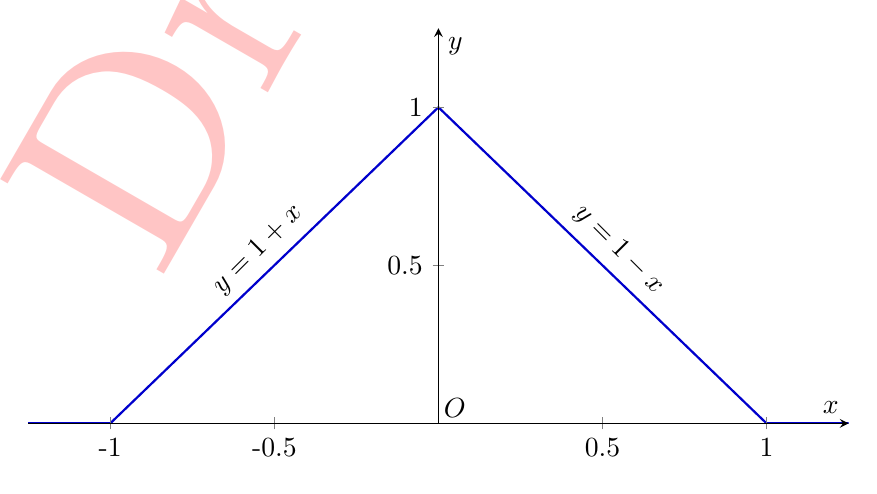
\begin{tikzpicture}
			\begin{axis}[
				axis lines=middle,
				xmin=-2.5, xmax=2.5,
				ymin=0, ymax=2.5,
				xtick={-2,-1,0,1,2},             
				xticklabels={-1,-0.5,0,0.5,1},       
				ytick={0,1,2},
				yticklabels={0,0.5,1},
				width=12cm, height=6.6cm,
				xlabel={$x$}, ylabel={$y$},
				enlargelimits=false,
				axis on top,                     
				]       % mũi tên trục
				
				\addplot[
				draw=blue!80!black,
				thick
				] coordinates {(-2,0) (0,2)};
				
				\addplot[
				draw=blue!80!black,
				thick
				] coordinates {(0,2) (2,0)};
				
				\addplot[
				draw=blue!80!black,
				thick
				] coordinates {(-2.5,0) (-2,0)};
				
				\addplot[
				draw=blue!80!black,
				thick
				] coordinates {(2,0) (2.5,0)};
				
				%--- Viết phương trình biên ---
				\node[rotate=45] at (axis cs:-1.1,1.1) {$y=1+x$};
				\node[rotate=-45] at (axis cs:1.1,1.1) {$y=1-x$};
				
				
				\node at (axis cs:0.1,0.1) {$O$};
				
			\end{axis}
		\end{tikzpicture}
	\end{center}
	
	\textit{Giải.} Áp dụng công thức tích phân từng phần, ta có biến đổi Fourier \begin{align*}
		\widehat\Lambda(s)&=\int_{-\infty}^\infty\Lambda(x)\mathrm e^{-2\pi\mathrm isx}\mathrm dx\\
		\noalign{\vskip5pt}
		&=\int_{-1}^0(1+x)\mathrm e^{-2\pi\mathrm isx}\mathrm dx+\int_0^1(1-x)\mathrm e^{-2\pi\mathrm isx}\mathrm dx\\
		\noalign{\vskip5pt}
		&=\frac{1+2\pi\mathrm is-\mathrm e^{2\pi\mathrm is}}{4\pi^2s^2}-\frac{2\pi\mathrm is-1+\mathrm e^{-2\pi\mathrm is}}{4\pi^2s^2}\\
		\noalign{\vskip5pt}
		&=\frac{2-\mathrm e^{-2\pi\mathrm is}-\mathrm e^{2\pi\mathrm is}}{4\pi^2s^2}=\frac{2-2\cos(2\pi s)}{4\pi^2s^2}\\
		\noalign{\vskip5pt}
		&=\frac{\sin^2(\pi s)}{\pi^2s^2}=\text{sinc}^2s.
	\end{align*}
	
	\textbf{Ví dụ 2:} \textit{Tìm biến đổi Fourier của hàm hình vuông sau} $$\Pi(t)=\begin{cases}
		\begin{array}{ll}
			1, & |t|<0.5,\\
			0, & |t|>0.5.
		\end{array}
	\end{cases}$$
	\begin{center}
		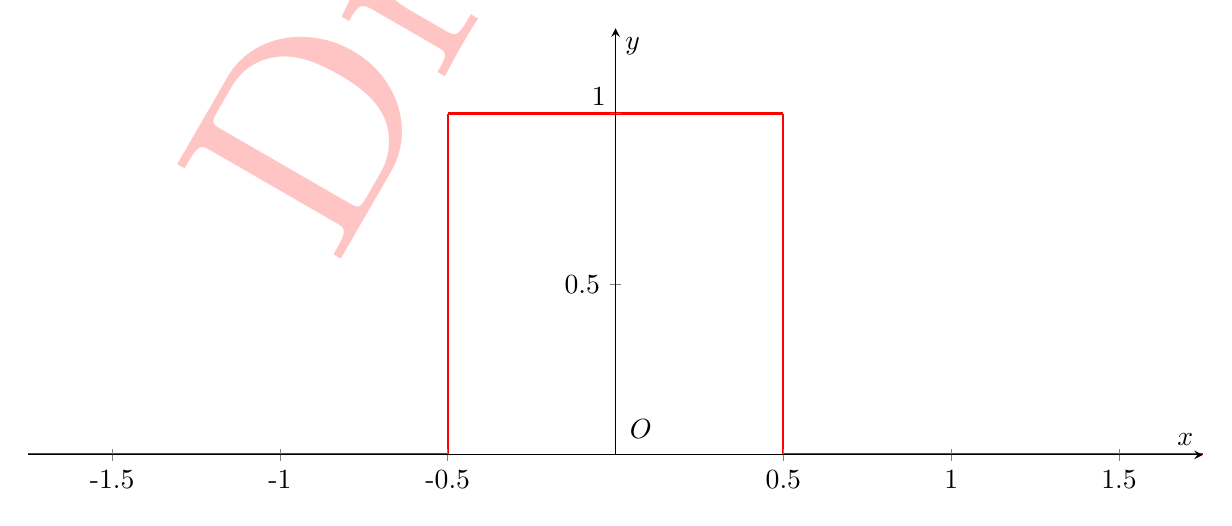
\begin{tikzpicture}
			\begin{axis}[
				axis lines=middle,
				xmin=-3.5, xmax=3.5,
				ymin=0, ymax=2.5,
				xtick={-3,-2,-1,0,1,2,3},             
				xticklabels={-1.5,-1,-0.5,0,0.5,1,1.5},       
				ytick={0,1,2},
				yticklabels={0,0.5},
				width=16.5cm, height=7cm,
				xlabel={$x$}, ylabel={$y$},
				enlargelimits=false,
				axis on top,                     
				]       % mũi tên trục
				
				\addplot[
				draw=red!100!black,
				very thick
				] coordinates {(-3.5,0) (-1,0)};
				
				\addplot[
				draw=red!100!black,
				thick
				] coordinates {(-1,0) (-1,2)};
				
				\addplot[
				draw=red!100!black,
				thick
				] coordinates {(-1,2) (1,2)};
				
				\addplot[
				draw=red!100!black,
				thick
				] coordinates {(1,2) (1,0)};
				
				\addplot[
				draw=red!100!black,
				very thick
				] coordinates {(1,0) (3.5,0)};
				
				\node at (axis cs:0.15,0.15) {$O$};
				\node at (axis cs:-0.1,2.1) {1};
				
			\end{axis}
		\end{tikzpicture}
	\end{center}
	
	\textit{Giải.} Ta tính $$\widehat\Pi(t)=\int_{-\infty}^\infty\Pi(t)\mathrm e^{-2\pi\mathrm ist}\mathrm dt=\int_{-0,5}^{0,5}\mathrm e^{-2\pi\mathrm ist}\mathrm dt=\frac{-\mathrm e^{-2\pi\mathrm ist}}{2\pi\mathrm is}\Bigg|_{-0,5}^{0,5}=\frac{\sin(\pi s)}{\pi s}=\operatorname{sinc}s.$$
	
	\textbf{Ví dụ 3:} \textit{Tìm biến đổi Fourier của hàm sau} $$f(t)=\begin{cases}
		\begin{array}{ll}
			0, & t\le0, \\
			\mathrm e^{-2t}, & t>0.
		\end{array}
	\end{cases}$$
	
	\textit{Giải.} Ta tính \begin{align*}
		\widehat f(s)&=\int_{-\infty}^\infty f(t)\mathrm e^{-2\pi\mathrm ist}\mathrm dt=\int_0^\infty\mathrm e^{-2t}\mathrm e^{-2\pi\mathrm ist}\mathrm dt\\
		\noalign{\vskip5pt}
		&=\int_0^\infty\mathrm e^{(-2\pi\mathrm is-2)t}\mathrm dt\\
		\noalign{\vskip5pt}
		&=\frac{\mathrm e^{(-2\pi\mathrm is-2)t}}{-2\pi\mathrm is-2}\Bigg|_{t\to\infty}-\frac{\mathrm e^{(-2\pi\mathrm is-2)t}}{-2\pi\mathrm is-2}\Bigg|_{t=0}\\
		\noalign{\vskip5pt}
		&=0+\frac{1}{2\pi\mathrm is+2}=\frac{1}{2\pi\mathrm is+2}.
	\end{align*}
	\subsection{Tính đối ngẫu của $\mathcal F$ và $\mathcal F^{-1}$. Tín hiệu ngược}
	\vspace{2mm}
	\quad\,\,Ta có các tính chất đối ngẫu sau: $\color{blue}\mathcal Ff(-s)=\mathcal F^{-1}f(s)$ và $\color{blue}\mathcal F^{-1}f(-s)=\mathcal Ff(s)$.\vskip7pt
	$\bullet~$\textbf{Tín hiệu lùi:} Với một hàm (hay "tín hiệu") $f$ thì \textbf{\color{red}tín hiệu lùi $f^-$} của $f$ được định nghĩa bởi $$\color{blue}f^-(t)=f(-t).$$
	\quad\,$\bullet~$Các kết quả cần nhớ:\begin{align*}
		&(\mathcal Ff)^-=\mathcal F^{-1}f=\mathcal Ff^-,\\
		&\left(\mathcal F^{-1}f\right)^-=\mathcal Ff=\mathcal F^{-1}f^-,\\
		&\mathcal F(\mathcal Ff)=f^-.
	\end{align*}
	\subsection{Bảng biến đổi Fourier của một số hàm}
	\begin{multicols}{2}
		\begin{center}
			\renewcommand{\arraystretch}{2.0}
			\begin{tabular}{|c|c|}
				\hline
				\textbf{\color{red}Hàm số} & \textbf{\color{red}Biến đổi Fourier} \\ \hline 
				$f(x-a)$ & $\widehat f(s)\mathrm e^{2\pi\text{i}sa}$ \\[4pt] \hline 
				$f(ax)$ & $\dfrac{1}{|a|}\widehat f\left(\dfrac sa\right)$ \\[4pt] \hline 
				$f(x)\mathrm e^{\text{i}ax}$ & $\widehat f\left(s-\dfrac{a}{2\pi}\right)$ \\[4pt] \hline
				$\overline{f(x)}$ & $\overline{\widehat f(-s)}$ \\[4pt] \hline
				$f(x)\cos(ax)$ & $\dfrac{\widehat f\left(s-\frac{a}{2\pi}\right)+\widehat f\left(s+\frac{a}{2\pi}\right)}{2}$ \\[4pt] \hline
				$f(x)\sin(ax)$ & $\dfrac{\widehat f\left(s-\frac{a}{2\pi}\right)-\widehat f\left(s+\frac{a}{2\pi}\right)}{2\text{i}}$ \\[4pt] \hline
			\end{tabular}
		\end{center}
		\columnbreak
		\begin{center}
			\renewcommand{\arraystretch}{2.0}
			\begin{tabular}{|c|c|}
				\hline
				\textbf{\color{red}Hàm số} & \textbf{\color{red}Biến đổi Fourier} \\ \hline 
				$\Pi(ax)$ & $\dfrac{1}{|a|}\text{sinc}\left(\dfrac sa\right)$ \\[4pt] \hline 
				$\text{sinc}(ax)$ & $\dfrac{1}{|a|}\Pi\left(\dfrac sa\right)$ \\[4pt] \hline 
				$\text{sinc}^2(ax)$ & $\dfrac{1}{|a|}\Lambda\left(\dfrac sa\right)$ \\[4pt] \hline
				$\Lambda(ax)$ & $\dfrac{1}{|a|}\text{sinc}^2\left(\dfrac sa\right)$ \\[4pt] \hline
				$\mathrm e^{-ax^2}$ & $\sqrt{\dfrac\pi a}\exp\left(-\dfrac{\pi^2s^2}{a}\right)$ \\[4pt] \hline
				$\mathrm e^{-a|x|}$ & $\dfrac{2a}{a^2+4\pi^2s^2}$ \\[4pt] \hline
			\end{tabular}
		\end{center}
	\end{multicols}
	\subsection{Tích chập}
	\vspace{2mm}
	\quad\,\,\,\textbf{\color{red}Tích chập (Convolution)} của hai hàm $g(t)$ và $f(t)$ được định nghĩa bởi $$\boxed{\color{blue}(g*f)(t):=\displaystyle\int_{-\infty}^\infty g(t-x)f(x)\text{d}x=\displaystyle\int_{-\infty}^\infty g(x)f(t-x)\text{d}x.}$$
	
	Tích chập có các tính chất: giao hoán, kết hợp, kết hợp với phép nhân vô hướng, và phân phối.\vskip7pt
	$\bullet~$\textbf{Mối liên hệ giữa biến đổi Fourier và tích chập:} Tích chập trong miền thời gian tương ứng với phép nhân trong miền tần số, và ngược lại. Nói cách khác\begin{align*}
		&\mathcal F(g*f)=\mathcal Fg\cdot\mathcal Ff,\\
		&\mathcal F^{-1}(g*f)=\mathcal F^{-1}g\cdot\mathcal F^{-1}f,\\
		&\mathcal F(gf)=\mathcal Fg*\mathcal Ff.
	\end{align*}
	\subsection{Biến đổi Fourier của đạo hàm cấp cao - Ứng dụng giải ODE và PDE}
	\vspace{2mm}
	\quad\,\,\,Giả sử $f(t)\rightarrow0$ khi $|t|\rightarrow\infty$. Khi đó, biến đổi Fourier của đạo hàm cấp $n$ là $$\boxed{\color{blue}\left(\mathcal Ff^{(n)}\right)(s)=(-2\pi\text{i}s)^n\mathcal Ff(s).}$$
	
	\textbf{Ví dụ 1:} \textit{Giải phương trình vi phân sau bằng phép biến đổi Fourier.} $$\frac{\mathrm d^2}{\mathrm dt^2}u(t)-2u(t)=-f(t).$$
	
	\textit{Giải.} Áp dụng biến đổi Fourier cho hai vế của phương trình, ta được \begin{align*}
		&\mathcal F\left[\frac{\mathrm d^2}{\mathrm dt^2}u(t)-2u(t)\right](s)=\mathcal F[-f(t)](s)\\
		\Leftrightarrow~&\mathcal F(u'')(s)-2\mathcal Fu(s)=-\mathcal Ff(s)\\
		\Leftrightarrow~&(-2\pi\mathrm is)^2\mathcal Fu(s)-2\mathcal Fu(s)=-\mathcal Ff(s)\\
		\Leftrightarrow~&-4\pi^2s^2\mathcal Fu(s)-2\mathcal Fu(s)=-\mathcal Ff(s).
	\end{align*}
	
	Như vậy, ta tìm được $$\mathcal Fu(s)=\frac{1}{4\pi^2s^2+2}\mathcal Ff(s).$$
	
	Đặt $\widehat g(s)=\mathcal Fg(s)=\dfrac{1}{4\pi^2s^2+2}$, nên ta có $$\mathcal Fu(s)=\mathcal Fg(s)\mathcal Ff(s)\iff u(t)=(g*f)(t).$$
	
	Ta cần xác định hàm $g$. Tra bảng ở mục 8.4, ta có $$\mathcal F\big(\mathrm e^{-|a|t}\big)(s)=\frac{2a}{a^2+4\pi^2s^2}.$$
	
	Ta cho $a=\sqrt2$. Khi này $\mathcal F\big(\mathrm e^{-\sqrt2t}\big)(s)=\dfrac{2\sqrt2}{2+4\pi^2s^2}$, tức là $g(t)=\dfrac{1}{2\sqrt2}\mathrm e^{-\sqrt2t}$. Vì vậy ta tìm được $$u(t)=(g*f)(t)=\frac{\sqrt2}{4}\int_{-\infty}^\infty\mathrm e^{-\sqrt2|t-x|}f(x)\mathrm dx,$$
	là nghiệm của phương trình vi phân đã cho.\\
	
	\textbf{Ví dụ 2:} \textit{Tìm nghiệm $u(x,t)$ của phương trình truyền nhiệt trên một thanh kim loại dài vô hạn} $$\frac{\partial u}{\partial t}=\frac14\frac{\partial^2u}{\partial x^2},~~-\infty<x<\infty,~t>0,$$
	\textit{với điều kiện đầu} $u(x,0)=f(x)$.\\
	
	\textit{Giải.} Vì $x\in\mathbb R$ nên ta áp dụng biến đổi Fourier theo biến $x$ ở hai vế của phương trình để có \begin{align*}
		&\mathcal F[u_t(x,t)](s,t)=\frac14(-2\pi\mathrm is)^2\mathcal Fu(s,t)\\
		\noalign{\vskip3pt}
		\Leftrightarrow~&\mathcal F[u_t(x,t)](s,t)=-\pi^2s^2\mathcal Fu(s,t)\\
		\Rightarrow~&\frac{\partial}{\partial t}\mathcal Fu(s,t)=-\pi^2s^2\mathcal Fu(s,t)\\
		\noalign{\vskip3pt}
		\Rightarrow~&\mathcal Fu(s,t)=\mathcal Fu(s,0)\mathrm e^{-\pi^2s^2t}.
	\end{align*}
	
	Ta có $$\mathcal Fu(s,0)=\int_{-\infty}^\infty u(x,0)\mathrm e^{-2\pi\mathrm isx}\mathrm dx=\int_{-\infty}^\infty f(x)\mathrm e^{-2\pi\mathrm isx}\mathrm dx=\mathcal Ff(s),$$
	vì vậy ta viết lại thành $$\mathcal Fu(s,t)=\mathcal Ff(s)\mathrm e^{-\pi^2s^2t}.$$
	
	Gọi $g(x,t)$ là hàm thỏa mãn $\mathcal Fg(s,t)=\mathrm e^{-\pi^2s^2t}$. Như vậy $$\mathcal Fu(s,t)=\mathcal Ff(s)\cdot\mathcal Fg(s,t).$$
	
	Mặt khác, từ công thức $$\mathcal F\left[\frac{1}{\sigma\sqrt{2\pi}}\exp\left(-\frac{x^2}{2\sigma^2}\right)\right](s)=\mathrm e^{-2\pi^2\sigma^2s^2},$$
	với $\sigma^2=\dfrac t2$, ta tìm được $$g(x,t)=\frac{1}{\sqrt{\pi t}}\mathrm e^{-x^2/t},~~\forall t\ge0.$$
	
	Do đó nghiệm của phương trình đã cho là \begin{align*}
		u(x,t)&=g(x,t)*f(x)=\left(\frac{1}{\sqrt{\pi t}}\mathrm e^{-x^2/t}\right)*f(x)\\
		\noalign{\vskip7pt}
		&=\frac{1}{\sqrt{\pi t}}\int_{-\infty}^\infty\exp\left[-\frac{(x-y)^2}{t}\right]f(y)\mathrm dy.
	\end{align*}
	
	Vai trò của tích chập trong ví dụ này là "chia đều" nhiệt độ ban đầu cho mọi điểm trong vật khi $t>0$.\\
	
	\textbf{Ví dụ 3:} \textit{Tìm nghiệm $u(x,t)$ của phương trình truyền sóng trên một sợi dây dài vô hạn} $$\frac{\partial^2u}{\partial t^2}=4\frac{\partial^2u}{\partial x^2},~~-\infty<x<\infty,~t>0,$$
	\textit{với điều kiện đầu $u(x,0)=f(x)$ và $u_t(x,0)=g(x)$. Khi sử dụng biến đổi Fourier, một trong những giả thiết từ vật lý là $|u(x,t)|\to0~\text{khi}~|t|\to\infty.$}\\
	
	\textit{Giải.} Vì $x\in\mathbb R$ nên ta áp dụng biến đổi Fourier theo biến $x$ ở hai vế của phương trình để có \begin{align*}
		&\mathcal F[u_{tt}(x,t)](s,t)=4(-2\pi\mathrm is)^2\mathcal Fu(s,t)\\
		\Rightarrow~&\frac{\partial^2}{\partial t^2}\mathcal Fu(s,t)+16\pi^2s^2\mathcal Fu(s,t)=0.
	\end{align*}
	
	Khi $s=0$ thì $\mathcal Fu(s,t)=A+Bt$ và $|\mathcal Fu(s,t)|\to\infty$ khi $|t|\to\infty$, trái với giả thiết. Vậy ta loại $s\ne0$.\\
	
	Giải bài toán trong miền tần số rồi lấy biến đổi Fourier ngược, ta có $$\mathcal Fu(s,t)=\widehat A(s)\cos(4\pi st)+\widehat B(s)\sin(4\pi st).$$
	
	Điều kiện đầu $u(x,0)=f(x)$ cho ta $$\mathcal Fu(s,0)=\widehat A(s)=\int_{-\infty}^\infty u(x,0)\mathrm e^{-2\pi\mathrm isx}\mathrm dx=\int_{-\infty}^\infty f(x)\mathrm e^{-2\pi\mathrm isx}\mathrm dx=\mathcal Ff(s).$$
	
	Tiếp theo, ta lấy đạo hàm theo $t$ cho biến đổi Fourier $$\mathcal Fu_t(s,t)=-4\pi s\widehat A(s)\sin(4\pi st)+4\pi s\widehat B(s)\cos(4\pi st),$$
	nên với $t=0$, ta sử dụng điều kiện đầu $u_t(x,0)=g(x)$ như sau $$\mathcal Fu_t(s,0)=4\pi s\widehat B(s)=\int_{-\infty}^\infty u_t(x,0)\mathrm e^{-2\pi\mathrm isx}\mathrm dx=\int_{-\infty}^\infty g(x)\mathrm e^{-2\pi\mathrm isx}\mathrm dx=\mathcal Fg(s),$$
	vì vậy ta thu được $\widehat B(s)=\dfrac{1}{4\pi s}\mathcal Fg(s)$. Thay vào $\mathcal Fu(s,t)$ vừa tìm được, ta có $$\mathcal Fu(s,t)=\mathcal Ff(s)\cos(4\pi st)+\frac{\mathcal Fg(s)}{4\pi s}\sin(4\pi st).$$
	
	Vì $\mathcal Ff(s)\cos(4\pi st)=\dfrac{\mathcal Ff(s)}{2}\big(\mathrm e^{4\pi\mathrm ist}+\mathrm e^{-4\pi\mathrm ist}\big)$ nên ta có $$\mathcal F^{-1}[\mathcal Ff(s)\cos(4\pi st)]=\frac12f(x-2t)+\frac12f(x+2t).$$
	
	Đặt $G(x)=\displaystyle\int_0^xg(\xi)\mathrm d\xi$, tức là $G'=g$. Lấy biến đổi Fourier hai vế, ta được $$\mathcal Fg(s)=\mathcal F[G'(x)](s)=2\pi\mathrm is\mathcal FG(s)\iff\frac{\mathcal Fg(s)}{2\pi s}=\mathrm i\mathcal FG(s).$$
	
	Ta tính \begin{align*}
		\mathcal F^{-1}\left[\frac{\mathcal Fg(s)}{4\pi s}\sin(4\pi st)\right]&=\mathcal F^{-1}\left[\frac{\mathrm i}{2}\mathcal FG(s)\frac{\mathrm e^{-4\pi\mathrm ist}-\mathrm e^{4\pi\mathrm ist}}{2\mathrm i}\right]\\
		\noalign{\vskip5pt}
		&=\frac14G(x+2t)-\frac14G(x-2t)\\
		\noalign{\vskip5pt}
		&=\frac14\int_0^{x+2t}g(\xi)\mathrm d\xi-\frac14\int_0^{x-2t}g(\xi)\mathrm d\xi\\
		\noalign{\vskip5pt}
		&=\frac14\int_{x-2t}^{x+2t}g(\xi)\mathrm d\xi.
	\end{align*}
	
	Lấy biến đổi Fourier ngược, ta được nghiệm của phương trình truyền sóng là \begin{align*}
		u(x,t)=\mathcal F^{-1}[\mathcal Fu(s,t)]&=\mathcal F^{-1}[\mathcal Ff(s)\cos(4\pi st)]+\mathcal F^{-1}\left[\frac{\mathcal Fg(s)}{4\pi s}\sin(4\pi st)\right]\\
		\noalign{\vskip5pt}
		&=\frac12f(x-2t)+\frac12f(x+2t)+\frac14\int_{x-2t}^{x+2t}g(\xi)\mathrm d\xi.
	\end{align*}
	\subsection{Bài tập tự luyện}
	\textbf{\color{red}\underline{Bài 1:}} Tìm biến đổi Fourier của các hàm sau.\begin{multicols}{2}
		\begin{flushleft}
			\textbf{a) }$f(x)=\begin{cases}
				\begin{array}{ll}
					4, & -\alpha\le x\le\alpha, \\
					0, & |x|>\alpha;
				\end{array}
			\end{cases}$\\\vspace{3mm}
			\textbf{c) }$f(x)=\mathrm e^{-2|x|}\cos(3x);$
		\end{flushleft}
		\columnbreak
		\begin{flushleft}
			\textbf{b) }$f(x)=\begin{cases}
				\begin{array}{ll}
					\sin x, & -3\le x\le3, \\
					0, & |x|>3;
				\end{array}
			\end{cases}$\\\vspace{3mm}
			\textbf{d) }$f(x)=\mathrm e^{-4x^2}$.
		\end{flushleft}
	\end{multicols}
	\begin{flushleft}
		\textbf{\color{red}\underline{Bài 2:}} Chứng minh phép biến đổi sau 
	\end{flushleft}
	$$\mathcal F[x^nf(x)](s)=\left(\dfrac{\text{i}}{2\pi}\right)^n\dfrac{\text{d}^n}{\text{d}s^n}\mathcal Ff(s).$$
	\textbf{\color{red}\underline{Bài 3:}} Áp dụng Bài 2 để tìm các biến đổi Fourier sau. \begin{multicols}{2}
		\begin{flushleft}
			\textbf{a) }$\mathcal F\left(x^2\mathrm e^{-25x^2}\right)$;
		\end{flushleft}
		\columnbreak
		\begin{flushleft}
			\textbf{b) }$\mathcal F\left(\dfrac{\sin(5x)}{x^2+36}\right)$.
		\end{flushleft}
	\end{multicols}
	\begin{flushleft}
		\textbf{\color{red}\underline{Bài 4:}} Bằng phương pháp biến đổi Fourier, hãy tìm nghiệm $u(x,t)$ của các PDE sau.
	\end{flushleft}
	\begin{multicols}{2}
		\begin{flushleft}
			\textbf{a) }$\begin{cases}
			\begin{array}{ll}
				u_t=u_{xx}, & -\infty<x<\infty,~t>0,\\
				u(x,0)=\mathrm e^{-2|x|}, & -\infty<x<\infty;
			\end{array}
			\end{cases}$\\\vspace{18mm}
			\textbf{c) }$\begin{cases}
				\begin{array}{ll}
					u_{tt}=u_{xxxx}, & -\infty<x<\infty,~t>0,\\
					u(x,0)=x\mathrm e^{-x^2}, & -\infty<x<\infty,\\
					u_t(x,0)=\mathrm e^{-x^2}, & -\infty<x<\infty;
				\end{array}
			\end{cases}$
		\end{flushleft}
		\columnbreak
		\begin{flushleft}
			\textbf{b) }$\begin{cases}
			\begin{array}{ll}
				u_{tt}=u_{xx}, & -\infty<x<\infty,~t>0,\\
				\noalign{\vskip6pt}
				u(x,0)=\mathrm e^{-x^2}, & -\infty<x<\infty,\\
				\noalign{\vskip4pt}
				u_t(x,0)=\dfrac{2x}{1+x^4}, & -\infty<x<\infty;
				\end{array}
			\end{cases}$\\\vspace{9mm}
			\textbf{d) }$\begin{cases}
				\begin{array}{ll}
					u_{t}+tu_{x}=t\mathrm e^{-|x|}, & -\infty<x<\infty,~t>0,\\
					\noalign{\vskip7pt}
					u(x,0)=\dfrac{1}{1+x^2}, & -\infty<x<\infty.
				\end{array}
			\end{cases}$
		\end{flushleft}
	\end{multicols}
	\newpage
	\section{Truyền nhiệt trên thanh kim loại dài vô hạn}
	\subsection{Phương trình parabolic}
	\vspace{2mm}
	\quad\,\,\,\textbf{\color{red}Phương trình parabolic cấp hai} xảy ra trong quá trình truyền dẫn và khuếch tán nhiệt. Bây giờ ta sẽ gọi $u(x,t)$ là nhiệt độ trong môi trường tại điểm $M(x)\in\mathbb R^n$ tại thời điểm $t$.\\
	
	Xét một \textbf{môi trường đẳng hướng} - tức là cùng cấu trúc và tính chất theo mọi hướng, ta gọi:\vskip10pt
	\quad$\bullet~\rho(M)$ là mật độ của môi trường;\vskip7pt
	\quad$\bullet~c(M)$ là nhiệt dung riêng;\vskip7pt
	\quad$\bullet~k(M)$ là độ dẫn nhiệt tại điểm $M$: Bên trong vật thể, nhiệt độ có thể được sinh ra hay hấp thu (chẳng hạn, nhờ phản ứng hóa học).\\
	
	Gọi $F(M,t)$ là mật độ của nguồn nhiệt tại điểm $M$ ở thời điểm $t$. Theo Định luật Fourier, bỏ qua quán tính của chuyển động phân tử, ta có phương trình $$c\rho\frac{\partial u}{\partial t}=\nabla\cdot(k\nabla u)+F(M,t).$$
	
	Khi môi trường là thuần nhất, tức $c$, $\rho$ và $k$ là các hằng số, ta có phương trình \begin{equation} \tag{9.1} \label{9.1}
		\frac{\partial u}{\partial t}=a^2\Delta u+f,
	\end{equation}
	trong đó $a^2=\dfrac{k}{c\rho},\,f=\dfrac{F}{c\rho}$ và $\Delta u$ là toán tử Laplace của $u$. Phương trình \ref{9.1} được gọi là \textbf{\color{red}phương trình nhiệt}.\\
	
	Ta sẽ giới hạn khảo sát phương trình nhiệt với một biến không gian $(x\in\mathbb R)$, nghĩa là sự truyền nhiệt trong một thanh đồng chất. Bài toán trở thành tìm nghiệm $u:\mathbb R\times(0,\infty)\to\mathbb R$ của phương
	trình \begin{equation} \tag{9.2} \label{9.2}
		\frac{\partial u}{\partial t}=a^2\frac{\partial^2u}{\partial x^2}+f(x,t).
	\end{equation}
	
	Ở đây $f(x,t)$ được gọi là nguồn nhiệt bên ngoài, và $u(x,t)$ là nhiệt độ tại vị trí $x$ ở thời điểm $t>0$. Hằng số $a$ được gọi là \textbf{hệ số dẫn nhiệt} (hay hệ số truyền nhiệt, thermal
	diffusivity), và có đơn vị là m$^2$/s.
	\subsection{Nghiệm tổng quát}
	\vspace{2mm}
	\quad\,\,\,Ta xét phương trình nhiệt \ref{9.2} ở dạng thuần nhất, tức $f(x,t)\equiv0$, nghĩa là trường hợp không có nguồn nhiệt bên ngoài tác động lên thanh đồng chất.
	\vspace{2mm}
	\begin{tcolorbox}[enhanced,colback=blue!5!white,colframe=blue!75!black,sharp corners=all,shadow={0mm}{0mm}{-1.5mm}%
		{fill=blue!75!red,opacity=0.3},title=\textbf{Dạng của bài toán}]
		$$\begin{cases}
			\begin{array}{ll}
				u_t=a^2u_{xx}, & -\infty<x<\infty,~t>0,\\
				u(x,0)=\varphi(x), & -\infty<x<\infty,
			\end{array}
		\end{cases}$$
		với $\varphi(x)$ là nhiệt độ của thanh kim loại tại thời điểm đầu, và $a$ là hệ số dẫn nhiệt. Các đầu thanh kim loại được cách nhiệt.
	\end{tcolorbox}
	\vspace{2mm}
	Áp dụng công thức tích phân Poisson, ta có nghiệm của bài toán là $$u(x,t)=\dfrac{1}{2a\sqrt{\pi t}}\varphi(x)*\exp\left(-\frac{x^2}{4a^2t}\right)=\dfrac{1}{2a\sqrt{\pi t}}\displaystyle\int_{-\infty}^\infty\varphi(y)\exp\left[-\frac{(x-y)^2}{4a^2t}\right]\text{d}y.$$
	
	\textbf{Ví dụ:} \textit{Tìm nghiệm của bài toán truyền nhiệt sau} $$\begin{cases}
		\begin{array}{ll}
			u_t=4u_{xx}, & -\infty<x<\infty,~t>0,\\
			u(x,0)=\mathrm e^{-x^2/2}, & -\infty<x<\infty.
		\end{array}
	\end{cases}$$
	
	Áp dụng công thức tích phân Poisson, ta có \begin{align*}
		u(x,t)&=\frac{1}{4\sqrt{\pi t}}\int_{-\infty}^\infty\mathrm e^{-y^2/2}\exp\left[-\frac{(x-y)^2}{16t}\right]\mathrm dy\\
		\noalign{\vskip5pt}
		&=\frac{1}{4\sqrt{\pi t}}\int_{-\infty}^\infty\exp\left(-\frac{y^2}{2}-\frac{x^2}{16t}+\frac{xy}{8t}-\frac{y^2}{16t}\right)\mathrm dy\\
		\noalign{\vskip5pt}
		&=\frac{1}{4\sqrt{\pi t}}\int_{-\infty}^\infty\exp\left(-\frac{y^2}{2}-\frac{y^2}{16t}+\frac{2xy}{16t}-\frac{x^2}{16t}\right)\mathrm dy\\
		\noalign{\vskip5pt}
		&=\frac{1}{4\sqrt{\pi t}}\int_{-\infty}^\infty\exp\left[-\frac{8t+1}{16t}y^2+2\sqrt{\frac{8t+1}{16t}}y\sqrt{\frac{16t}{8t+1}}\frac{x}{16t}-\frac{x^2}{16t(8t+1)}+\frac{x^2}{16t(8t+1)}-\frac{x^2}{16t}\right]\mathrm dy\\
		\noalign{\vskip4pt}
		&=\frac{1}{4\sqrt{\pi t}}\int_{-\infty}^\infty\exp\left[-\left(\sqrt{\frac{8t+1}{16t}}y-\frac{1}{\sqrt{16t(8t+1)}}x\right)^2+\frac{x^2}{16t+2}\right]\mathrm dy.
	\end{align*}
	
	Đặt $z=\sqrt{\dfrac{8t+1}{16t}}y-\dfrac{1}{\sqrt{16t(8t+1)}}x$, khi này biểu thức trở thành \begin{align*}
		u(x,t)&=\frac{1}{4\sqrt{\pi t}}\sqrt{\frac{16t}{8t+1}}\exp\left(\frac{x^2}{16t+2}\right)\int_{-\infty}^\infty\mathrm e^{-z^2}\mathrm dz\\
		\noalign{\vskip5pt}
		&=\frac{1}{\sqrt{\pi}}\frac{1}{\sqrt{8t+1}}\exp\left(\frac{x^2}{16t+2}\right)\sqrt\pi\\
		\noalign{\vskip5pt}
		&=\frac{1}{\sqrt{8t+1}}\exp\left(\frac{x^2}{16t+2}\right).
	\end{align*}
	
	Vậy nghiệm của bài toán là $u(x,t)=\dfrac{1}{\sqrt{8t+1}}\exp\left(\dfrac{x^2}{16t+2}\right).$
	\subsection{Nghiệm cơ bản với hàm Dirac--delta}
	\vspace{2mm}
	$\bullet~$\textbf{\color{red}Hàm Dirac--$\delta$:} Là hàm được định nghĩa một cách hình thức như sau
	\vskip7pt
	i) $\delta(x-x_0)=\begin{cases}
		\begin{array}{ll}
			0, & x\ne x_0, \\
			+\infty, & x=x_0;
		\end{array}
	\end{cases}$
	\vskip7pt
	ii) $\displaystyle\int_{-\infty}^\infty\delta(x-x_0)\text{d}x=1$, hoặc $\displaystyle\int_\alpha^\beta\delta(x-x_0)\text{d}x=1$ với mọi khoảng $(\alpha,\beta)$ chứa điểm $x=x_0$;
	\vskip7pt
	iii) $\displaystyle\int_\alpha^\beta f(x)\delta(x-x_0)\text{d}x=\begin{cases}
		\begin{array}{ll}
			f(x_0), & x_0\in(\alpha,\beta),\\
			0, & x_0\notin(\alpha,\beta).
		\end{array}
	\end{cases}$\\\\
	$\bullet~$Ta có \textbf{\color{red}nghiệm cơ bản} của phương trình truyền nhiệt là $$G(x,t,\lambda)=\dfrac{1}{2a\sqrt{\pi t}}\exp\left[-\frac{(x-y)^2}{4a^2t}\right].$$
	Khi $\lambda=0$ thì lúc đó $G(x,t,0)$ là nghiệm của bài toán $$\begin{cases}
		\begin{array}{ll}
			u_t=a^2u_{xx}, & -\infty<x<\infty,~t>0,\\
			u(x,0)=\delta(x), & -\infty<x<\infty.
		\end{array}
	\end{cases}$$
	\subsection{Bài tập tự luyện}
	Tìm nghiệm của các bài toán khuếch tán sau.\\\\
	\textbf{a) }$\begin{cases}
		\begin{array}{ll}
			u_t-9u_{xx}=0, & -\infty<x<\infty,~t>0,\\
			u(x,0)=\sqrt{2\pi}\mathrm e^{-5x^2}, & -\infty<x<\infty;
		\end{array}
	\end{cases}$\\\\\\
	\textbf{b) }$\begin{cases}
		\begin{array}{ll}
			u_t-25u_{xx}=0, & -\infty<x<\infty,~t>0,\\
			u(x,0)=f(x), & -\infty<x<\infty,
		\end{array}
	\end{cases}$ với $f(x)=\begin{cases}
		\begin{array}{ll}
			\sin x, & |x|\le\pi,\\
			0, & |x|>\pi;
		\end{array}
	\end{cases}$\\\\\\
	\textbf{c) }$\begin{cases}
		\begin{array}{ll}
			u_t-16u_{xx}=0, & -\infty<x<\infty,~t>0,\\
			u(x,0)=5\mathrm e^{-x^2/2}, & -\infty<x<\infty;
		\end{array}
	\end{cases}$\\\\\\
	\textbf{d) }$\begin{cases}
	\begin{array}{ll}
		u_t-4u_{xx}=0, & -\infty<x<\infty,~t>0,\\
		u(x,0)=\begin{cases}
		\begin{array}{ll}
			3, & x\ge0,\\
			0, & x<0,
		\end{array}
		\end{cases}, & -\infty<x<\infty.
	\end{array}
	\end{cases}$\\\\\\
	Gợi ý câu d: Sử dụng hàm lỗi (error function) erf$(x)=\dfrac{2}{\sqrt\pi}\displaystyle\int_0^x\mathrm e^{-z^2}\mathrm dz$ và đẳng thức $\displaystyle\int_{-\infty}^{\infty}\mathrm e^{-z^2}\mathrm dz=\sqrt\pi$.
	\newpage
	\section{Truyền nhiệt trên thanh kim loại dài hữu hạn}
	\subsection{Nguyên lý cực đại, cực tiểu của phương trình nhiệt}
	\vspace{2mm}
	\quad\,\,\,Cho phương trình nhiệt có nguồn nhiệt sau $$\dfrac{\partial u}{\partial t}-a^2\dfrac{\partial^2u}{\partial x^2}=F(x,t),~~(x,t)\in D=\{(x,t):0\le x\le L,~0\le t\le T\}.$$
	
	Giả sử $u(x,t)$ là nghiệm của phương trình, và liên tục trên $D$. Khi đó, tại ba thời điểm $x=0,\,x=L$ và $t=0$:
	\vskip7pt
	$\bullet~$Nếu $F>0$ thì $u(x,t)$ \textbf{\color{red}chỉ đạt giá trị nhỏ nhất;}
	\vskip7pt
	$\bullet~$Nếu $F<0$ thì $u(x,t)$ \textbf{\color{red}chỉ đạt giá trị lớn nhất;}
	\vskip7pt
	$\bullet~$Nếu $F=0$ thì $u(x,t)$ \textbf{\color{red}đạt giá trị lớn nhất và nhỏ nhất.}
	\subsection{Nguyên lý so sánh trong phương trình nhiệt}
	\vspace{2mm}
	\quad\,\,\,$\bullet~$\textbf{Loại I (Hệ quả của Nguyên lý cực đại):} \textit{Cho $u$ và $v$ là hai nghiệm của phương trình nhiệt trong miền $[0,L]\times[0,T]$. Nếu $u\le v$ trên biên $x=0,\,x=L$ và tại thời điểm $t=0$, thì $u\le v$ với mọi $(x,t)\in[0,L]\times[0,T]$.}
	\vskip7pt
	$\bullet~$\textbf{Loại II:} \textit{Cho $D=[0,L]\times[0,\infty)$ và $u,v$ là hai hàm trơn thỏa} $$\begin{cases}
		u_t-a^2u_{xx}=f(x,t),\\
		v_t-a^2v_{xx}=g(x,t),
	\end{cases}$$
	\textit{với mọi $(x,t)\in D$.}
	\begin{flushleft}
		\textit{Giả sử $f\le g$ trên $D$ và $u\le v$ trên biên $x=0,\,x=L$ và tại thời điểm $t=0$. Khi đó $u\le v$ trên $D$.}
	\end{flushleft}
	
	\textbf{Ví dụ:} \textit{Cho phương trình nhiệt} $$\begin{cases}
	\begin{array}{ll}
		u_t-2u_{xx}=0, & 0<x<2,\,t>0,\\
		u(0,t)=u(2,t)=0, & t\ge0,\\
		u(x,0)=x(2-x), & 0<x<2.
	\end{array}
	\end{cases}$$
	\textit{\color{violet}{a) Tìm giá trị lớn nhất của $u(x,t)$ trên miền $[0,2]\times[0,\infty)$.}}\vskip8pt
	Vì $u(0,t)=u(2,t)=0$ nên theo nguyên lý cực đại, $u$ đạt giá trị lớn nhất tại thời điểm $t=0$. Khi đó ta cần tìm giá trị lớn nhất của hàm $u(x,0)=x(2-x).$\vskip8pt
	Đây là hàm bậc hai với bề lõm quay xuống, nên dễ dàng tính được $\max u(x,0)=1$ khi $x=1$.\vskip8pt
	Do đó, giá trị lớn nhất của $u$ bằng 1 tại $(x,t)=(1,0)$.\\\\
	\textit{\color{violet}{b) Chứng tỏ rằng $0\le u(x,t)\le x(2-x)\mathrm e^{-4t}$ với mọi $(x,t)\in[0,2]\times[0,\infty)$.}}\vskip8pt
	Vì $u(0,t)=u(2,t)=0$ và $u(x,0)=x(2-x)\ge0$ với mọi $0\le x\le2$, nên nguyên lý cực đại cho ta $u\ge0$ với mọi $(x,t)\in[0,2]\times[0,\infty)$.\vskip8pt
	Đặt $v(x,t)=x(2-x)\mathrm e^{-4t}$. Ta tính $$\begin{cases}
			v_t-2v_{xx}=-4x(2-x)\mathrm e^{-4t}+4\mathrm e^{-4t}=\big(4x^2-8x+4\big)\mathrm e^{-4t},\\
			v(0,t)=v(2,t)=0,\\
			v(x,0)=x(2-x).
	\end{cases}$$
	
	Với $(x,t)\in[0,2]\times[0,\infty)$, ta có $$v_t-2v_{xx}=\big(4x^2-8x+4\big)\mathrm e^{-4t}\ge0,$$
	với dấu "=" xảy ra tại $x=1$. Áp dụng nguyên lý so sánh trong phương trình nhiệt (loại 2), ta suy ra được $$0\le u(x,t)\le v(x,t)=x(2-x)\mathrm e^{-4t}.$$
	\textit{\color{violet}{c) Cố định $x\in[0,2]$, hãy cho biết khi $t\to\infty$ thì $u(x,t)$ càng tiến về bao nhiêu?}}\vskip8pt
	Từ bất đẳng thức $$0\le u(x,t)\le x(2-x)\mathrm e^{-4t},~~0\le x\le2,~t\ge0$$
	ở câu b), ta cố định $x$ và cho $t\to\infty$. Vì $$\lim_{t\to\infty}\mathrm e^{-4t}=0,$$
	nên ta có $u(x,t)\to0$.
	\subsection{Phương trình truyền nhiệt không có nguồn nhiệt với điều kiện biên Dirichlet thuần nhất}
	\vspace{2mm}
	\begin{tcolorbox}[enhanced,colback=blue!5!white,colframe=blue!75!black,sharp corners=all,shadow={0mm}{0mm}{-1.5mm}%
		{fill=blue!75!red,opacity=0.3},title=\textbf{Dạng của bài toán}]
		$$\begin{cases}
			\begin{array}{ll}
				u_t=a^2u_{xx}, & 0<x<L,~t>0,\\
				u(0,t)=u(L,t)=0, & t\ge0,\\
				u(x,0)=\varphi(x), & 0\le x\le L,
			\end{array}
		\end{cases}$$
		với $\varphi(x)$ là nhiệt độ của thanh kim loại tại thời điểm đầu, và $a$ là hệ số dẫn nhiệt.\vskip7pt
		Hơn nữa, $u(0,t)=u(L,t)=0$ được gọi là \textit{điều kiện biên Dirichlet thuần nhất}.
	\end{tcolorbox}
	\vspace{2mm}
	Ta có nghiệm của bài toán là $$u(x,t)=\displaystyle\sum_{k=1}^\infty A_k\exp\left(-\frac{k^2\pi^2a^2t}{L^2}\right)\sin\dfrac{k\pi x}{L},$$
	với hệ số $A_k=\dfrac2L\displaystyle\int_0^L\varphi(x)\sin\dfrac{k\pi x}{L}\text{d}x.$\\
	
	\textbf{Ví dụ:} \textit{Giải bài toán truyền nhiệt sau} $$\begin{cases}
		\begin{array}{ll}
			u_t=u_{xx}, & 0<x<1,~t>0,\\
			u(0,t)=u(1,t)=0, & t\ge0,\\
			u(x,0)=x^2, & 0\le x\le 1.
		\end{array}
	\end{cases}$$
	
	\textit{Giải.} Bằng phương pháp tách biến Fourier, giả sử nghiệm của bài toán có dạng $$u(x,t)=X(x)T(t).$$
	
	Thay vào PDE ban đầu, ta có $$X(x)T'(t)=X''(x)T(t)\iff\frac{X''(x)}{X(x)}=\frac{T'(t)}{T(t)}=-\lambda,$$
	với $\lambda$ là hằng số tách biến. Khi đó ta được hai ODE sau $$\begin{cases}
		X''(x)+\lambda X(x)=0,\\
		T'(t)+\lambda T(t)=0.
	\end{cases}$$
	
	$\bullet~$Xét ODE $X''(x)+\lambda X(x)=0$. Điều kiện biên $u(0,t)=u(1,t)=0$ cho ta $X(0)=X(1)=0$. Trường hợp $\lambda<0$ và $\lambda=0$ cho ra nghiệm tầm thường $u(x,t)\equiv0$ (đọc lại slide bài giảng). Với $\lambda>0$, nghiệm của ODE đang xét là $$X(x)=C_1\cos\big(\sqrt\lambda x\big)+C_2\sin\big(\sqrt\lambda x\big).$$
	
	Điều kiện $X(0)=X(1)=0$ cho ta $$\begin{cases}
		C_1\cos0+C_2\sin0=0,\\
		C_1\cos\sqrt\lambda+C_2\sin\sqrt\lambda=0.
	\end{cases}$$
	
	Hệ luôn cho kết quả $C_1=0$. Vì ta cần tìm nghiệm không tầm thường nên định thức phải bằng 0, hay $$\begin{vmatrix}
		1&0\\
		\cos\sqrt\lambda&\sin\sqrt\lambda
	\end{vmatrix}=0\iff\sin\sqrt\lambda=0\iff\sqrt\lambda=k\pi,~~k=1,2,\ldots,$$
	do đó ta có các trị riêng $\lambda=\lambda_k=k^2\pi^2,\,k\in\mathbb Z^+$.\\
	
	Với $C_1=0$, ta chọn $C_2=1$, khi đó ta thu được các hàm riêng $$X_k(x)=\sin(k\pi x),\,k\in\mathbb Z^+.$$
	
	$\bullet~$Xét ODE $T'(t)+\lambda T(t)=0$. Với $\lambda=\lambda_k$, phương trình trở thành $T'(t)+k^2\pi^2T(t)=0$.\\
	
	Khi đó nghiệm của ODE đang xét là $$T_k(t)=A_k\mathrm e^{-k^2\pi^2t},\,k\in\mathbb Z^+.$$
	
	Như vậy, nghiệm tổng quát của PDE đã cho là $$u(x,t)=\sum_{k=1}^\infty X_k(x)T_k(t)=\sum_{k=1}^\infty A_k\mathrm e^{-k^2\pi^2t}\sin(k\pi x).$$
	
	Điều kiện đầu $u(x,0)=x^2$ cho ta $$\sum_{k=1}^\infty A_k\sin(k\pi x)=x^2.$$
	
	Ta tính hệ số $$A_k=2\int_0^1x^2\sin(k\pi x)\mathrm dx=\frac{(4-2k^2\pi^2)\cos(k\pi)-4}{k^3\pi^3},~k\in\mathbb Z^+.$$
	
	Vậy nghiệm của bài toán là $$u(x,t)=\sum_{k=1}^\infty\frac{(4-2k^2\pi^2)\cos(k\pi)-4}{k^3\pi^3}\mathrm e^{-k^2\pi^2t}\sin(k\pi x).$$
	\vspace{1mm}
	\subsection{Phương trình truyền nhiệt có nguồn nhiệt bên ngoài với điều kiện biên Dirichlet thuần nhất}
	\vspace{2mm}
	\begin{tcolorbox}[enhanced,colback=blue!5!white,colframe=blue!75!black,sharp corners=all,shadow={0mm}{0mm}{-1.5mm}%
		{fill=blue!75!red,opacity=0.3},title=\textbf{Dạng của bài toán}]
		$$\begin{cases}
			\begin{array}{ll}
				u_t=a^2u_{xx}+f(x,t), & 0<x<L,~t>0,\\
				u(0,t)=u(L,t)=0, & t\ge0,\\
				u(x,0)=\varphi(x), & 0\le x\le L,
			\end{array}
		\end{cases}$$
		với $\varphi(x)$ là nhiệt độ của thanh kim loại tại thời điểm đầu, $a$ là hệ số dẫn nhiệt, và $f(x,t)$ là nguồn nhiệt.\vskip7pt
		Hơn nữa, $u(0,t)=u(L,t)=0$ được gọi là \textit{điều kiện biên Dirichlet thuần nhất}.
	\end{tcolorbox}
	\vspace{2mm}
	$\bullet~$Nghiệm $v(x,t)$ của phương trình không thuần nhất sẽ có dạng $$v(x,t)=\displaystyle\sum_{k=1}^\infty T_k(t)\sin\dfrac{k\pi x}L.$$
	
	Thay $v(x,t)$ vào PDE không thuần nhất, kết hợp với điều kiện đầu, ta được bài toán Cauchy để tìm $T_k(t)$ $$\begin{cases}
		T_k'(t)+\dfrac{k^2\pi^2a^2}{L^2}T_k(t)=f_k(t),\\
		\noalign{\vskip7pt}
		T_k(0)=0,
	\end{cases}\text{ với }f_k(t)=\dfrac2L\displaystyle\int_0^Lf(x,t)\sin\dfrac{k\pi x}{L}\text{d}x.$$
	
	Tóm lại, nghiệm của bài toán có nguồn nhiệt là $$u(x,t)=\displaystyle\sum_{k=1}^\infty A_k\exp\left(-\frac{k^2\pi^2a^2t}{L^2}\right)\sin\dfrac{k\pi x}{L}+\displaystyle\sum_{k=1}^\infty T_k(t)\sin\dfrac{k\pi x}L,$$ với hệ số $A_k=\dfrac2L\displaystyle\int_0^L\varphi(x)\sin\dfrac{k\pi x}{L}\text{d}x.$
	\vspace{2mm}
	\subsection{Phương trình truyền nhiệt có nguồn nhiệt bên ngoài với điều kiện biên Dirichlet không thuần nhất}
	\vspace{2mm}
	\begin{tcolorbox}[enhanced,colback=blue!5!white,colframe=blue!75!black,sharp corners=all,shadow={0mm}{0mm}{-1.5mm}%
		{fill=blue!75!red,opacity=0.3},title=\textbf{Dạng của bài toán}]
		$$\begin{cases}
			\begin{array}{ll}
				u_t=a^2u_{xx}+f(x,t), & 0<x<L,~t>0,\\
				u(0,t)=\psi_1(t),~u(L,t)=\psi_2(t), & t\ge0,\\
				u(x,0)=\varphi(x), & 0\le x\le L,
			\end{array}
		\end{cases}$$
		với $\varphi(x)$ là nhiệt độ của thanh kim loại tại thời điểm đầu, $a$ là hệ số dẫn nhiệt, và $f(x,t)$ là nguồn nhiệt.\vskip7pt
		Hơn nữa, $u(0,t)=\psi_1(t),\,u(L,t)=\psi_2(t)$ được gọi là \textit{điều kiện biên Dirichlet không thuần nhất}.
	\end{tcolorbox}
	\vspace{2mm}
	Ta có nghiệm của bài toán là $$u(x,t)=v(x,t)+\phi(x,t),$$ với hàm phụ $$\phi(x,t)=\psi_1(t)+[\psi_2(t)-\psi_1(t)]\dfrac xL,$$
	và ẩn hàm $v(x,t)$ là nghiệm của phương trình $$\begin{cases}
		\begin{array}{ll}
			v_t=a^2v_{xx}+f_1(x,t), & 0<x<L,~t>0,\\
			v(0,t)=v(L,t)=0, & t\ge0,\\
			v(x,0)=\widetilde\varphi(x), & 0\le x\le L,
		\end{array}
	\end{cases}$$ với \begin{align*}
		&f_1(x,t)=f(x,t)-\psi_1'(t)-[\psi_2'(t)-\psi_1'(t)]\dfrac xL,\\
		\noalign{\vskip5pt}
		&\widetilde\varphi(x)=\varphi(x)-\psi_1(0)-[\psi_2(0)-\psi_1(0)]\dfrac xL.
	\end{align*}
	
	\textbf{Ví dụ:} \textit{Giải bài toán truyền nhiệt có nguồn nhiệt sau} $$\begin{cases}
		\begin{array}{ll}
			u_t=4u_{xx}+\mathrm e^{-t}\sin(2\pi x)+1-\dfrac{x\sin t+x}{2}, & 0<x<2,~t>0,\\
			\noalign{\vskip4pt}
			u(0,t)=t,~u(2,t)=\cos t, & t\ge0,\\
			\noalign{\vskip5pt}
			u(x,0)=3\sin(\pi x)+\dfrac x2, & 0\le x\le 2.
		\end{array}
	\end{cases}$$
	
	\textit{Giải.} Trước hết, ta biến đổi PDE đã cho thành PDE với điều kiện biên thuần nhất. Đặt $\phi(x,t)=A(t)x+B(t)$ thỏa $\phi(0,t)=t$ và $\phi(2,t)=\cos t$, tức là $$\begin{cases}
		B(t)=t,\\
		2A(t)+B(t)=\cos t
	\end{cases}\iff\begin{cases}
		B(t)=t,\\
		2A(t)=\cos t-t
	\end{cases}\iff\begin{cases}
		A(t)=\dfrac{\cos t-t}{2},\\
		\noalign{\vskip5pt}
		B(t)=t.
	\end{cases}$$
	
	Như vậy $\phi(x,t)=\dfrac{(\cos t-t)x}{2}+t.$\\
	
	Đặt $u(x,t)=v(x,t)+\phi(x,t)$, hay $v(x,t)=u(x,t)-\phi(x,t)$. Ta có \begin{align*}
		v_{t}-4v_{xx}&=u_{t}-4u_{xx}-\left(\phi_{t}-4\phi_{xx}\right)=\mathrm e^{-t}\sin(2\pi x)+1-\dfrac{x\sin t+x}{2}-\left(-\frac{x\sin t+x}{2}+1\right)=\mathrm e^{-t}\sin(2\pi x),\\
		\noalign{\vskip5pt}
		v(0,t)&=u(0,t)-\phi(0,t)=t-t=0,\\
		v(2,t)&=u(2,t)-\phi(2,t)=\cos t-\cos t=0,\\
		v(x,0)&=u(x,0)-\phi(x,0)=3\sin(\pi x)+\dfrac x2-\dfrac x2=3\sin(\pi x),
	\end{align*}
	do đó ta cần tìm $v(x,t)$ là nghiệm của phương trình $$\begin{cases}
		\begin{array}{ll}
			v_t=4v_{xx}+\mathrm e^{-t}\sin(2\pi x), & 0<x<2,~t>0,\\
			v(0,t)=v(2,t)=0, & t\ge0,\\
			v(x,0)=3\sin(\pi x), & 0\le x\le 2.
		\end{array}
	\end{cases}$$
	
	Trước hết, ta tìm nghiệm của phương trình thuần nhất $$\begin{cases}
		\begin{array}{ll}
			\omega_t=4\omega_{xx}, & 0<x<2,~t>0,\\
			\omega(0,t)=\omega(2,t)=0, & t\ge0,\\
			\omega(x,0)=3\sin(\pi x), & 0\le x\le 2.
		\end{array}
	\end{cases}$$
	
	Bằng phương pháp tách biến Fourier, giả sử nghiệm của phương trình thuần nhất có dạng $$\omega(x,t)=X(x)T(t).$$
	
	Thay vào phương trình thuần nhất, ta có $$X(x)T'(t)=4X''(x)T(t)\iff\frac{X''(x)}{X(x)}=\frac14\frac{T'(t)}{T(t)}=-\lambda,$$
	với $\lambda$ là hằng số tách biến. Khi đó ta được hai ODE sau $$\begin{cases}
		X''(x)+\lambda X(x)=0,\\
		T'(t)+4\lambda T(t)=0.
	\end{cases}$$
	
	$\bullet~$Xét ODE $X''(x)+\lambda X(x)=0$. Điều kiện biên $\omega(0,t)=\omega(2,t)=0$ cho ta $X(0)=X(2)=0$. Trường hợp $\lambda<0$ và $\lambda=0$ cho ra nghiệm tầm thường $\omega(x,t)\equiv0$. Với $\lambda>0$, nghiệm của ODE đang xét là $$X(x)=C_1\cos\big(\sqrt\lambda x\big)+C_2\sin\big(\sqrt\lambda x\big).$$
	
	Điều kiện $X(0)=X(2)=0$ cho ta $$\begin{cases}
		C_1\cos0+C_2\sin0=0,\\
		C_1\cos\big(2\sqrt\lambda\big)+C_2\sin\big(2\sqrt\lambda\big)=0.
	\end{cases}$$
	
	Hệ luôn cho kết quả $C_1=0$. Vì ta cần tìm nghiệm không tầm thường nên định thức phải bằng 0, hay $$\begin{vmatrix}
		1&0\\
		\cos\big(2\sqrt\lambda\big)&\sin\big(2\sqrt\lambda\big)
	\end{vmatrix}=0\iff\sin\big(2\sqrt\lambda\big)=0\iff2\sqrt\lambda=k\pi\iff\sqrt\lambda=\frac{k\pi}{2},~~k=1,2,\ldots,$$
	do đó ta có các trị riêng $\lambda=\lambda_k=\dfrac{k^2\pi^2}{4},\,k\in\mathbb Z^+$.\\
	
	Với $C_1=0$, ta chọn $C_2=1$, khi đó ta thu được các hàm riêng $$X_k(x)=\sin\frac{k\pi x}{2},\,k\in\mathbb Z^+.$$
	
	$\bullet~$Xét ODE $T'(t)+4\lambda T(t)=0$. Với $\lambda=\lambda_k$, phương trình trở thành $T'(t)+k^2\pi^2T(t)=0$.\\
	
	Khi đó nghiệm của ODE đang xét là $$T_k(t)=A_k\mathrm e^{-k^2\pi^2t},\,k\in\mathbb Z^+.$$
	
	Như vậy, nghiệm tổng quát của phương trình thuần nhất là $$\omega(x,t)=\sum_{k=1}^\infty X_k(x)T_k(t)=\sum_{k=1}^\infty A_k\mathrm e^{-k^2\pi^2t}\sin\frac{k\pi x}{2}.$$
	
	Điều kiện đầu $\omega(x,0)=3\sin(\pi x)$ cho ta $$\sum_{k=1}^\infty A_k\sin\frac{k\pi x}{2}=A_1\sin\frac{\pi x}{2}+A_2\sin(\pi x)+\cdots=3\sin(\pi x)\Rightarrow A_k=\begin{cases}
		\begin{array}{ll}
			3, & k=2, \\
			0, & k\ne2.
		\end{array}
	\end{cases}$$
	
	Vậy nghiệm của phương trình thuần nhất là $$\omega(x,t)=3\mathrm e^{-4\pi^2t}\sin(\pi x).$$
	
	Tiếp theo, ta tìm nghiệm của bài toán truyền nhiệt có nguồn nhiệt bên ngoài $$\begin{cases}
		\begin{array}{ll}
			w_t=4w_{xx}+\mathrm e^{-t}\sin(2\pi x), & 0<x<2,~t>0,\\
			w(0,t)=w(2,t)=0, & t\ge0,\\
			w(x,0)=0, & 0\le x\le 2.
		\end{array}
	\end{cases}$$
	
	Ta tìm nghiệm $w(x,t)$ có dạng tách biến và là khai triển của các hàm riêng $X_k(x)=\sin\dfrac{k\pi x}{2}$, nghĩa là $$w(x,t)=\sum_{k=1}^\infty T_k(t)\sin\frac{k\pi x}{2},$$
	và lưu ý rằng $w$ thỏa điều kiện biên $w(0,t)=w(2,t)=0$.\\
	
	Ta thấy rằng vế phải đã ở dạng khai triển của các hàm riêng $\sin\dfrac{k\pi x}{2}$. Thật vậy, ta có $$\mathrm e^{-t}\sin(2\pi x)=\sum_{k=1}^\infty f_k(t)\sin\frac{k\pi x}{2},~~\forall x\in(0,2)\Rightarrow f_k(t)=\begin{cases}
		\begin{array}{ll}
			\mathrm e^{-t}, & k=4, \\
			0, & k\ne4.
		\end{array}
	\end{cases}$$
	
	Thay vào PDE $w_t=4w_{xx}+\mathrm e^{-t}\sin(2\pi x)$, ta có $$\sum_{k=1}^\infty\big[T_k'(t)+k^2\pi^2T_k(t)\big]\sin\frac{k\pi x}{2}=\mathrm e^{-t}\sin(2\pi x).$$
	
	Đồng nhất hệ số, ta thu được các ODE \begin{align*}
		&T_4'(t)+16\pi^2T_4(t)=\mathrm e^{-t},\\
		&T_k'(t)+k^2\pi^2T_k(t)=0,~~k\ne4.
	\end{align*}
	
	Sử dụng điều kiện đầu $w(x,0)=0$, ta có được $$w(x,0)=\displaystyle\sum_{k=1}^\infty T_k(0)\sin\frac{k\pi x}{2}=0,$$
	với mọi $x\in[0,2]$, nên $T_k(0)=0$. Kết hợp lại, ta có các bài toán Cauchy $$\begin{cases}
		T_4'(t)+16\pi^2T_4(t)=\mathrm e^{-t},\\
		T_4(0)=0,
	\end{cases}\hspace{1cm}\begin{cases}
		T_k'(t)+k^2\pi^2T_k(t)=0,\\
		T_k(0)=0,\\
		k\ne4.
	\end{cases}$$
	
	Nghiệm của các bài toán Cauchy lần lượt là \begin{align*}
		&T_4(t)=\frac{\mathrm e^{-t}-\mathrm e^{-16\pi^2t}}{16\pi^2-1},\\
		\noalign{\vskip5pt}
		&T_k(t)=0,~~k\ne4,
	\end{align*}
	và vì vậy nghiệm của phương trình không thuần nhất là $$w(x,t)=\frac{\mathrm e^{-t}-\mathrm e^{-16\pi^2t}}{16\pi^2-1}\sin(2\pi x).$$
	
	Do đó, nghiệm $v(x,t)$ cần tìm là \begin{align*}
		v(x,t)&=\omega(x,t)+w(x,t)\\
		&=3\mathrm e^{-4\pi^2t}\sin(\pi x)+\frac{\mathrm e^{-t}-\mathrm e^{-16\pi^2t}}{16\pi^2-1}\sin(2\pi x),
	\end{align*}
	dẫn đến nghiệm của bài toán ban đầu là \begin{align*}
		u(x,t)&=v(x,t)+\phi(x,t)\\
		&=3\mathrm e^{-4\pi^2t}\sin(\pi x)+\frac{\mathrm e^{-t}-\mathrm e^{-16\pi^2t}}{16\pi^2-1}\sin(2\pi x)+\frac{(\cos t-t)x}{2}+t.
	\end{align*}
	\subsection{Phương trình truyền nhiệt với điều kiện biên hỗn hợp và điều kiện biên Neumann}
	\quad\,\,\,\textbf{Ví dụ 1 (Điều kiện biên hỗn hợp):} \textit{Giải bài toán truyền nhiệt sau} $$\begin{cases}
		\begin{array}{ll}
			u_t=u_{xx}+t^2\sin(3x)+4tx+1, & 0<x<0.5\pi,~t>0,\\
			u(0,t)=t+3,~u_x(0.5\pi,t)=2t^2, & t\ge0,\\
			u(x,0)=4\sin(5x)+3, & 0\le x\le 0.5\pi.
		\end{array}
	\end{cases}$$
	
	\textit{Giải.} Trước hết, ta biến đổi PDE đã cho thành PDE với điều kiện biên thuần nhất. Đặt $\phi(x,t)=A(t)x+B(t)$ thỏa $\phi(0,t)=t+3$ và $\phi_x(0.5\pi,t)=2t^2$, tức là $$\begin{cases}
		B(t)=t+3,\\
		A(t)=2t^2.
	\end{cases}$$
	
	Như vậy $\phi(x,t)=2t^2x+t+3$.\\
	
	Đặt $u(x,t)=v(x,t)+\phi(x,t)$, hay $v(x,t)=u(x,t)-\phi(x,t)$. Ta có \begin{align*}
		v_{t}-v_{xx}&=u_{t}-u_{xx}-\left(\phi_{t}-\phi_{xx}\right)=t^2\sin(3x)+4tx+1-(4tx+1)=t^2\sin(3x),\\
		v(0,t)&=u(0,t)-\phi(0,t)=t+3-t-3=0,\\
		v_x(0.5\pi,t)&=u_x(0.5\pi,t)-\phi_x(0.5\pi,t)=2t^2-2t^2=0,\\
		v(x,0)&=u(x,0)-\phi(x,0)=4\sin(5x)+3-3=4\sin(5x),
	\end{align*}
	do đó ta cần tìm $v(x,t)$ là nghiệm của phương trình $$\begin{cases}
		\begin{array}{ll}
			v_t=v_{xx}+t^2\sin(3x), & 0<x<0.5\pi,~t>0,\\
			v(0,t)=v_x(0.5\pi,t)=0, & t\ge0,\\
			v(x,0)=4\sin(5x), & 0\le x\le 0.5\pi.
		\end{array}
	\end{cases}$$
	
	Trước hết, ta tìm nghiệm của phương trình thuần nhất $$\begin{cases}
		\begin{array}{ll}
			\omega_t=\omega_{xx}, & 0<x<0.5\pi,~t>0,\\
			\omega(0,t)=\omega_x(0.5\pi,t)=0, & t\ge0,\\
			\omega(x,0)=4\sin(5x), & 0\le x\le 0.5\pi.
		\end{array}
	\end{cases}$$
	
	Bằng phương pháp tách biến Fourier, giả sử nghiệm của phương trình thuần nhất có dạng $$\omega(x,t)=X(x)T(t).$$
	
	Thay vào phương trình thuần nhất, ta có $$X(x)T'(t)=X''(x)T(t)\iff\frac{X''(x)}{X(x)}=\frac{T'(t)}{T(t)}=-\lambda,$$
	với $\lambda$ là hằng số tách biến. Khi đó ta được hai ODE sau $$\begin{cases}
		X''(x)+\lambda X(x)=0,\\
		T'(t)+\lambda T(t)=0.
	\end{cases}$$
	
	$\bullet~$Xét ODE $X''(x)+\lambda X(x)=0$. Điều kiện biên $\omega(0,t)=\omega_x(0.5\pi,t)=0$ cho ta được $X(0)=X'(0.5\pi)=0$. Trường hợp $\lambda<0$ và $\lambda=0$ cho ra nghiệm tầm thường $\omega(x,t)\equiv0$. Với $\lambda>0$, nghiệm của ODE đang xét là $$X(x)=C_1\cos\big(\sqrt\lambda x\big)+C_2\sin\big(\sqrt\lambda x\big).$$
	
	Điều kiện $X(0)=X'(0.5\pi)=0$ cho ta $$\begin{cases}
		C_1\cos0+C_2\sin0=0,\\
		-\sqrt\lambda C_1\sin\big(0.5\pi\sqrt\lambda\big)+\sqrt\lambda C_2\cos\big(0.5\pi\sqrt\lambda\big)=0.
	\end{cases}$$
	
	Hệ luôn cho kết quả $C_1=0$. Vì ta cần tìm nghiệm không tầm thường nên định thức phải bằng 0, hay \begin{align*}
		\begin{vmatrix}
			1&0\\
			-\sqrt\lambda\sin\big(0.5\pi\sqrt\lambda\big)&\sqrt\lambda\cos\big(0.5\pi\sqrt\lambda\big)
		\end{vmatrix}=0&\iff\sqrt\lambda\cos\big(0.5\pi\sqrt\lambda\big)=0\iff\frac12\pi\sqrt\lambda=\frac\pi2+k\pi\\
		&\iff\sqrt\lambda=2k+1,~~k=0,1,\ldots,
	\end{align*}
	do đó ta có các trị riêng $\lambda=\lambda_k=(2k+1)^2,\,k=0,1,\ldots$\\
	
	Với $C_1=0$, ta chọn $C_2=1$, khi đó ta thu được các hàm riêng $$X_k(x)=\sin[(2k+1)x],\,k=0,1,\ldots$$
	
	$\bullet~$Xét ODE $T'(t)+\lambda T(t)=0$. Với $\lambda=\lambda_k$, phương trình trở thành $T'(t)+(2k+1)^2T(t)=0$.\\
	
	Khi đó nghiệm của ODE đang xét là $$T_k(t)=A_k\mathrm e^{-(2k+1)^2t},\,k=0,1,\ldots$$
	
	Như vậy, nghiệm tổng quát của phương trình thuần nhất là $$\omega(x,t)=\sum_{k=0}^\infty X_k(x)T_k(t)=\sum_{k=0}^\infty A_k\mathrm e^{-(2k+1)^2t}\sin[(2k+1)x].$$
	
	Điều kiện đầu $\omega(x,0)=4\sin(5x)$ cho ta $$\sum_{k=0}^\infty A_k\sin[(2k+1)x]=A_0\sin x+A_1\sin(3x)+\cdots=4\sin(5x)\Rightarrow A_k=\begin{cases}
		\begin{array}{ll}
			4, & k=2, \\
			0, & k\ne2.
		\end{array}
	\end{cases}$$
	
	Vậy nghiệm của phương trình thuần nhất là $$\omega(x,t)=4\mathrm e^{-25t}\sin(5x).$$
	
	Tiếp theo, ta tìm nghiệm của phương trình không thuần nhất $$\begin{cases}
		\begin{array}{ll}
			w_t=w_{xx}+t^2\sin(3x), & 0<x<0.5\pi,~t>0,\\
			w(0,t)=w_x(0.5\pi,t)=0, & t\ge0,\\
			w(x,0)=0, & 0\le x\le 0.5\pi.
		\end{array}
	\end{cases}$$
	
	Ta tìm nghiệm $w(x,t)$ có dạng tách biến và là khai triển của các hàm riêng $X_k(x)=\sin[(2k+1)x]$, nghĩa là $$w(x,t)=\sum_{k=0}^\infty T_k(t)\sin[(2k+1)x],$$
	và lưu ý rằng $w$ thỏa điều kiện biên $w(0,t)=w_x(0.5\pi,t)=0$.\\
	
	Ta thấy rằng vế phải đã ở dạng khai triển của các hàm riêng $\sin[(2k+1)x]$. Thật vậy, ta có $$t^2\sin(3x)=\sum_{k=0}^\infty f_k(t)\sin[(2k+1)x],~~\forall x\in(0,0.5\pi)\Rightarrow f_k(t)=\begin{cases}
		\begin{array}{ll}
			t^2, & k=1, \\
			0, & k\ne1.
		\end{array}
	\end{cases}$$
	
	Thay vào PDE $w_t=w_{xx}+t^2\sin(3x)$, ta có $$\sum_{k=0}^\infty\big[T_k'(t)+(2k+1)^2T_k(t)\big]\sin[(2k+1)x]=t^2\sin(3x).$$
	
	Đồng nhất hệ số, ta thu được các ODE \begin{align*}
		&T_1'(t)+9T_1(t)=t^2,\\
		&T_k'(t)+(2k+1)^2T_k(t)=0,~~k\ne1.
	\end{align*}
	
	Sử dụng điều kiện đầu $w(x,0)=0$, ta có được $$w(x,0)=\displaystyle\sum_{k=1}^\infty T_k(0)\sin[(2k+1)x]=0,$$
	với mọi $x\in[0,0.5\pi]$, nên $T_k(0)=0$. Kết hợp lại, ta có các bài toán Cauchy $$\begin{cases}
		T_1'(t)+9T_1(t)=t^2,\\
		T_1(0)=0,
	\end{cases}\hspace{1cm}\begin{cases}
		T_k'(t)+(2k+1)^2T_k(t)=0,\\
		T_k(0)=0,\\
		k\ne1.
	\end{cases}$$
	
	Nghiệm của các bài toán Cauchy lần lượt là \begin{align*}
		&T_1(t)=\frac{81t^2-18t-2\mathrm e^{-9t}+2}{729},\\
		\noalign{\vskip5pt}
		&T_k(t)=0,~~k\ne1,
	\end{align*}
	và vì vậy nghiệm của phương trình không thuần nhất là $$w(x,t)=\frac{81t^2-18t-2\mathrm e^{-9t}+2}{729}\sin(3x).$$
	
	Do đó, nghiệm $v(x,t)$ cần tìm là \begin{align*}
		v(x,t)&=\omega(x,t)+w(x,t)\\
		&=4\mathrm e^{-25t}\sin(5x)+\frac{81t^2-18t-2\mathrm e^{-9t}+2}{729}\sin(3x),
	\end{align*}
	dẫn đến nghiệm của bài toán ban đầu là \begin{align*}
		u(x,t)&=v(x,t)+\phi(x,t)\\
		&=4\mathrm e^{-25t}\sin(5x)+\frac{81t^2-18t-2\mathrm e^{-9t}+2}{729}\sin(3x)+2t^2x+t+3.
	\end{align*}
	
	\textbf{Ví dụ 2 (Điều kiện biên Neumann):} \textit{Giải bài toán truyền nhiệt} $$\begin{cases}
		\begin{array}{ll}
			u_{t}-u_{xx}=\sin t\cos(\pi x)+4x\mathrm e^t+(6t^2-\mathrm e^t)x^2-4t^3+2\mathrm e^t, & 0<x<2,~t>0,\\
			u_x(0,t)=4\mathrm e^t,~u_x(2,t)=8t^3, & t\ge0,\\
			u(x,0)=1+6\cos(2\pi x)+4x-x^2, & 0\le x\le 2.
		\end{array}
	\end{cases}$$
	
	\textit{Giải.} Trước hết, ta biến đổi PDE đã cho thành PDE với điều kiện biên thuần nhất. Đặt $h(x,t)=A(t)x+B(t)$ thỏa $h(0,t)=4\mathrm e^t$ và $h(2,t)=8t^3$, tức là $$\begin{cases}
		B(t)=4\mathrm e^t,\\
		2A(t)+B(t)=8t^3
	\end{cases}\iff\begin{cases}
		B(t)=4\mathrm e^t,\\
		2A(t)=8t^3-4\mathrm e^t
	\end{cases}\iff\begin{cases}
		A(t)=4t^3-2\mathrm e^t,\\
		B(t)=4\mathrm e^t,
	\end{cases}$$
	nên $h(x,t)=(4t^3-2\mathrm e^t)x+4\mathrm e^t$. Đặt $\phi(x,t)$ là một nguyên hàm theo biến $x$ của $h(x,t)$, và ta được $$\phi(x,t)=(2t^3-\mathrm e^t)x^2+4\mathrm e^tx.$$
	
	Đặt $u(x,t)=v(x,t)+\phi(x,t)$, hay $v(x,t)=u(x,t)-\phi(x,t)$. Ta có \begin{align*}
		v_{t}-v_{xx}&=u_{t}-u_{xx}-(\phi_{t}-\phi_{xx})=\sin t\cos(\pi x)+4x\mathrm e^t+(6t^2-\mathrm e^t)x^2-4t^3+2\mathrm e^t\\
		&\,\,\,\,\,\,-(6t^2-\mathrm e^t)x^2-4\mathrm e^tx+4t^3-2\mathrm e^t=\sin t\cos(\pi x),\\
		v_x(0,t)&=u_x(0,t)-\phi_x(0,t)=4\mathrm e^t-4\mathrm e^t=0,\\
		v_x(2,t)&=u_x(2,t)-\phi_x(2,t)=8t^3-8t^3=0,\\
		v(x,0)&=u(x,0)-\phi(x,0)=1+6\cos(2\pi x)+4x-x^2+x^2-4x=1+6\cos(2\pi x),
	\end{align*}
	do đó ta cần tìm $v(x,t)$ là nghiệm của phương trình $$\begin{cases}
		\begin{array}{ll}
			v_{t}-v_{xx}=\sin t\cos(\pi x), & 0<x<2,~t>0,\\
			v_x(0,t)=v_x(2,t)=0, & t\ge0,\\
			u(x,0)=1+6\cos(2\pi x), & 0\le x\le 2.
		\end{array}
	\end{cases}$$
	
	Trước hết, ta tìm nghiệm của phương trình thuần nhất $$\begin{cases}
		\begin{array}{ll}
			\omega_{t}-\omega_{xx}=0, & 0<x<2,~t>0,\\
			\omega_x(0,t)=\omega_x(2,t)=0, & t\ge0,\\
			\omega(x,0)=1+6\cos(2\pi x), & 0\le x\le 2.
		\end{array}
	\end{cases}$$
	
	Bằng phương pháp tách biến Fourier, giả sử nghiệm của phương trình thuần nhất có dạng $$\omega(x,t)=X(x)T(t).$$
	
	Thay vào PDE thuần nhất, ta có $$X(x)T'(t)=X''(x)T(t)\iff\frac{X''(x)}{X(x)}=\frac{T'(t)}{T(t)}=-\lambda,$$
	với $\lambda$ là hằng số tách biến. Khi đó ta được hai ODE sau $$\begin{cases}
		X''(x)+\lambda X(x)=0,\\
		T'(t)+\lambda T(t)=0.
	\end{cases}$$
	
	$\bullet~$Xét ODE $X''(x)+\lambda X(x)=0$. Điều kiện biên $\omega_x(0,t)=\omega_x(2,t)=0$ cho ta $X'(0)=X'(2)=0$. Trường hợp $\lambda<0$ cho ra nghiệm tầm thường $\omega(x,t)\equiv0$.\\
	
	Với $\lambda=0$, nghiệm của ODE đang xét là $$X(x)=C_1x+C_2.$$
	
	Điều kiện $X'(0)=X'(2)=0$ cho ta $C_1=0$. Chọn $C_2=1$, ta có được trị riêng $\lambda_0=0$ và hàm riêng $$X_0(x)=1.$$
	
	Với $\lambda>0$, nghiệm của ODE đang xét là $$X(x)=C_1\cos\big(\sqrt\lambda x\big)+C_2\sin\big(\sqrt\lambda x\big).$$
	
	Điều kiện $X'(0)=X'(2)=0$ cho ta $$\begin{cases}
		-\sqrt\lambda C_1\sin0+\sqrt\lambda C_2\cos0=0,\\
		-\sqrt\lambda C_1\sin(2\sqrt{\lambda})+\sqrt\lambda C_2\cos(2\sqrt{\lambda})=0.
	\end{cases}$$
	
	Hệ luôn cho kết quả $C_2=0$. Vì ta cần tìm nghiệm không tầm thường nên định thức phải bằng 0, hay \begin{align*}
		\begin{vmatrix}
			0&\sqrt\lambda\\
			-\sqrt\lambda\sin(2\sqrt{\lambda})&\sqrt\lambda\cos(2\sqrt{\lambda})
		\end{vmatrix}=0\iff\lambda\sin(2\sqrt{\lambda})=0\iff2\sqrt{\lambda}=k\pi\iff\sqrt\lambda=\frac{k\pi}{2},~~k\in\mathbb Z^+,
	\end{align*}
	do đó ta có các trị riêng $\lambda=\lambda_k=\dfrac{k^2\pi^2}{4},\,k\in\mathbb Z^+$.\\
	
	Với $C_2=0$, ta chọn $C_1=1$, khi đó ta thu được các hàm riêng $$X_k(x)=\cos\frac{k\pi x}{2},\,k\in\mathbb Z^+.$$
	
	$\bullet~$Xét ODE $T'(t)+\lambda T(t)=0$. Với $\lambda=\lambda_k$, phương trình trở thành $T'(t)+\dfrac{k^2\pi^2}{4}T(t)=0$.\\
	
	Khi đó nghiệm của ODE đang xét là $$T_k(t)=\begin{cases}
		\begin{array}{ll}
			A_0, & k=0, \\
			\noalign{\vskip5pt}
			A_k\exp\left(-\dfrac{k^2\pi^2t}{4}\right), & k\in\mathbb Z^+.
		\end{array}
	\end{cases}$$
	
	Như vậy, nghiệm tổng quát của phương trình thuần nhất là $$\omega(x,t)=\sum_{k=0}^\infty X_k(x)T_k(t)=A_0+\sum_{k=1}^\infty A_k\exp\left(-\dfrac{k^2\pi^2t}{4}\right)\cos\frac{k\pi x}{2}.$$
	
	Điều kiện đầu $\omega(x,0)=1+6\cos(2\pi x)$ cho ta $$A_0+\sum_{k=1}^\infty A_k\cos\frac{k\pi x}{2}=A_0+A_1\cos\frac{\pi x}{2}+A_2\cos(\pi x)+\cdots=1+6\cos(2\pi x)\Rightarrow A_k=\begin{cases}
		\begin{array}{ll}
			1, & k=0, \\
			6, & k=4, \\
			0, & k\ne0;4.
		\end{array}
	\end{cases}$$
	
	Vậy nghiệm của phương trình thuần nhất là $$\omega(x,t)=1+6\mathrm e^{-4\pi^2t}\cos(2\pi x).$$
	
	Tiếp theo, ta tìm nghiệm của phương trình không thuần nhất $$\begin{cases}
		\begin{array}{ll}
			w_{t}-w_{xx}=\sin t\cos(\pi x), & 0<x<2,~t>0,\\
			w_x(0,t)=w_x(2,t)=0, & t\ge0,\\
			w(x,0)=0, & 0\le x\le 2.
		\end{array}
	\end{cases}$$
	
	Ta tìm nghiệm $w(x,t)$ có dạng tách biến và là khai triển của các hàm riêng $X_k(x)=\cos\dfrac{k\pi x}{2}$, nghĩa là $$w(x,t)=\sum_{k=1}^\infty T_k(t)\cos\frac{k\pi x}{2},$$
	và lưu ý rằng $w$ thỏa điều kiện biên $w_x(0,t)=w_x(2,t)=0$.\\
	
	Ta thấy rằng vế phải đã ở dạng khai triển của các hàm riêng $\cos\dfrac{k\pi x}{2}$. Thật vậy, ta có $$\sin t\cos(\pi x)=\sum_{k=1}^\infty f_k(t)\cos\frac{k\pi x}{2},~~\forall x\in(0,2)\Rightarrow f_k(t)=\begin{cases}
		\begin{array}{ll}
			\sin t, & k=2, \\
			0, & k\ne2.
		\end{array}
	\end{cases}$$
	
	Thay vào PDE $w_{t}-w_{xx}=\sin t\cos(\pi x)$, ta có $$\sum_{k=1}^\infty\left[T_k'(t)+\frac{k^2\pi^2}{4}T_k(t)\right]\cos\frac{k\pi x}{2}=\sin t\cos(\pi x).$$
	
	Đồng nhất hệ số, ta thu được các ODE \begin{align*}
		&T_2'(t)+\pi^2T_2(t)=\sin t,\\
		&T_k'(t)+\frac{k^2\pi^2}{4}T_k(t)=0,~~k\ne2.
	\end{align*}
	
	Sử dụng điều kiện đầu $w(x,0)=0$, ta có được $$w(x,0)=\displaystyle\sum_{k=1}^\infty T_k(0)\cos\frac{k\pi x}{2}=0,$$
	với mọi $x\in[0,2]$, nên $T_k(0)=0$. Kết hợp lại, ta có các bài toán Cauchy $$\begin{cases}
		T_2'(t)+\pi^2T_2(t)=\sin t,\\
		T_2(0)=0,
	\end{cases}\hspace{1cm}\begin{cases}
		T_k'(t)+\dfrac{k^2\pi^2}{4}T_k(t)=0,\\
		\noalign{\vskip5pt}
		T_k(0)=0,\\
		k\ne2.
	\end{cases}$$
	
	Nghiệm của các bài toán Cauchy lần lượt là \begin{align*}
		&T_2(t)=\frac{\mathrm e^{-\pi^2t}+\pi^2\sin t-\cos t}{\pi^4+1},\\
		\noalign{\vskip5pt}
		&T_k(t)=0,~~k\ne2,
	\end{align*}
	và vì vậy nghiệm của phương trình không thuần nhất là $$w(x,t)=\frac{\mathrm e^{-\pi^2t}+\pi^2\sin t-\cos t}{\pi^4+1}\cos(\pi x).$$
	
	Do đó, nghiệm $v(x,t)$ cần tìm là \begin{align*}
		v(x,t)&=\omega(x,t)+w(x,t)\\
		&=1+6\mathrm e^{-4\pi^2t}\cos(2\pi x)+\frac{\mathrm e^{-\pi^2t}+\pi^2\sin t-\cos t}{\pi^4+1}\cos(\pi x),
	\end{align*}
	dẫn đến nghiệm của bài toán ban đầu là \begin{align*}
		u(x,t)&=v(x,t)+\phi(x,t)\\
		&=1+6\mathrm e^{-4\pi^2t}\cos(2\pi x)+\frac{\mathrm e^{-\pi^2t}+\pi^2\sin t-\cos t}{\pi^4+1}\cos(\pi x)+(2t^3-\mathrm e^t)x^2+4\mathrm e^tx.
	\end{align*}
	\subsection{Bài tập tự luyện}
	Giải các bài toán truyền nhiệt trên thanh kim loại dài hữu hạn dưới đây.\\\\
	\textbf{a) }$\begin{cases}
		\begin{array}{ll}
			u_t=16u_{xx}, & 0<x<2,~t>0, \\
			u(0,t)=u(2,t)=0, & t\ge0,\\
			u(x,0)=2x, & 0\le x\le2;
		\end{array}
	\end{cases}$\\\\\\
	\textbf{b) }$\begin{cases}
		\begin{array}{ll}
			u_t-64u_{xx}=5t\sin(3x)+\dfrac{(2t-3)x}{\pi}+3, & 0<x<\pi,~t>0, \\
			\noalign{\vskip4pt}
			u(0,t)=3t,~u(\pi,t)=t^2, & t\ge0,\\
			\noalign{\vskip5pt}
			u(x,0)=\sin(4x), & 0\le x\le\pi;
		\end{array}
	\end{cases}$\\\\\\
	\textbf{c) }$\begin{cases}
		\begin{array}{ll}
			u_t-u_{xx}=t^2\cos\dfrac{5\pi x}{2}+8t+x-3, & 0<x<3,~t>0, \\
			\noalign{\vskip5pt}
			u_x(0,t)=t-2,~u(3,t)=4t^2, & t\ge0,\\
			\noalign{\vskip5pt}
			u(x,0)=\cos\dfrac{3\pi x}{2}-2x+6, & 0\le x\le3;
		\end{array}
	\end{cases}$\\\\\\
	\textbf{d) }$\begin{cases}
		\begin{array}{ll}
			u_t-\dfrac1{16}u_{xx}=\cos(8x)+2x+\dfrac{(6t^2-4)x}{\pi}, & 0<x<0.25\pi,~t>0, \\
			\noalign{\vskip5pt}
			u_x(0,t)=2t+3,~u_x(0.25\pi,t)=t^3, & t\ge0,\\
			\noalign{\vskip5pt}
			u(x,0)=3\cos(12x)+3x-\dfrac{6x^2}{\pi}, & 0\le x\le0.25\pi.
		\end{array}
	\end{cases}$
	\newpage
	\section{Phương trình Laplace}
	\subsection{Phương trình elliptic - Hàm điều hòa}
	\vspace{2mm}
	\quad\,\,\,\textbf{\color{red}Phương trình elliptic} xuất hiện trong nghiên cứu quá trình dừng, nghĩa là độc lập với thời gian và có tính chất vật lý khác nhau. Phương trình đơn giản nhất thuộc loại elliptic là phương trình Laplace $$\Delta u\equiv\frac{\partial^2u}{\partial x^2}+\frac{\partial^2u}{\partial y^2}+\frac{\partial^2u}{\partial z^2}=0.$$
	
	Phương trình này miêu tả thế của trường điện tích dừng, thế của chất lỏng không nén được, trường nhiệt dừng, v.v. Nếu $u:\mathbb R^2\to\mathbb R$ với $u=u(x,y)$ thì phương trình Laplace lúc này có dạng $$\Delta u\equiv\frac{\partial^2u}{\partial x^2}+\frac{\partial^2u}{\partial y^2}=0.$$
	
	Phương trình này cũng là tâm điểm của \textit{lý thuyết hàm phức}. Nghiệm của nó là phần thực và phần ảo của một hàm phức giải tích $f(z)=u(x,y)+\mathrm iv(x,y)$ trong miền $D$ nào đó.\\
	
	Một hàm $u(x)$ với $x\in\Omega\subset\mathbb R^n$ được gọi là \textbf{\color{red}hàm điều hòa} nếu $u\in C^2(\Omega)$ và thỏa phương trình Laplace $$\Delta u\equiv\frac{\partial^2u}{\partial x_1^2}+\frac{\partial^2u}{\partial x_2^2}+\cdots+\frac{\partial^2u}{\partial x_n^2}=0~\text{trong}~\Omega.$$
	
	\textbf{Ví dụ:} Các hàm sau đây là hàm điều hòa $$f(x,y)=e^x\sin y;\hspace{0.5cm}g(x,y)=\ln(x^2+y^2);\hspace{0.5cm}h(x,y,z)=\frac{1}{\sqrt{x^2+y^2+z^2}};\,\ldots$$
	
	Cho $\Omega\in\mathbb R^3$ là miền bị chặn bởi một mặt $\Sigma=\partial\Omega$ như hình dưới.\\
	
	\begin{minipage}[c]{0.4\textwidth}
		\centering
		\includegraphics[width=0.6\linewidth]{ball.png}
	\end{minipage}\hfill
	\begin{minipage}[t]{0.5\textwidth}
		\raggedright
		\quad Một bài toán kinh điển cho phương trình Laplace là tìm hàm điều hòa $u(x)$ với $x\in\Omega$ mà thỏa mãn các điều kiện biên trên $\Sigma$. Ta có một vài dạng điều kiện biên sau
	\end{minipage}
	
	\begin{enumerate}
		\item $u\big|_\Sigma=f(P),\,P\in\Sigma$: điều kiện biên Dirichlet;
		\item $\dfrac{\partial u}{\partial n}\bigg|_\Sigma=g(P),\,P\in\Sigma$: điều kiện biên Neumann;
		\item $\left(\dfrac{\partial u}{\partial n}+h_1u\right)\bigg|_\Sigma=h(P),\,P\in\Sigma$: điều kiện biên hỗn hợp,
	\end{enumerate}
	với $f,\,g,\,h,\,h_1$ là các hàm cho trước, và $\dfrac{\partial u}{\partial n}$ là đạo hàm theo hướng pháp tuyến ngoài với mặt $\Sigma$.\\
	
	Tùy thuộc vào nơi tìm nghiệm của bài toán (phía trong miền bị chặn bởi mặt $\Sigma$ hoặc phía ngoài của $\Sigma$), chúng cũng phân biệt bài toán trong và bài toán ngoài cho phương trình $\Delta u=0$.\\
	
	Một dạng khác của phương trình Laplace là \textit{phương trình Poisson} $$\Delta u=f,$$
	tương ứng với trạng thái cân bằng dưới tác động của một ngoại lực với mật độ tỉ lệ với $f(x)$.\\
	
	Các tọa độ thông thường nhất trong $\mathbb R^3$ là tọa độ Descartes, tọa độ trụ và tọa độ cầu. Toán tử Laplace trong tọa độ Descartes $(x,y,z)$ được cho bởi $$\Delta u\equiv\frac{\partial^2u}{\partial x^2}+\frac{\partial^2u}{\partial y^2}+\frac{\partial^2u}{\partial z^2}.$$
	
	Trong tọa độ trụ $(r,\varphi,z)$ thì toán tử được cho bởi $$\Delta u\equiv\frac 1r\frac{\partial}{\partial r}\left(r\frac{\partial u}{\partial r}\right)+\frac{1}{r^2}\frac{\partial u^2}{\partial\varphi^2}+\frac{\partial u^2}{\partial z^2},$$
	còn trong tọa độ cầu $(r,\theta,\varphi)$ thì toán tử được cho bởi $$\Delta u\equiv\frac 1{r^2}\frac{\partial}{\partial r}\left(r^2\frac{\partial u}{\partial r}\right)+\frac{1}{r^2\sin\theta}\frac{\partial}{\partial r}\left(\sin\theta\frac{\partial u}{\partial\theta}\right)+\frac{1}{r^2\sin^2\theta}\frac{\partial^2u}{\partial\varphi^2}.$$
	
	Ở đây, $\varphi$ là góc tạo bởi vector $(1,0,0)$ trong mặt phẳng $xy$ theo chiều ngược kim đồng hồ, và $\theta$ là góc tạo bởi vector $(0,0,1)$ và trục $Oz$. Người ta cũng quan tâm các nghiệm phương trình Laplace có tính đối xứng cầu hay trụ, nghĩa là chỉ phụ thuộc vào một biến $r$.\\
	
	$\bullet~$Trong $\mathbb R^2$, giả sử nghiệm $u=u(r)$ (đối xứng trụ), và ta thu được ODE $$\Delta u\equiv\frac 1r\frac{\mathrm d}{\mathrm dr}\left(r\frac{\mathrm du}{\mathrm dr}\right)=0.$$
	
	Khi này ta thu được \textit{nghiệm cơ bản} của phương trình Laplace trong mặt phẳng $\mathbb R^2$ là $$u_0(r)=\ln\frac 1r$$ thỏa phương trình Laplace $\Delta u=0$ khắp nơi trừ điểm $r=0$, trong đó $u_0\to\infty$ khi $r\to0$.\\
	
	$\bullet~$Trong $\mathbb R^3$, giả sử nghiệm $u=u(r)$ (đối xứng cầu), và ta thu được ODE $$\Delta u\equiv\frac{1}{r^2}\frac{\mathrm d}{\mathrm dr}\left(r^2\frac{\mathrm du}{\mathrm dr}\right)=0.$$
	
	Khi này ta thu được \textit{nghiệm cơ bản} của phương trình Laplace trong không gian $\mathbb R^3$ là $$u_0(r)=\frac 1r$$ thỏa phương trình Laplace $\Delta u=0$ khắp nơi trừ điểm $r=0$, trong đó $u_0\to\infty$ khi $r\to0$.\\
	
	Tổng kết lại, ta có \textbf{nghiệm cơ bản của phương trình Laplace trong không gian} $\mathbb R^n$ là $$u_0(r)=\begin{cases}
	\begin{array}{ll}
		\ln\dfrac1r, & n=2,\\
		\noalign{\vskip7pt}
		\dfrac{1}{r^{n-2}}, & n\ge3.
	\end{array}
	\end{cases}$$
	
	Ta có các định lý sau về hàm điều hòa.\\
	
	\textbf{Định lý 1.} \textit{Nếu một hàm $u(M)$ là điều hòa trong miền $\Omega$ và liên tục, cùng với các đạo hàm cấp một của nó trong $\overline\Omega=\Omega\cup\Sigma$, thì đạo hàm pháp tuyến $\frac{\partial u}{\partial\nu}$ trên biên $\Sigma$ của $\Omega$ thỏa điều kiện} $$\iint_\Sigma\frac{\partial u}{\partial\nu}\mathrm d\sigma=0.$$
	
	\textbf{Định lý 2.} \textit{Nếu tồn tại hai nghiệm của bài toán Neumann cho phương trình Laplace, thì nó được xác định sai khác một hằng số cộng.}\\
	
	\textbf{Định lý 3 (Giá trị trung bình của hàm điều hòa).} \textit{Nếu một hàm $u(M)$ là điều hòa trong quả cầu bán kính $R$ có tâm tại điểm $M_0$ và liên tục cùng với các đạo hàm cấp một liên tục trên quả cầu đóng $\overline B(M_0,R)=B(M_0,R)\cup\Sigma^{M_0}_R$ tâm $M_0$ bán kính $R$, thì khi đó $u(M_0)$ là trung bình cộng của mọi giá trị $u(M)$ trên mặt cầu $\Sigma^{M_0}_R$ tức là $$u(M_0)=\frac{1}{4\pi R^2}\iint_{\Sigma^{M_0}_R}u(P)\mathrm d\sigma.$$}
	
	\textbf{Định lý 4 (Định lý đảo của Giá trị trung bình của hàm điều hòa).} \textit{Nếu $u\in C^2(\Omega)$ thỏa} $$u(M_0)=\frac{1}{\left|\Sigma^{M_0}_R\right|}\int_{\Sigma^{M_0}_R}u(P)\mathrm d\sigma$$
	\textit{với mọi $B(M_0,R)\subset\Omega$ thì $u$ là hàm điều hòa.}\\
	
	\textbf{Định lý 5 (Cực trị).} \textit{Cho hàm $u$ điều hòa trong miền $\Omega$ và không là hàm hằng. Khi đó, hàm $u$ không có cực trị địa phương.}\\
	
	\textbf{Định lý 6 (Sự duy nhất nghiệm).} \textit{Nghiệm của bài toán Dirichlet} $$\begin{cases}
		\Delta u=0,\\
		u\big|_\Sigma=f(P),~P\in\Sigma
	\end{cases}$$
	\textit{liên tục trong miền đóng $\overline\Omega$, và là duy nhất.}
	\subsection{Bài toán Dirichlet trong hình tròn có tâm tại gốc tọa độ}
	\vspace{2mm}
	\quad\,\,\,Ta cần tìm hàm $u(r,\varphi)$ \textbf{bên trong hình tròn} tâm $O$ bán kính $r_0$, cho bởi $$K_{r_0}:=\{M\in\mathbb R^2:OM<r_0\},$$
	thỏa phương trình Laplace $\Delta u=0$, trong đó $u(r,\varphi)$ là hàm liên tục trên $\overline{K_{r_0}}$ và nhận giá trị cho trước
	trên biên của hình tròn $$u(r,\varphi)=f(\varphi),$$
	với $f(\varphi)$ là hàm trơn, tuần hoàn và có chu kì $2\pi$.
	\vspace{2mm}
	\begin{tcolorbox}[enhanced,colback=blue!5!white,colframe=blue!75!black,sharp corners=all,shadow={0mm}{0mm}{-1.5mm}%
		{fill=blue!75!red,opacity=0.3},title=\textbf{Dạng của bài toán}]
		$$\begin{cases}
			\begin{array}{ll}
				\dfrac1r\dfrac{\partial}{\partial r}\left(r\dfrac{\partial u}{\partial r}\right)+\dfrac{1}{r^2}\dfrac{\partial^2u}{\partial\varphi^2}=0, & 0<r<r_0,\\
				\noalign{\vskip3pt}
				u(r_0,\varphi)=f(\varphi),\\
				\noalign{\vskip4pt}
				u(r,\varphi)=u(r,\,\varphi+2\pi), & 0<r<r_0,
			\end{array}
		\end{cases}$$
		với $r_0$ là bán kính của miền hình tròn có tâm tại gốc tọa độ, và $f(\varphi)$ là phân bố nhiệt tại mép của đĩa tròn có dạng $a+b_1\sin c_1\varphi+b_2\cos c_1\varphi$.\vskip7pt
		Hơn nữa, $u(r,\varphi)=u(r,\,\varphi+2\pi)$ được gọi là \textit{điều kiện đơn trị} của nghiệm.
	\end{tcolorbox}
	\vspace{2mm}
	Ta có nghiệm tổng quát của bài toán là một hàm điều hòa $$u(r,\varphi)=A_0+\displaystyle\sum_{n=1}^\infty r^n[A_n\cos(n\varphi)+B_n\sin(n\varphi)].$$
	
	Từ điều kiện biên, ta sử dụng phương pháp "đồng nhất hệ số" để xác định $A_0,\,A_n$ và $B_n$.\\
	
	\textbf{Ví dụ:} \textit{Tìm một hàm điều hòa bên trong hình tròn bán kính 3 có tâm tại gốc tọa độ sao cho $u(3,\varphi)=\cos\varphi$.}\\
	
	\textit{Giải.} Ta cần tìm nghiệm $u(r,\varphi)$ thỏa phương trình Laplace trong hệ tọa độ cực $$\begin{cases}
		\begin{array}{ll}
			\dfrac1r\dfrac{\partial}{\partial r}\left(r\dfrac{\partial u}{\partial r}\right)+\dfrac{1}{r^2}\dfrac{\partial^2u}{\partial\varphi^2}=0, & 0<r<3,\\
			\noalign{\vskip3pt}
			u(3,\varphi)=\cos\varphi,\\
			\noalign{\vskip4pt}
			u(r,\varphi)=u(r,\,\varphi+2\pi), & 0<r<3.
		\end{array}
	\end{cases}$$
	
	Bằng phương pháp tách biến, giả sử nghiệm của phương trình có dạng $$u(r,\varphi)=R(r)\Phi(\varphi).$$
	
	Thay vào PDE ban đầu, sau đó nhân hai vế PDE cho $r^2$, ta có \begin{align*}
		&r\frac{\mathrm d}{\mathrm dr}\left(r\dfrac{\mathrm dR}{\mathrm dr}\right)\Phi(\varphi)+R(r)\frac{\mathrm d^2\Phi}{\mathrm d\varphi^2}=0\\
		\noalign{\vskip5pt}
		\Leftrightarrow~&-\frac{r^2R''(r)+rR'(r)}{R(r)}=\frac{\Phi''(\varphi)}{\Phi(\varphi)}=-\lambda,
	\end{align*}
	với $\lambda$ là hằng số tách biến. Ta thu được hai ODE sau $$\begin{cases}
		\Phi''(\varphi)+\lambda\Phi(\varphi)=0,\\
		r^2R''(r)+rR'(r)-\lambda R(r)=0.
	\end{cases}$$
	
	$\bullet~$Xét ODE $\Phi''(\varphi)+\lambda\Phi(\varphi)=0$. Điều kiện hàm đơn trị $u(r,\varphi)=u(r,\,\varphi+2\pi)$ cho ta $\Phi(\varphi)=\Phi(\varphi+2\pi)$. Trường hợp $\lambda<0$ cho ra nghiệm tầm thường $u(r,\varphi)\equiv0$.\\
	
	Khi $\lambda=0$ thì ta có $\Phi(\varphi)=C_1\varphi+C_0$. Điều kiện $\Phi(\varphi)=\Phi(\varphi+2\pi)$ cho ta $C_1=0$, khi đó ta được trị riêng $\lambda_0=0$ và hàm riêng $$\Phi_0(\varphi)=C_0.$$
	
	Khi $\lambda>0$, nghiệm của ODE đang xét là $$\Phi(\varphi)=C_1\cos\big(\sqrt\lambda\varphi\big)+C_2\sin\big(\sqrt\lambda\varphi\big).$$
	
	Điều kiện $\Phi(\varphi)=\Phi(\varphi+2\pi)$ cho ta $$C_1\cos\big(\sqrt\lambda\varphi\big)+C_2\sin\big(\sqrt\lambda\varphi\big)=C_1\cos\big[\sqrt\lambda(\varphi+2\pi)\big]+C_2\sin\big[\sqrt\lambda(\varphi+2\pi)\big].$$
	
	So sánh hai vế, ta thu được $$\sqrt\lambda2\pi=n2\pi\iff\sqrt\lambda=n,~~n\in\mathbb Z^+,$$
	do đó ta có các trị riêng $\lambda=\lambda_n=n^2$ và hàm riêng $$\Phi_n(\varphi)=\begin{cases}
		\begin{array}{ll}
			C_0, & n=0, \\
			C_1\cos(n\varphi)+C_2\sin(n\varphi), & n\in\mathbb Z^+.
		\end{array}
	\end{cases}$$
	
	$\bullet~$Xét ODE $r^2R''(r)+rR'(r)-\lambda R(r)=0.$ Với $\lambda=\lambda_n$ và $n\in\mathbb Z^+$, phương trình trở thành $$r^2R''(r)+rR'(r)-n^2R(r)=0.$$
	
	Đây là phương trình vi phân Euler, và ta cần tìm nghiệm có dạng $R(r)=r^\sigma$. Thay vào ODE, ta có \begin{align*}
		&\sigma(\sigma-1)r^2r^{\sigma-2}+\sigma rr^{\sigma-1}-n^2r^\sigma=0\\
		\Leftrightarrow~&[\sigma(\sigma-1)+\sigma-n^2]r^\sigma=0\\
		\Leftrightarrow~&\sigma^2-n^2=0,
	\end{align*}
	nghĩa là $\sigma^2=n^2$, hay $\sigma=\pm n$. Do đó nghiệm của ODE đang xét là $$R_n(r)=a_nr^n+b_nr^{-n},~~n\in\mathbb Z^+.$$
	
	Vì $r^{-n}\to\infty$ khi $r\to0^+$ nên ta cần $b_n=0$, tức là $$R_n(r)=a_nr^n,~~n\in\mathbb Z^+.$$
	
	Khi $n=0$, ODE đang xét trở thành $$r^2R''(r)+rR'(r)=0,$$
	và lúc này nghiệm cần tìm là $$R_0(r)=a_0+b_0\ln r.$$
	
	Vì $\ln r\to-\infty$ khi $r\to0^+$ nên ta cần $b_0=0$, tức là $R_0(r)=a_0$.\\
	
	Vậy nghiệm tổng quát của phương trình đã cho là $$u(r,\varphi)=A_0+\displaystyle\sum_{n=1}^\infty r^n[A_n\cos(n\varphi)+B_n\sin(n\varphi)].$$
	
	Điều kiện biên $u(3,\varphi)=\cos\varphi$ cho ta $$u(3,\varphi)=A_0+\displaystyle\sum_{n=1}^\infty 3^n[A_n\cos(n\varphi)+B_n\sin(n\varphi)]=\cos\varphi,$$
	khi đó $A_0=0,\,3^nB_n=0$ với $n\ge1$ và $$3^nA_n=\begin{cases}
		\begin{array}{ll}
			1, & n=1 \\
			0, & n\ge2
		\end{array}
	\end{cases}\Rightarrow A_n=\begin{cases}
		\begin{array}{ll}
			\dfrac13, & n=1 \\
			\noalign{\vskip5pt}
			0, & n\ge2.
		\end{array}
	\end{cases}$$
	
	Vậy nghiệm của bài toán là $$u(r,\varphi)=\frac r3\cos\varphi~~~\text{hay}~~~u(x,y)=\frac x3.$$
	\subsection{Bài toán Dirichlet trong miền hình vành khăn}
	\vspace{2mm}
	\quad\,\,\,Ta cần tìm hàm $u(r,\varphi)$ \textbf{bên trong hình vành khăn} nằm giữa hai đường tròn tâm $O$ bán kính $r_1$ và $r_2$, cho bởi $$\Omega:=\{M\in\mathbb R^2:r_1<OM<r_2\},$$
	thỏa phương trình Laplace $\Delta u=0$, trong đó $u(r,\varphi)$ là hàm liên tục trên $\overline\Omega$ và nhận giá trị cho trước trên biên của hình vành khăn $$u(r_1,\varphi)=f_1(\varphi),\hspace{0.5cm}u(r_2,\varphi)=f_2(\varphi),$$
	với $f_1$ và $f_2$ là các hàm trơn, tuần hoàn và có chu kì $2\pi$.
	\vspace{2mm}
	\begin{tcolorbox}[enhanced,colback=blue!5!white,colframe=blue!75!black,sharp corners=all,shadow={0mm}{0mm}{-1.5mm}%
		{fill=blue!75!red,opacity=0.3},title=\textbf{Dạng của bài toán}]
		$$\begin{cases}
			\begin{array}{ll}
				\dfrac1r\dfrac{\partial}{\partial r}\left(r\dfrac{\partial u}{\partial r}\right)+\dfrac{1}{r^2}\dfrac{\partial^2u}{\partial\varphi^2}=0, & r_1<r<r_2,\\
				\noalign{\vskip3pt}
				u(r_1,\varphi)=f_1(\varphi),~u(r_2,\varphi)=f_2(\varphi),\\
				\noalign{\vskip4pt}
				u(r,\varphi)=u(r,\,\varphi+2\pi), & r_1<r<r_2,
			\end{array}
		\end{cases}$$
		với $r_1$ và $r_2$ lần lượt là bán kính nhỏ và bán kính lớn của miền vành khăn có tâm tại gốc tọa độ, và $f_1(\varphi),\,f_2(\varphi)$ là các phân bố nhiệt tại mép của vành khăn có dạng $a+b_1\sin c_1\varphi+b_2\cos c_2\varphi$.\vskip7pt
		Hơn nữa, $u(r,\varphi)=u(r,\,\varphi+2\pi)$ được gọi là \textit{điều kiện đơn trị} của nghiệm.
	\end{tcolorbox}
	\vspace{2mm}
	Ta có nghiệm tổng quát của bài toán là một hàm điều hòa $$u(r,\varphi)=A_0\ln r+B_0+\displaystyle\sum_{n=1}^\infty\left(A_nr^n+\dfrac{B_n}{r^n}\right)\cos(n\varphi)+\displaystyle\sum_{n=1}^\infty\left(C_nr^n+\dfrac{D_n}{r^n}\right)\sin(n\varphi).$$
	
	Từ các điều kiện biên, ta sử dụng phương pháp "đồng nhất hệ số" để xác định $A_0,\,B_0,\,A_n,\,B_n,\,C_n$ và $D_n$.\\
	
	\textbf{Ví dụ:} \textit{Tìm một hàm điều hòa trong miền vành khăn $1<r<2$ sao cho} $$u(1,\varphi)=4\sin^3\varphi~~\textit{và}~~u(2,\varphi)=5\ln2+2\cos(2\varphi).$$
	
	\textit{Giải.} Ta cần tìm nghiệm $u(r,\varphi)$ thỏa phương trình Laplace trong hệ tọa độ cực $$\begin{cases}
		\begin{array}{ll}
			\dfrac1r\dfrac{\partial}{\partial r}\left(r\dfrac{\partial u}{\partial r}\right)+\dfrac{1}{r^2}\dfrac{\partial^2u}{\partial\varphi^2}=0, & 1<r<2,\\
			\noalign{\vskip3pt}
			u(1,\varphi)=4\sin^3\varphi,~u(2,\varphi)=5\ln2+2\cos(2\varphi),\\
			\noalign{\vskip4pt}
			u(r,\varphi)=u(r,\,\varphi+2\pi), & 1<r<2.
		\end{array}
	\end{cases}$$
	
	Bằng phương pháp tách biến, giả sử nghiệm của phương trình có dạng $$u(r,\varphi)=R(r)\Phi(\varphi).$$
	
	Thay vào PDE ban đầu, sau đó nhân hai vế PDE cho $r^2$, ta có \begin{align*}
		&r\frac{\mathrm d}{\mathrm dr}\left(r\dfrac{\mathrm dR}{\mathrm dr}\right)\Phi(\varphi)+R(r)\frac{\mathrm d^2\Phi}{\mathrm d\varphi^2}=0\\
		\noalign{\vskip5pt}
		\Leftrightarrow~&-\frac{r^2R''(r)+rR'(r)}{R(r)}=\frac{\Phi''(\varphi)}{\Phi(\varphi)}=-\lambda,
	\end{align*}
	với $\lambda$ là hằng số tách biến. Ta thu được hai ODE sau $$\begin{cases}
		\Phi''(\varphi)+\lambda\Phi(\varphi)=0,\\
		r^2R''(r)+rR'(r)-\lambda R(r)=0.
	\end{cases}$$
	
	$\bullet~$Xét ODE $\Phi''(\varphi)+\lambda\Phi(\varphi)=0$. Điều kiện hàm đơn trị $u(r,\varphi)=u(r,\,\varphi+2\pi)$ cho ta $\Phi(\varphi)=\Phi(\varphi+2\pi)$. Trường hợp $\lambda<0$ cho ra nghiệm tầm thường $u(r,\varphi)\equiv0$.\\
	
	Khi $\lambda=0$ thì ta có $\Phi(\varphi)=C_1\varphi+C_0$. Điều kiện $\Phi(\varphi)=\Phi(\varphi+2\pi)$ cho ta $C_1=0$, khi đó ta được trị riêng $\lambda_0=0$ và hàm riêng $$\Phi_0(\varphi)=C_0.$$
	
	Khi $\lambda>0$, nghiệm của ODE đang xét là $$\Phi(\varphi)=C_1\cos\big(\sqrt\lambda\varphi\big)+C_2\sin\big(\sqrt\lambda\varphi\big).$$
	
	Điều kiện $\Phi(\varphi)=\Phi(\varphi+2\pi)$ cho ta $$C_1\cos\big(\sqrt\lambda\varphi\big)+C_2\sin\big(\sqrt\lambda\varphi\big)=C_1\cos\big[\sqrt\lambda(\varphi+2\pi)\big]+C_2\sin\big[\sqrt\lambda(\varphi+2\pi)\big].$$
	
	So sánh hai vế, ta thu được $$\sqrt\lambda2\pi=n2\pi\iff\sqrt\lambda=n,~~n\in\mathbb Z^+,$$
	do đó ta có các trị riêng $\lambda=\lambda_n=n^2$ và hàm riêng $$\Phi_n(\varphi)=\begin{cases}
		\begin{array}{ll}
			C_0, & n=0, \\
			C_1\cos(n\varphi)+C_2\sin(n\varphi), & n\in\mathbb Z^+.
		\end{array}
	\end{cases}$$
	
	$\bullet~$Xét ODE $r^2R''(r)+rR'(r)-\lambda R(r)=0.$ Với $\lambda=\lambda_n$ và $n\in\mathbb Z^+$, phương trình trở thành $$r^2R''(r)+rR'(r)-n^2R(r)=0.$$
	
	Đây là phương trình vi phân Euler, và ta cần tìm nghiệm có dạng $R(r)=r^\sigma$. Thay vào ODE, ta có \begin{align*}
		&\sigma(\sigma-1)r^2r^{\sigma-2}+\sigma rr^{\sigma-1}-n^2r^\sigma=0\\
		\Leftrightarrow~&[\sigma(\sigma-1)+\sigma-n^2]r^\sigma=0\\
		\Leftrightarrow~&\sigma^2-n^2=0,
	\end{align*}
	nghĩa là $\sigma^2=n^2$, hay $\sigma=\pm n$. Do đó nghiệm của ODE đang xét là $$R_n(r)=a_nr^n+b_nr^{-n},~~n\in\mathbb Z^+.$$
	
	Khi $n=0$, ODE đang xét trở thành $$r^2R''(r)+rR'(r)=0,$$
	và lúc này nghiệm cần tìm là $$R_0(r)=a_0+b_0\ln r.$$
	
	Vậy nghiệm tổng quát của phương trình đã cho là $$u(r,\varphi)=A_0\ln r+B_0+\displaystyle\sum_{n=1}^\infty\left(A_nr^n+\dfrac{B_n}{r^n}\right)\cos(n\varphi)+\displaystyle\sum_{n=1}^\infty\left(C_nr^n+\dfrac{D_n}{r^n}\right)\sin(n\varphi).$$
	
	Điều kiện biên $u(1,\varphi)=4\sin^3\varphi$ cho ta $$u(1,\varphi)=B_0+\displaystyle\sum_{n=1}^\infty\left(A_n+B_n\right)\cos(n\varphi)+\displaystyle\sum_{n=1}^\infty\left(C_n+D_n\right)\sin (n\varphi)=4\sin^3\varphi=3\sin\varphi-\sin(3\varphi),$$
	khi đó $B_0=0,\,A_n+B_n=0$ với $n\ge1$ và $$\begin{cases}
		C_1+D_1=3,\\
		C_3+D_3=-1,\\
		C_n+D_n=0,~~\forall n\ne1;3.
	\end{cases}$$
	
	Điều kiện biên $u(2,\varphi)=5\ln2+2\cos(2\varphi)$ cho ta $$u(2,\varphi)=A_0\ln 2+B_0+\displaystyle\sum_{n=1}^\infty\left(A_n2^n+\dfrac{B_n}{2^n}\right)\cos(n\varphi)+\displaystyle\sum_{n=1}^\infty\left(C_n2^n+\dfrac{D_n}{2^n}\right)\sin(n\varphi)=5\ln2+2\cos(2\varphi),$$
	khi đó $A_0=5,\,B_0=0,\,C_n2^n+\dfrac{D_n}{2^n}=0$ với mọi $n\ge1$ và $$\begin{cases}
		4A_2+\dfrac{B_2}{4}=2,\\
		\noalign{\vskip5pt}
		A_n2^n+\dfrac{B_n}{2^n}=0,~~\forall n\ne2.
	\end{cases}$$
	
	Kết hợp lại, ta có các hệ phương trình tuyến tính sau: $$\begin{array}{lll}
		\begin{cases}
			4A_2+\dfrac{B_2}{4}=2,\\
			\noalign{\vskip5pt}
			A_2+B_2=0
		\end{cases}&\iff&\begin{cases}
			A_2=\dfrac{8}{15},\\
			\noalign{\vskip5pt}
			B_2=-\dfrac{8}{15};
		\end{cases}\\\noalign{\vskip9pt}
		\begin{cases}
			A_n2^n+\dfrac{B_n}{2^n}=0,\\
			\noalign{\vskip5pt}
			A_n+B_n=0
		\end{cases}&\iff& A_n=B_n=0,~\forall n\ne2;\\\noalign{\vskip9pt}
		\begin{cases}
			C_1+D_1=3,\\
			\noalign{\vskip5pt}
			2C_1+\dfrac{D_1}{2}=0
		\end{cases}&\iff&\begin{cases}
			C_1=-1,\\
			D_1=4;
		\end{cases}\\\noalign{\vskip9pt}
		\begin{cases}
			C_3+D_3=-1,\\
			\noalign{\vskip5pt}
			8C_3+\dfrac{D_3}{8}=0
		\end{cases}&\iff&\begin{cases}
			C_3=\dfrac{1}{63},\\
			\noalign{\vskip5pt}
			D_3=-\dfrac{64}{63};
		\end{cases}\\\noalign{\vskip9pt}
		\begin{cases}
			C_n2^n+\dfrac{D_n}{2^n}=0,\\
			\noalign{\vskip5pt}
			C_n+C_n=0
		\end{cases}&\iff& C_n=D_n=0,~\forall n\ne1;3.
	\end{array}$$
	
	Vậy nghiệm của bài toán là $$u(r,\varphi)=5\ln r+\left(\frac{8r^2}{15}-\frac{8}{15r^2}\right)\cos(2\varphi)+\left(-r+\frac4r\right)\sin\varphi+\left(\frac{r^3}{63}-\frac{64}{63r^3}\right)\sin(3\varphi).$$
	\subsection{Phương trình Laplace trên miền hình chữ nhật}
	\subsubsection{Nhắc lại về các hàm hyperbolic}
	\quad\,\,\,Ta định nghĩa các hàm hyperbolic sau $$\sinh x=\frac{\mathrm e^x-\mathrm e^{-x}}{2}=\frac{\mathrm e^{2x}-1}{2\mathrm e^x};\hspace{0.5cm}\cosh x=\frac{\mathrm e^x+\mathrm e^{-x}}{2}=\frac{\mathrm e^{2x}+1}{2\mathrm e^x};\hspace{0.5cm}\operatorname{sech}x=\frac{1}{\cosh x}.$$
	
	Ta có các tính chất: \begin{align*}
		&\cosh x~\text{và}~\operatorname{sech}x~\text{đều là các hàm chẵn; các hàm hyperbolic còn lại đều là hàm lẻ;}\\
		&\cosh^2x-\sinh^2x=1;\hspace{0.5cm}\tanh^2x=1-\operatorname{sech}^2x;\\
		&\sinh(2x)=2\sinh x\cosh x;\\
		&\cosh(2x)=\sinh^2x+\cosh^2x=2\sinh^2x+1=2\cosh^2x-1;\\
		&\sinh(x\pm y)=\sinh x\cosh y\pm\cosh x\sinh y;\\
		&\cosh(x\pm y)=\cosh x\cosh y\pm\sinh x\sinh y;\\
		\noalign{\vskip3pt}
		&\sinh x+\sinh y=2\sinh\frac{x+y}{2}\cosh\frac{x-y}{2};\\
		\noalign{\vskip5pt}
		&\sinh x-\sinh y=2\cosh\frac{x+y}{2}\sinh\frac{x-y}{2};\\
		\noalign{\vskip5pt}
		&\cosh x+\cosh y=2\cosh\frac{x+y}{2}\cosh\frac{x-y}{2};\\
		\noalign{\vskip5pt}
		&\cosh x-\cosh y=2\sinh\frac{x+y}{2}\sinh\frac{x-y}{2};\\
		\noalign{\vskip5pt}
		&\frac{\mathrm d}{\mathrm dx}(\sinh x)=\cosh x;\hspace{0.5cm}\frac{\mathrm d}{\mathrm dx}(\cosh x)=\sinh x.
	\end{align*}
	\subsubsection{Điều kiện biên Dirichlet}
	\vspace{2mm}
	\begin{tcolorbox}[enhanced,colback=blue!5!white,colframe=blue!75!black,sharp corners=all,shadow={0mm}{0mm}{-1.5mm}%
		{fill=blue!75!red,opacity=0.3},title=\textbf{Dạng tổng quát của bài toán}]
		$$\begin{cases}
			\begin{array}{ll}
				\Delta u=u_{xx}+u_{yy}=0, & 0<x<a,~0<y<b,\\
				u(0,y)=f_1(y),~u(a,y)=f_2(y), & 0\le y\le b,\\
				u(x,0)=f_3(x),~u(x,b)=f_4(x), & 0\le x\le a,
			\end{array}
		\end{cases}$$
		trên miền hình chữ nhật $[0,a]\times[0,b]$.
	\end{tcolorbox}
	\vspace{2mm}
	Nghiệm của bài toán là \textbf{tổng các nghiệm} của bốn bài toán nhỏ dưới đây (mỗi bài toán chỉ có đúng \textbf{một} điều kiện biên không thuần nhất) \begin{gather*}
		(1)\colon\begin{cases}
			\begin{array}{ll}
				\Delta u=u_{xx}+u_{yy}=0, & 0<x<a,~0<y<b,\\
				u(0,y)=f_1(y),~u(a,y)=0, & 0\le y\le b,\\
				u(x,0)=u(x,b)=0, & 0\le x\le a;
			\end{array}
		\end{cases}\\
		(2)\colon\begin{cases}
			\begin{array}{ll}
				\Delta u=u_{xx}+u_{yy}=0, & 0<x<a,~0<y<b,\\
				u(0,y)=0,~u(a,y)=f_2(y), & 0\le y\le b,\\
				u(x,0)=u(x,b)=0, & 0\le x\le a;
			\end{array}
		\end{cases}\\
		(3)\colon\begin{cases}
			\begin{array}{ll}
				\Delta u=u_{xx}+u_{yy}=0, & 0<x<a,~0<y<b,\\
				u(0,y)=u(a,y)=0, & 0\le y\le b,\\
				u(x,0)=f_3(x),~u(x,b)=0, & 0\le x\le a;
			\end{array}
		\end{cases}\\
		(4)\colon\begin{cases}
			\begin{array}{ll}
				\Delta u=u_{xx}+u_{yy}=0, & 0<x<a,~0<y<b,\\
				u(0,y)=u(a,y)=0, & 0\le y\le b,\\
				u(x,0)=0,~u(x,b)=f_4(x), & 0\le x\le a.
			\end{array}
		\end{cases}
	\end{gather*}
	
	Nghiệm tổng quát của các bài toán nhỏ lần lượt là: $$\begin{array}{ll}
		(1)\colon u(x,y)=\displaystyle\sum_{n=1}^\infty\dfrac{A_n}{\sinh\frac{n\pi a}{b}}\sinh\dfrac{n\pi(a-x)}{b}\sin\dfrac{n\pi y}{b}, & \text{với }A_n=\dfrac2b\displaystyle\int_0^bf_1(x)\sin\dfrac{n\pi y}{b}\text{d}x;\\\\
		(2)\colon u(x,y)=\displaystyle\sum_{n=1}^\infty B_n\sinh\dfrac{n\pi x}{b}\sin\dfrac{n\pi y}{b}, & \text{với }B_n=\dfrac2{b\sinh\frac{n\pi a}{b}}\displaystyle\int_0^bf_2(x)\sin\dfrac{n\pi y}{b}\text{d}y;\\\\
		(3)\colon u(x,y)=\displaystyle\sum_{n=1}^\infty\dfrac{A_n}{\sinh\frac{n\pi b}{a}}\sinh\dfrac{n\pi(b-y)}{a}\sin\dfrac{n\pi x}{a}, & \text{với }A_n=\dfrac2a\displaystyle\int_0^af_3(x)\sin\dfrac{n\pi x}{a}\text{d}x;\\\\
		(4)\colon u(x,y)=\displaystyle\sum_{n=1}^\infty B_n\sinh\dfrac{n\pi y}{a}\sin\dfrac{n\pi x}{a}, & \text{với }B_n=\dfrac2{a\sinh\frac{n\pi b}{a}}\displaystyle\int_0^af_4(x)\sin\dfrac{n\pi x}{a}\text{d}x.
	\end{array}$$
	
	\textbf{Ví dụ 1:} \textit{Giải phương trình Laplace trên hình chữ nhật $[0,1]\times[0,2]$ sau.} $$\begin{cases}
		\begin{array}{ll}
			\Delta u=u_{xx}+u_{yy}=0, & 0<x<1,~0<y<2,\\
			u(0,y)=u(1,y)=0, & 0\le y\le 2,\\
			u(x,0)=2\sin(2\pi x),~u(x,2)=0, & 0\le x\le 1.
		\end{array}
	\end{cases}$$
	
	\textit{Giải.} Bằng phương pháp tách biến Fourier, giả sử nghiệm của bài toán có dạng $$u(x,y)=X(x)Y(y).$$
	
	Thay vào PDE ban đầu, ta có $$X''(x)Y(y)+X(x)Y''(y)=0\iff\frac{X''(x)}{X(x)}=-\frac{Y''(y)}{Y(y)}=-\lambda,$$
	với $\lambda$ là hằng số tách biến. Khi đó ta được hai ODE sau $$\begin{cases}
		X''(x)+\lambda X(x)=0,\\
		Y''(y)-\lambda Y(y)=0.
	\end{cases}$$
	
	$\bullet~$Xét ODE $X''(x)+\lambda X(x)=0$. Điều kiện biên $u(0,y)=u(1,y)=0$ cho ta $X(0)=X(1)=0$. Trường hợp $\lambda<0$ và $\lambda=0$ cho ra nghiệm tầm thường $u(x,y)\equiv0$ (đọc lại slide bài giảng). Với $\lambda>0$, nghiệm của ODE đang xét là $$X(x)=C_1\cos\big(\sqrt\lambda x\big)+C_2\sin\big(\sqrt\lambda x\big).$$
	
	Điều kiện $X(0)=X(1)=0$ cho ta $$\begin{cases}
		C_1\cos0+C_2\sin0=0,\\
		C_1\cos\sqrt\lambda+C_2\sin\sqrt\lambda=0.
	\end{cases}$$
	
	Hệ luôn cho kết quả $C_1=0$. Vì ta cần tìm nghiệm không tầm thường nên định thức phải bằng 0, hay $$\begin{vmatrix}
		1&0\\
		\cos\sqrt\lambda&\sin\sqrt\lambda
	\end{vmatrix}=0\iff\sin\sqrt\lambda=0\iff\sqrt\lambda=n\pi,~~n=1,2,\ldots,$$
	do đó ta có các trị riêng $\lambda=\lambda_n=n^2\pi^2,\,n\in\mathbb Z^+$.\\
	
	Với $C_1=0$, ta chọn $C_2=1$, khi đó ta thu được các hàm riêng $$X_n(x)=\sin(n\pi x),\,n\in\mathbb Z^+.$$
	
	$\bullet~$Xét ODE $Y''(y)-\lambda Y(y)=0$. Với $\lambda=\lambda_n$, phương trình trở thành $Y''(y)-n^2\pi^2Y(y)=0$.\\
	
	Khi đó nghiệm của ODE đang xét là $$Y_n(y)=A_n\cosh(n\pi y)+B_n\sinh(n\pi y),\,n\in\mathbb Z^+.$$
	
	Như vậy, nghiệm tổng quát của PDE đã cho là $$u(x,y)=\sum_{n=1}^\infty X_n(x)Y_n(y)=\sum_{n=1}^\infty\big[A_n\cosh(n\pi y)+B_n\sinh(n\pi y)\big]\sin(n\pi x).$$
	
	Điều kiện biên $u(x,0)=2\sin(2\pi x)$ cho ta $$\sum_{n=1}^\infty A_n\sin(n\pi x)=A_1\sin(\pi x)+A_2\sin(2\pi x)+\cdots=2\sin(2\pi x)\Rightarrow A_n=\begin{cases}
		\begin{array}{ll}
			2, & n=2, \\
			0, & n\ne2.
		\end{array}
	\end{cases}$$
	
	Khi đó nghiệm của phương trình trở thành $$u(x,y)=2\cosh(2\pi y)\sin(2\pi x)+\sum_{n=1}^\infty B_n\sinh(n\pi y)\sin(n\pi x).$$
	
	Điều kiện biên $u(x,2)=0$ cho ta $$2\cosh(4\pi)\sin(2\pi x)+\sum_{n=1}^\infty B_n\sinh(2n\pi)\sin(n\pi x)=0,$$
	với mọi $x\in[0,1]$, tức là $$\begin{cases}
		2\cosh(4\pi)+B_2\sinh(4\pi)=0,\\
		B_n\sinh(2n\pi)=0,~~\forall n\ne2
	\end{cases}\iff\begin{cases}
		B_2=-2\coth(4\pi),\\
		B_n=0,~~\forall n\ne2.
	\end{cases}$$
	
	Vậy nghiệm của bài toán là $$u(x,y)=2\cosh(2\pi y)\sin(2\pi x)-2\coth(4\pi)\sinh(2\pi y)\sin(2\pi x).$$
	
	\textbf{Ví dụ 2:} \textit{Giải phương trình Laplace trên hình chữ nhật $[0,1]\times[0,2]$ sau.} $$\begin{cases}
		\begin{array}{ll}
			\Delta u=u_{xx}+u_{yy}=0, & 0<x<1,~0<y<2,\\
			u(0,y)=0,~u(1,y)=\sin(\pi y), & 0\le y\le 2,\\
			u(x,0)=2\sin(2\pi x),~u(x,2)=0, & 0\le x\le 1.
		\end{array}
	\end{cases}$$
	
	\textit{Giải.} Để giải bài toán này, trước tiên ta cần tìm nghiệm của hai bài toán sau đây \begin{align*}
		&(1)\colon\begin{cases}
			\begin{array}{ll}
				\Delta v=v_{xx}+v_{yy}=0, & 0<x<1,~0<y<2,\\
				v(0,y)=0,~v(1,y)=\sin(\pi y), & 0\le y\le 2,\\
				v(x,0)=v(x,2)=0, & 0\le x\le 1;
			\end{array}
		\end{cases}\\
		\noalign{\vskip7pt}
		&(2)\colon\begin{cases}
			\begin{array}{ll}
				\Delta w=w_{xx}+w_{yy}=0, & 0<x<1,~0<y<2,\\
				w(0,y)=w(1,y)=0, & 0\le y\le 2,\\
				w(x,0)=2\sin(2\pi x),~w(x,2)=0, & 0\le x\le 1.
			\end{array}
		\end{cases}
	\end{align*}
	
	\underline{Tìm nghiệm của (1):} Bằng phương pháp tách biến Fourier, giả sử nghiệm của bài toán (1) có dạng $$v(x,y)=X(x)Y(y).$$
	
	Thay vào PDE của (1), ta có $$X''(x)Y(y)+X(x)Y''(y)=0\iff-\frac{X''(x)}{X(x)}=\frac{Y''(y)}{Y(y)}=-\lambda,$$
	với $\lambda$ là hằng số tách biến. Khi đó ta được hai ODE sau $$\begin{cases}
		Y''(y)+\lambda Y(y)=0,\\
		X''(x)-\lambda X(x)=0.
	\end{cases}$$
	
	$\bullet~$Xét ODE $Y''(y)+\lambda Y(y)=0$. Điều kiện biên $v(x,0)=v(x,2)=0$ cho ta $Y(0)=Y(2)=0$. Trường hợp $\lambda<0$ và $\lambda=0$ cho ra nghiệm tầm thường $v(x,y)\equiv0$ (đọc lại slide bài giảng). Với $\lambda>0$, nghiệm của ODE đang xét là $$Y(y)=C_1\cos\big(\sqrt\lambda y\big)+C_2\sin\big(\sqrt\lambda y\big).$$
	
	Điều kiện $Y(0)=Y(2)=0$ cho ta $$\begin{cases}
		C_1\cos0+C_2\sin0=0,\\
		C_1\cos\big(2\sqrt\lambda\big)+C_2\sin\big(2\sqrt\lambda\big)=0.
	\end{cases}$$
	
	Hệ luôn cho kết quả $C_1=0$. Vì ta cần tìm nghiệm không tầm thường nên định thức phải bằng 0, hay $$\begin{vmatrix}
		1&0\\
		\cos\big(2\sqrt\lambda\big)&\sin\big(2\sqrt\lambda\big)
	\end{vmatrix}=0\iff\sin\big(2\sqrt\lambda\big)=0\iff2\sqrt\lambda=n\pi\iff\sqrt\lambda=\frac{n\pi}{2},~~n=1,2,\ldots,$$
	do đó ta có các trị riêng $\lambda=\lambda_n=\dfrac{n^2\pi^2}{4},\,n\in\mathbb Z^+$.\\
	
	Với $C_1=0$, ta chọn $C_2=1$, khi đó ta thu được các hàm riêng $$Y_n(y)=\sin\frac{n\pi y}{2},\,n\in\mathbb Z^+.$$
	
	$\bullet~$Xét ODE $X''(x)-\lambda X(x)=0$. Với $\lambda=\lambda_n$, phương trình trở thành $X''(x)-\dfrac{n^2\pi^2}{4}X(x)=0$.\\
	
	Khi đó nghiệm của ODE đang xét là $$X_n(x)=A_n\cosh\frac{n\pi x}{2}+B_n\sinh\frac{n\pi x}{2},\,n\in\mathbb Z^+.$$
	
	Như vậy, nghiệm tổng quát của bài toán (1) là $$v(x,y)=\sum_{n=1}^\infty X_n(x)Y_n(y)=\sum_{n=1}^\infty\left(A_n\cosh\frac{n\pi x}{2}+B_n\sinh\frac{n\pi x}{2}\right)\sin\frac{n\pi y}{2}.$$
	
	Điều kiện biên $v(0,y)=0$ cho ta $$\sum_{n=1}^\infty A_n\sin\frac{n\pi y}{2}=0,~~\forall y\in[0,2],$$
	nên $A_n=0$ với mọi $n\in\mathbb Z^+$. Khi này nghiệm của (1) trở thành $$v(x,y)=\sum_{n=1}^\infty B_n\sinh\frac{n\pi x}{2}\sin\frac{n\pi y}{2}.$$
	
	Điều kiện biên $v(1,y)=\sin(\pi y)$ cho ta $$\sum_{n=1}^\infty B_n\sinh\frac{n\pi}{2}\sin\frac{n\pi y}{2}=B_1\sinh\frac\pi2\sin\frac{\pi y}{2}+B_2\sinh\pi\sin(\pi y)+\cdots=\sin(\pi y)\Rightarrow B_n\sinh\frac{n\pi}{2}=\begin{cases}
		\begin{array}{ll}
			1, & n=2, \\
			0, & n\ne2,
		\end{array}
	\end{cases}$$
	khi đó $B_2=\dfrac{1}{\sinh\pi}$ và $B_n=0$ với $n\ne2$. Vậy nghiệm của bài toán (1) là $$v(x,y)=\frac{1}{\sinh\pi}\sinh(\pi x)\sin(\pi y).$$
	
	\underline{Tìm nghiệm của (2):} Nghiệm của (2) chính là nghiệm của bài toán ở Ví dụ 1, nên ta thu được $$w(x,y)=2\cosh(2\pi y)\sin(2\pi x)-2\coth(4\pi)\sinh(2\pi y)\sin(2\pi x).$$
	
	Vậy nghiệm của bài toán ban đầu chính là tổng nghiệm của hai bài toán (1) và (2), hay $$u(x,y)=v(x,y)+w(x,y)=\frac{1}{\sinh\pi}\sinh(\pi x)\sin(\pi y)+2\cosh(2\pi y)\sin(2\pi x)-2\coth(4\pi)\sinh(2\pi y)\sin(2\pi x).$$
	\subsubsection{Điều kiện biên hỗn hợp}
	\vspace{2mm}
	\begin{tcolorbox}[enhanced,colback=blue!5!white,colframe=blue!75!black,sharp corners=all,shadow={0mm}{0mm}{-1.5mm}%
		{fill=blue!75!red,opacity=0.3},title=\textbf{Một dạng mẫu của bài toán}]
		$$\begin{cases}
			\begin{array}{ll}
				\Delta u=u_{xx}+u_{yy}=0, & 0<x<a,~0<y<b,\\
				u_x(0,y)=u(a,y)=0, & 0\le y\le b,\\
				u(x,0)=f(x),~u(x,b)=0, & 0\le x\le a,
			\end{array}
		\end{cases}$$
		trên miền hình chữ nhật $[0,a]\times[0,b]$.
	\end{tcolorbox}
	\vspace{2mm}
	Nghiệm tổng quát của bài toán mẫu là $$u(x,y)=\displaystyle\sum_{n=0}^\infty\dfrac{A_n}{\sinh\frac{(2n+1)\pi b}{2a}}\sinh\dfrac{(2n+1)(b-y)\pi}{2a}\cos\dfrac{(2n+1)\pi x}{2a},$$
	với $A_n=\dfrac2a\displaystyle\int_0^af(x)\cos\dfrac{(2n+1)\pi x}{2a}\text{d}x$.\\
	
	Các trường hợp còn lại hi vọng các bạn có thể tự tìm.\\
	
	Sẽ có một số bài toán dạng này yêu cầu tìm giá trị lớn nhất/nhỏ nhất của hàm $u$ trên miền chữ nhật cho trước. Lúc này ta sử dụng tính chất cực trị của hàm điều hòa để tìm max, min.\\
	
	\textbf{Ví dụ:} \textit{Giải phương trình Laplace trên hình chữ nhật $D=[0,2]\times[0,3]$ sau} $$\begin{cases}
		\begin{array}{ll}
			\Delta u=u_{xx}+u_{yy}=0, & 0<x<2,~0<y<3,\\
			\noalign{\vskip6pt}
			u_x(0,y)=u(2,y)=0, & 0\le y\le 3,\\
			\noalign{\vskip5pt}
			u(x,0)=0,~u(x,3)=\sinh\pi\cos\dfrac{5\pi x}{4}, & 0\le x\le 2.
		\end{array}
	\end{cases}$$
	
	\textit{Tìm giá trị lớn nhất và giá trị nhỏ nhất của $u$ trên $D$.}\\
	
	\textit{Giải.} Bằng phương pháp tách biến Fourier, giả sử nghiệm của bài toán có dạng $$u(x,y)=X(x)Y(y).$$
	
	Thay vào PDE ban đầu, ta có $$X''(x)Y(y)+X(x)Y''(y)=0\iff\frac{X''(x)}{X(x)}=-\frac{Y''(y)}{Y(y)}=-\lambda,$$
	với $\lambda$ là hằng số tách biến. Khi đó ta được hai ODE sau $$\begin{cases}
		X''(x)+\lambda X(x)=0,\\
		Y''(y)-\lambda Y(y)=0.
	\end{cases}$$
	
	$\bullet~$Xét ODE $X''(x)+\lambda X(x)=0$. Điều kiện biên $u_x(0,y)=u(2,y)=0$ cho ta $X'(0)=X(2)=0$. Trường hợp $\lambda<0$ và $\lambda=0$ cho ra nghiệm tầm thường $u(x,y)\equiv0$. Với $\lambda>0$, nghiệm của ODE đang xét là $$X(x)=C_1\cos\big(\sqrt\lambda x\big)+C_2\sin\big(\sqrt\lambda x\big).$$
	
	Điều kiện $X'(0)=X(2)=0$ cho ta $$\begin{cases}
		-\sqrt\lambda C_1\sin0+\sqrt\lambda C_2\cos0=0,\\
		C_1\cos\big(2\sqrt\lambda\big)+C_2\sin\big(2\sqrt\lambda\big)=0.
	\end{cases}$$
	
	Hệ luôn cho kết quả $C_2=0$. Vì ta cần tìm nghiệm không tầm thường nên định thức phải bằng 0, hay $$\begin{vmatrix}
		0&\sqrt\lambda\\
		\cos\big(2\sqrt\lambda\big)&\sin\big(2\sqrt\lambda\big)
	\end{vmatrix}=0\iff-\sqrt\lambda\cos\big(2\sqrt\lambda\big)=0\iff2\sqrt\lambda=\frac\pi2+n\pi\iff\sqrt\lambda=\frac{(2n+1)\pi}{4},~~n=0,1,\ldots,$$
	do đó ta có các trị riêng $\lambda=\lambda_n=\dfrac{(2n+1)^2\pi^2}{16},\,n=0,1,\ldots$\\
	
	Với $C_2=0$, ta chọn $C_1=1$, khi đó ta thu được các hàm riêng $$X_n(x)=\cos\frac{(2n+1)\pi x}{4},\,n=0,1,\ldots$$
	
	$\bullet~$Xét ODE $Y''(y)-\lambda Y(y)=0$. Với $\lambda=\lambda_n$, phương trình trở thành $Y''(y)-\dfrac{(2n+1)^2\pi^2}{16}Y(y)=0$.\\
	
	Khi đó nghiệm của ODE đang xét là $$Y_n(y)=A_n\cosh\frac{(2n+1)\pi y}{4}+B_n\sinh\frac{(2n+1)\pi y}{4},\,n=0,1,\ldots$$
	
	Như vậy, nghiệm tổng quát của PDE đã cho là $$u(x,y)=\sum_{n=0}^\infty X_n(x)Y_n(y)=\sum_{n=0}^\infty\left[A_n\cosh\frac{(2n+1)\pi y}{4}+B_n\sinh\frac{(2n+1)\pi y}{4}\right]\cos\frac{(2n+1)\pi x}{4}.$$
	
	Điều kiện biên $u(x,0)=0$ cho ta $$\sum_{n=0}^\infty A_n\cos\frac{(2n+1)\pi x}{4}=0,~~\forall x\in[0,2],$$
	nên $A_n=0$ với $n\ge0$. Khi này nghiệm trở thành $$u(x,y)=\sum_{n=0}^\infty B_n\sinh\frac{(2n+1)\pi y}{4}\cos\frac{(2n+1)\pi x}{4}.$$
	
	Điều kiện biên $u(x,3)=\sinh\pi\cos\dfrac{5\pi x}{4}$ cho ta \begin{gather*}
		\sum_{n=0}^\infty B_n\sinh\frac{(6n+3)\pi}{4}\cos\frac{(2n+1)\pi x}{4}=B_0\sinh\frac{3\pi}{4}\cos\frac{\pi x}{4}+B_1\sinh\frac{9\pi}{4}\cos\frac{3\pi x}{4}+\cdots=\sinh\pi\cos\dfrac{5\pi x}{4}\\
		\Rightarrow B_n\sinh\frac{(6n+3)\pi}{4}=\begin{cases}
			\begin{array}{ll}
				\sinh\pi, & n=2, \\
				0, & n\ne2,
			\end{array}
		\end{cases}
	\end{gather*}
	khi đó $B_2=\dfrac{\sinh\pi}{\sinh\frac{15\pi}{4}}$ và $B_n=0$ với $n\ne2$. Vậy nghiệm của bài toán là $$u(x,y)=\dfrac{\sinh\pi}{\sinh\frac{15\pi}{4}}\sinh\frac{5\pi y}{4}\cos\frac{5\pi x}{4}.$$
	
	Ta có $u$ là hàm điều hòa trên $D$ (do $\Delta u=0$) và liên tục trên $\overline D$ nên $u$ có giá trị lớn nhất và nhỏ nhất trên biên $\partial D$ của $D$. Trên $\partial D$, ta xét bốn cạnh sau:\\
	
	\quad$\bullet~(x,y)\in\{0\}\times[0,3]\colon u(0,y)=\dfrac{\sinh\pi}{\sinh\frac{15\pi}{4}}\sinh\dfrac{5\pi y}{4}\in\left[0,\,\sinh\pi\right]$;\vskip7pt
	
	\quad$\bullet~(x,y)\in\{2\}\times[0,3]\colon u(2,y)=\dfrac{\sinh\pi}{\sinh\frac{15\pi}{4}}\sinh\dfrac{5\pi y}{4}\cos\dfrac{5\pi}{2}=0$;\vskip7pt
	
	\quad$\bullet~(x,y)\in[0,2]\times\{0\}\colon u(x,0)=\dfrac{\sinh\pi}{\sinh\frac{15\pi}{4}}\sinh0\cos\dfrac{5\pi x}{4}=0$;\vskip7pt
	
	\quad$\bullet~(x,y)\in[0,2]\times\{3\}\colon u(x,3)=\sinh\pi\cos\dfrac{5\pi x}{4}\in\left[-\sinh\pi,\,\sinh\pi\right]$;\\
	
	Vậy ta có $\displaystyle\max_{(x,y)\in D}u=\sinh\pi$ tại $(x,y)=(0,3)$ và $\displaystyle\min_{(x,y)\in D}u=0$.
	\subsubsection{Phương trình Poisson}
	\vspace{2mm}
	\begin{tcolorbox}[enhanced,colback=blue!5!white,colframe=blue!75!black,sharp corners=all,shadow={0mm}{0mm}{-1.5mm}%
		{fill=blue!75!red,opacity=0.3},title=\textbf{Dạng mẫu của bài toán}]
		$$\begin{cases}
			\begin{array}{ll}
				-\Delta u=f(x,y), & 0<x<a,~0<y<b,\\
				u(0,y)=u(a,y)=0, & 0\le y\le b,\\
				u(x,0)=u(x,b)=0, & 0\le x\le a,
			\end{array}
		\end{cases}$$
		trên miền hình chữ nhật $[0,a]\times[0,b]$.
	\end{tcolorbox}
	\vspace{2mm}
	Bằng cách khai triển hai hàm riêng, nghiệm tổng quát của bài toán mẫu là $$u(x,y)=\sum_{m=1}^\infty\sum_{n=1}^\infty A_{mn}\sin\frac{n\pi x}{a}\sin\frac{m\pi y}{b},$$
	với hệ số $A_{mn}$ được tính bằng $$A_{mn}=\frac{4}{\pi^2ab\left(\dfrac{n^2}{a^2}+\dfrac{m^2}{b^2}\right)}\int_0^a\int_0^bf(x,y)\sin\frac{n\pi x}{a}\sin\frac{m\pi y}{b}\text{d}y\text{d}x.$$
	
	\textbf{Ví dụ:} \textit{Giải phương trình Poisson sau} $$\begin{cases}
		\begin{array}{ll}
			-u_{xx}-u_{yy}=\mathrm e^y, & 0<x<2,~0<y<1,\\
			u(0,y)=u(2,y)=0, & 0\le y\le 1,\\
			u(x,0)=u(x,1)=0, & 0\le x\le 2.
		\end{array}
	\end{cases}$$
	
	\textit{Giải.} Sử dụng phương pháp khai triển hàm riêng, giả sử nghiệm của bài toán có dạng $$u(x,y)=\sum_{m=1}^\infty\sum_{n=1}^\infty A_{mn}\sin\frac{n\pi x}{2}\sin(m\pi y).$$
	
	Thay vào phương trình Poisson, ta được \begin{equation} \tag{*}
		\sum_{m=1}^\infty\sum_{n=1}^\infty A_{mn}\left(\frac{n^2\pi^2}{4}+m^2\pi^2\right)\sin\frac{n\pi x}{2}\sin(m\pi y)=\mathrm e^y.
	\end{equation}
	
	Ta sẽ viết $\mathrm e^y$ dưới dạng Fourier sin theo biến $x$ như sau $$\mathrm e^y=\sum_{n=1}^\infty\beta_n(y)\sin\frac{n\pi x}{2},$$
	nên $$\beta_n(y)=\int_0^2\mathrm e^y\sin\frac{n\pi x}{2}\mathrm dx=\left[\frac{2}{n\pi}-\frac{2}{n\pi}\cos(n\pi)\right]\mathrm e^y=\begin{cases}
		\begin{array}{ll}
			0, & n~\text{chẵn}, \\
			\noalign{\vskip5pt}
			\dfrac{4\mathrm e^y}{n\pi}, & n~\text{lẻ}.
		\end{array}
	\end{cases}$$
	
	Tiếp theo, ta viết $\beta_n(y)$ dưới dạng Fourier sin theo biến $y$, nghĩa là $$\dfrac{4\mathrm e^y}{n\pi}=\sum_{m=1}^\infty\gamma_{mn}\sin(m\pi y),~~n~\text{lẻ},$$
	nên $$\gamma_{mn}=2\int_0^1\dfrac{4\mathrm e^y}{n\pi}\sin(m\pi y)\mathrm dy=\frac{8m-8\mathrm em\cos(m\pi)}{n\pi^2m^2+n}.$$
	
	Do đó ta có $$\mathrm e^y=\sum_{m=1}^\infty\sum_{\substack{n=1\\n\,\text{lẻ}}}^\infty\frac{8m-8\mathrm em\cos(m\pi)}{n\pi^2m^2+n}\sin\frac{n\pi x}{2}\sin(m\pi y).$$
	
	Thay vào biểu thức (*), ta được $$\sum_{m=1}^\infty\sum_{n=1}^\infty A_{mn}\left(\frac{n^2\pi^2}{4}+m^2\pi^2\right)\sin\frac{n\pi x}{2}\sin(m\pi y)=\sum_{m=1}^\infty\sum_{\substack{n=1\\n\,\text{lẻ}}}^\infty\frac{8m-8\mathrm em\cos(m\pi)}{n\pi^2m^2+n}\sin\frac{n\pi x}{2}\sin(m\pi y).$$
	
	So sánh hai vế, ta có $A_{mn}=0$ với mọi $n$ chẵn, và với $n$ lẻ thì $$A_{mn}\left(\frac{n^2\pi^2}{4}+m^2\pi^2\right)=\frac{8m-8\mathrm em\cos(m\pi)}{n\pi^2m^2+n}\iff A_{mn}=\frac{8m-8\mathrm em\cos(m\pi)}{(n\pi^2m^2+n)\left(\frac{n^2\pi^2}{4}+m^2\pi^2\right)}.$$
	
	Vậy nghiệm của bài toán là $$u(x,y)=\sum_{m=1}^\infty\sum_{\substack{n=1\\n\,\text{lẻ}}}^\infty\frac{8m-8\mathrm em\cos(m\pi)}{(n\pi^2m^2+n)\left(\frac{n^2\pi^2}{4}+m^2\pi^2\right)}\sin\frac{n\pi x}{2}\sin(m\pi y).$$
	\subsection{Bài tập tự luyện}
	\textbf{\color{red}\underline{Bài 1:}} Cho ba miền hình tròn sau với bán kính là $r_0$. Ứng với mỗi miền, hãy tìm một hàm điều hòa $u(r,\varphi)$ bên trong miền với phân bố nhiệt tại mép hình tròn cho trước, biết rằng $|u(0,\varphi)|$ bị chặn. Nếu được, hãy viết lại nghiệm dưới dạng $u(x,y)$.\\\\
	\textbf{a) }
	\begin{minipage}[c]{0.35\textwidth}
		\centering
		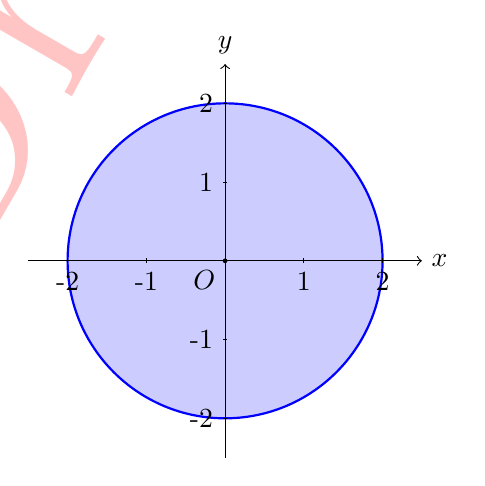
\begin{tikzpicture}[scale=1]
			
			%--- Bán kính ---
			\def\radius{2} % bán kính hình tròn
			
			%--- Vẽ hình tròn ---
			\fill[blue!20] (0,0) circle (\radius);          
			\draw[thick,blue] (0,0) circle (\radius);        
			
			%--- Tâm ---
			\fill (0,0) circle (0.03) node[below left] {$O$};
			
			%--- Trục x ---
			\draw[->] (-2.5,0) -- (2.5,0) node[right] {$x$};
			\foreach \x in {-2,-1,1,2} {
				\draw (\x,0.03) -- (\x,-0.03); % tick mark
				\node[below] at (\x,-0.03) {\x}; % số luôn nằm trên cùng
			}
			
			%--- Trục y ---
			\draw[->] (0,-2.5) -- (0,2.5) node[above] {$y$};
			\foreach \y in {-2,-1,1,2} {
				\draw (0.03,\y) -- (-0.03,\y);
				\node[left] at (-0.03,\y) {\y};
			}
			
		\end{tikzpicture}
	\end{minipage}
	\hfill
	\begin{minipage}[c]{0.35\textwidth}
		\raggedright
		i. $u(r_0,\varphi)=\sin(3\varphi)$;\vskip7pt
		ii. $u(r_0,\varphi)=4+3\cos\varphi$.
	\end{minipage}\\\\
	\textbf{b) }\vskip7pt
	\begin{minipage}[c]{0.15\textwidth}
		\centering
		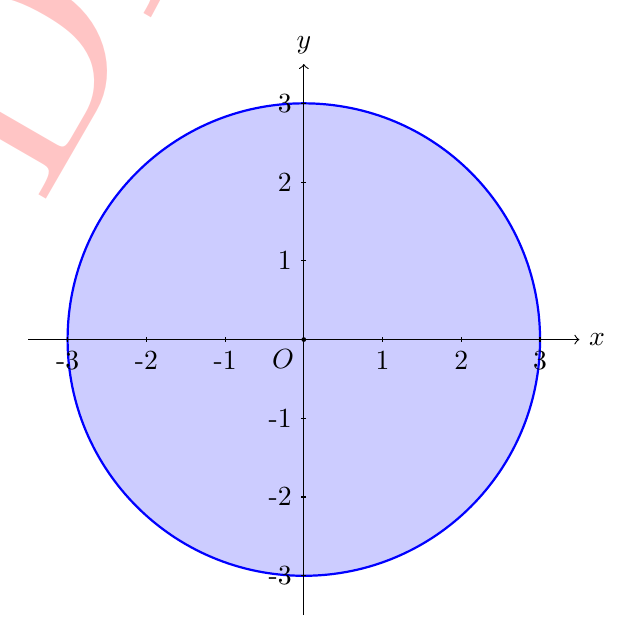
\begin{tikzpicture}[scale=1]
			
			%--- Bán kính ---
			\def\radius{3} % bán kính hình tròn
			
			%--- Vẽ hình tròn ---
			\fill[blue!20] (0,0) circle (\radius);          
			\draw[thick,blue] (0,0) circle (\radius);        
			
			%--- Tâm ---
			\fill (0,0) circle (0.03) node[below left] {$O$};
			
			%--- Trục x ---
			\draw[->] (-3.5,0) -- (3.5,0) node[right] {$x$};
			\foreach \x in {-3,-2,-1,1,2,3} {
				\draw (\x,0.03) -- (\x,-0.03); % tick mark
				\node[below] at (\x,-0.03) {\x}; % số luôn nằm trên cùng
			}
			
			%--- Trục y ---
			\draw[->] (0,-3.5) -- (0,3.5) node[above] {$y$};
			\foreach \y in {-3,-2,-1,1,2,3} {
				\draw (0.03,\y) -- (-0.03,\y);
				\node[left] at (-0.03,\y) {\y};
			}
			
		\end{tikzpicture}
	\end{minipage}
	\hfill
	\begin{minipage}[c]{0.35\textwidth}
		\raggedright
		i. $u(r_0,\varphi)=3+\cos(2\varphi)$;\vskip7pt
		ii. $u(r_0,\varphi)=5\sin^3\varphi$.
	\end{minipage}\\\\
	\textbf{c) }\vskip7pt
	\begin{minipage}[c]{0.15\textwidth}
		\centering
		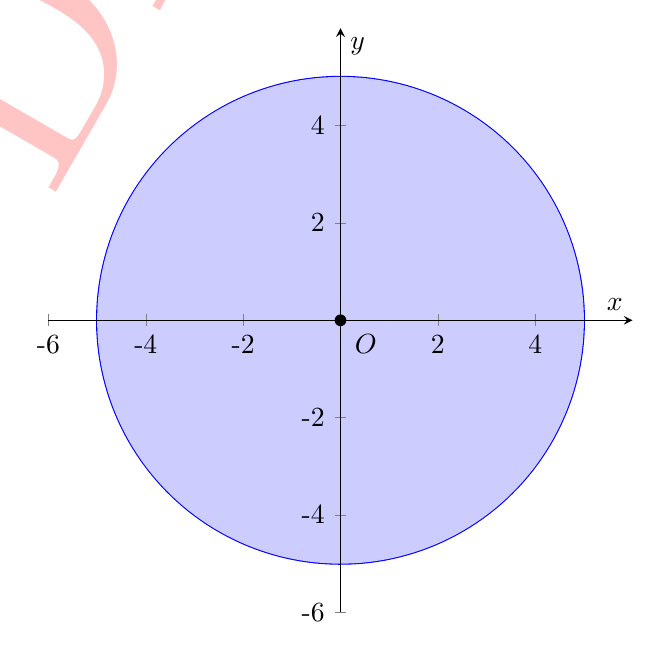
\begin{tikzpicture}[scale=1]
			
			\begin{axis}[
				axis lines=middle,
				xmin=-3, xmax=3,
				ymin=-3, ymax=3,
				xtick={-3,-2,-1,0,1,2},        % vị trí tick thật
				xticklabels={-6,-4,-2,0,2,4},  % nhãn hiển thị khác
				ytick={-3,-2,-1,0,1,2},
				yticklabels={-6,-4,-2,0,2,4},
				grid=none,
				width=9cm, height=9cm,
				xlabel={$x$}, ylabel={$y$},
				enlargelimits=false,
				axis on top,
				]
				
				\addplot[
				domain=0:360,
				samples=200,
				thick, blue,
				] ({2.5*cos(x)},{2.5*sin(x)});
				
				\addplot [
				draw=none,
				fill=blue!20,
				domain=0:360,
				samples=200,
				] ({2.5*cos(x)},{2.5*sin(x)});
				
				\node[circle,fill=black,inner sep=1.5pt,label={-45:$O$}] at (axis cs:0,0) {};
			\end{axis}
			
		\end{tikzpicture}
	\end{minipage}
	\hfill
	\begin{minipage}[c]{0.35\textwidth}
		\raggedright
		i. $u(r_0,\varphi)=6\cos\varphi$;\vskip7pt
		ii. $u(r_0,\varphi)=7+2\sin^2(4\varphi)$.
	\end{minipage}
	\begin{flushleft}
		\textbf{\color{red}\underline{Bài 2:}} Cho hai miền vành khăn sau với bán kính nhỏ là $r_1$ và bán kính lớn là $r_2$. Ứng với mỗi miền, hãy tìm một hàm điều hòa $u(r,\varphi)$ bên trong miền với các phân bố nhiệt tại mép hình vành khăn cho trước.
	\end{flushleft}
	\textbf{a) }\begin{minipage}[c]{0.15\textwidth}
		\centering
		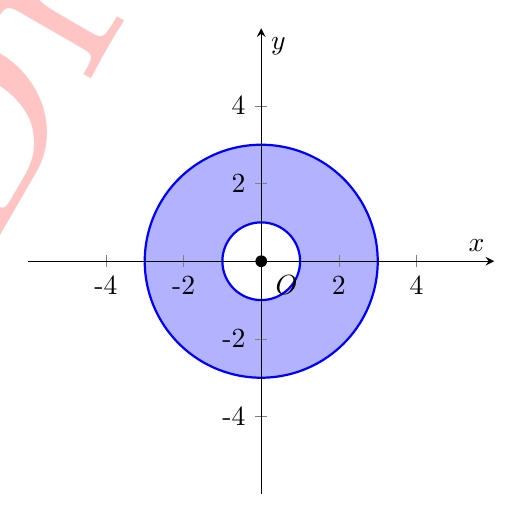
\begin{tikzpicture}[scale=1]
			
			\begin{axis}[
				axis lines=middle,
				xmin=-3, xmax=3,
				ymin=-3, ymax=3,
				xtick={-2,-1,0,1,2},             
				xticklabels={-4,-2,0,2,4},       
				ytick={-2,-1,0,1,2},
				yticklabels={-4,-2,0,2,4},
				width=7.5cm, height=7.5cm,
				xlabel={$x$}, ylabel={$y$},
				enlargelimits=false,
				axis on top,                     
				]
				
				%--- Bán kính ngoài/ trong theo NHÃN ---
				\def\Rout{1.5} % thật = 3/2
				\def\Rin{0.5}  % thật = 1/2
				
				%=== 1. Tô hình tròn ngoài (R2) ===
				\addplot [
				draw=none,
				fill=blue!30,
				domain=0:360,
				samples=200,
				] ({\Rout*cos(x)},{\Rout*sin(x)});
				
				%=== 2. Tô lại hình tròn trong (R1) bằng màu nền để tạo lỗ ===
				\addplot [
				draw=none,
				fill=white,
				domain=0:360,
				samples=200,
				] ({\Rin*cos(x)},{\Rin*sin(x)});
				
				%=== 3. Viền ngoài và viền trong ===
				\addplot [thick,blue,domain=0:360,samples=200] ({\Rout*cos(x)},{\Rout*sin(x)});
				\addplot [thick,blue,domain=0:360,samples=200] ({\Rin*cos(x)},{\Rin*sin(x)});
				
				%--- Đánh dấu gốc O ---
				\node[circle,fill=black,inner sep=1.5pt,label={-45:$O$}] at (axis cs:0,0) {};
				
			\end{axis}
			
		\end{tikzpicture}
	\end{minipage}
	\hfill
	\begin{minipage}[c]{0.45\textwidth}
		\raggedright
		i. $\begin{cases}
			u(r_1,\varphi)=\cos(2\varphi),\\
			u(r_2,\varphi)=5\sin\varphi;
		\end{cases}$\vskip7pt
		ii. $\begin{cases}
			u(r_1,\varphi)=1+3\cos^2(3\varphi),\\
			\noalign{\vskip5pt}
			u(r_2,\varphi)=\dfrac52+4\sin\varphi.
		\end{cases}$
	\end{minipage}\\\\\\
	\textbf{b) }\begin{minipage}[c]{0.15\textwidth}
		\centering
		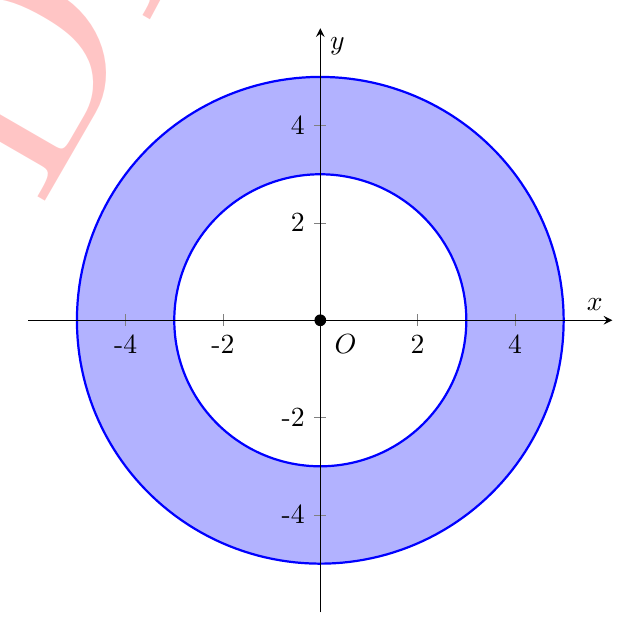
\begin{tikzpicture}[scale=1]
			
			\begin{axis}[
				axis lines=middle,
				xmin=-3, xmax=3,
				ymin=-3, ymax=3,
				xtick={-2,-1,0,1,2},             
				xticklabels={-4,-2,0,2,4},       
				ytick={-2,-1,0,1,2},
				yticklabels={-4,-2,0,2,4},
				width=9cm, height=9cm,
				xlabel={$x$}, ylabel={$y$},
				enlargelimits=false,
				axis on top,                     
				]
				
				%--- Bán kính ngoài/ trong theo NHÃN ---
				\def\Rout{2.5} % thật = 5/2
				\def\Rin{1.5}  % thật = 3/2
				
				%=== 1. Tô hình tròn ngoài (R2) ===
				\addplot [
				draw=none,
				fill=blue!30,
				domain=0:360,
				samples=200,
				] ({\Rout*cos(x)},{\Rout*sin(x)});
				
				%=== 2. Tô lại hình tròn trong (R1) bằng màu nền để tạo lỗ ===
				\addplot [
				draw=none,
				fill=white,
				domain=0:360,
				samples=200,
				] ({\Rin*cos(x)},{\Rin*sin(x)});
				
				%=== 3. Viền ngoài và viền trong ===
				\addplot [thick,blue,domain=0:360,samples=200] ({\Rout*cos(x)},{\Rout*sin(x)});
				\addplot [thick,blue,domain=0:360,samples=200] ({\Rin*cos(x)},{\Rin*sin(x)});
				
				%--- Đánh dấu gốc O ---
				\node[circle,fill=black,inner sep=1.5pt,label={-45:$O$}] at (axis cs:0,0) {};
				
			\end{axis}
			
		\end{tikzpicture}
	\end{minipage}
	\hfill
	\begin{minipage}[c]{0.45\textwidth}
		\raggedright
		i. $\begin{cases}
			u(r_1,\varphi)=2\ln27+1+4\cos(2\varphi),\\
			u(r_2,\varphi)=2\ln125+1+6\sin\varphi\cos(2\varphi);
		\end{cases}$\vskip7pt
		ii. $\begin{cases}
			u(r_1,\varphi)=3\sin(2\varphi),\\
			u(r_2,\varphi)=4\cos^3\varphi.
		\end{cases}$
	\end{minipage}
	\begin{flushleft}
		\textbf{\color{red}\underline{Bài 3:}} Từ các hình chữ nhật cho ở bên dưới (mỗi cạnh tương ứng với một hàm số), hãy thành lập phương trình Laplace với các điều kiện biên, và tìm nghiệm của chúng.\vskip20pt
	\end{flushleft}
	\begin{minipage}[c]{0.15\textwidth}
		\centering
		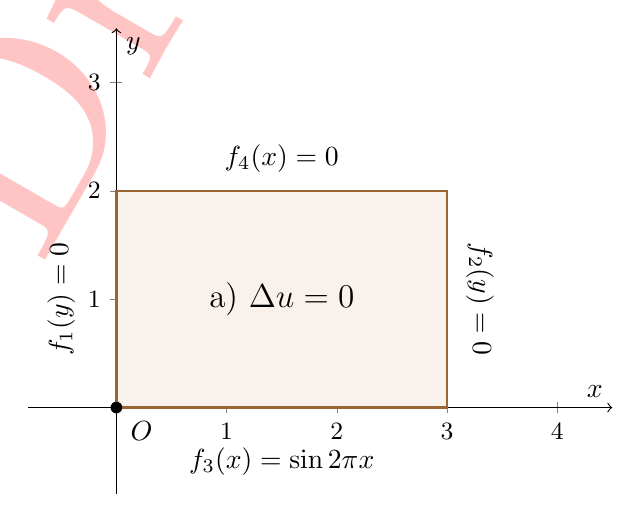
\begin{tikzpicture}[scale=1]
			
			\begin{axis}[
				axis lines=middle,
				xmin=-0.8, xmax=4.5,
				ymin=-0.8, ymax=3.5,
				width=9cm, height=7.5cm,
				xlabel={$x$}, ylabel={$y$},
				xtick={0,1,2,3,4},
				ytick={0,1,2,3},
				axis line style={->},
				tick label style={font=\small},
				enlargelimits=false,         % mũi tên trục
				]
				
				%--- Vẽ hình chữ nhật từ (0,0) đến (3,2) ---
				\addplot[
				draw=brown!80!black,
				fill=brown!10,
				thick
				] coordinates {(0,0) (3,0) (3,2) (0,2) (0,0)};
				
				%--- Viết phương trình biên ---
				\node[rotate=90] at (axis cs:-0.5,1) {$f_1(y)=0$};
				\node[rotate=-90] at (axis cs:3.3,1) {$f_2(y)=0$};
				\node at (axis cs:1.5,2.3) {$f_4(x)=0$};
				\node at (axis cs:1.5,-0.5) {$f_3(x)=\sin 2\pi x$};
				
				%--- Viết phương trình trong miền ---
				\node at (axis cs:1.5,1) {\large a) $\Delta u = 0$};
				
				\node[circle,fill=black,inner sep=1.5pt,label={-45:$O$}] at (axis cs:0,0) {};
				
			\end{axis}
			
		\end{tikzpicture}
	\end{minipage}
	\hfill
	\begin{minipage}[c]{0.45\textwidth}
		\centering
		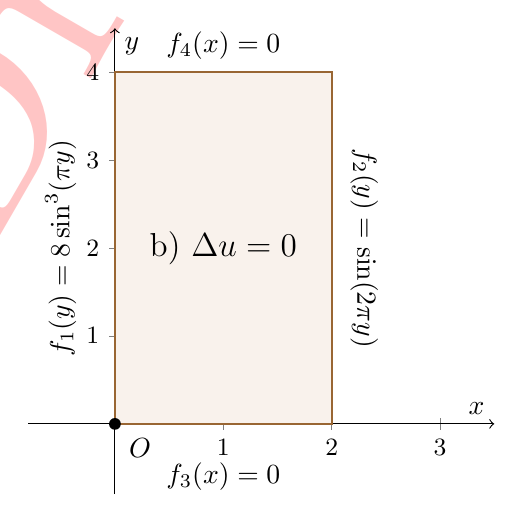
\begin{tikzpicture}[scale=1]
			
			\begin{axis}[
				axis lines=middle,
				xmin=-0.8, xmax=3.5,
				ymin=-0.8, ymax=4.5,
				width=7.5cm, height=7.5cm,
				xlabel={$x$}, ylabel={$y$},
				xtick={0,1,2,3},
				ytick={0,1,2,3,4},
				axis line style={->},
				tick label style={font=\small},
				enlargelimits=false,         % mũi tên trục
				]
				
				%--- Vẽ hình chữ nhật từ (0,0) đến (2,4) ---
				\addplot[
				draw=brown!80!black,
				fill=brown!10,
				thick
				] coordinates {(0,0) (2,0) (2,4) (0,4) (0,0)};
				
				%--- Viết phương trình biên ---
				\node[rotate=90] at (axis cs:-0.5,2) {$f_1(y)=8\sin^3(\pi y)$};
				\node[rotate=-90] at (axis cs:2.3,2) {$f_2(y)=\sin(2\pi y)$};
				\node at (axis cs:1,4.3) {$f_4(x)=0$};
				\node at (axis cs:1,-0.6) {$f_3(x)=0$};
				
				%--- Viết phương trình trong miền ---
				\node at (axis cs:1,2) {\large b) $\Delta u = 0$};
				
				\node[circle,fill=black,inner sep=1.5pt,label={-45:$O$}] at (axis cs:0,0) {};
				
			\end{axis}
			
		\end{tikzpicture}
	\end{minipage}\\\\\\\\
	\begin{minipage}[c]{0.15\textwidth}
		\centering
		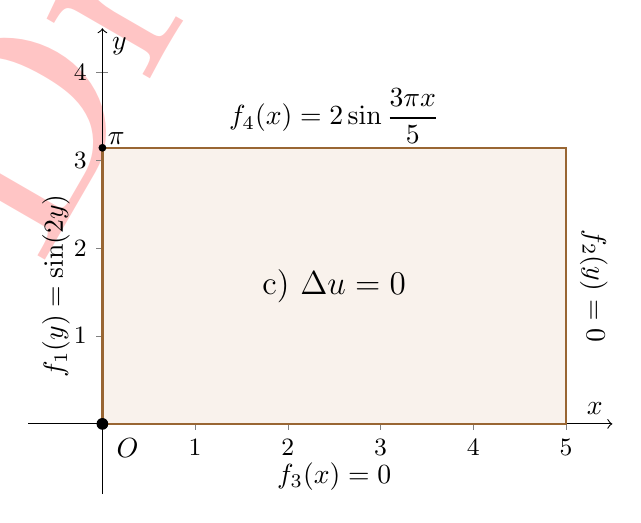
\begin{tikzpicture}[scale=1]
			
			\begin{axis}[
				axis lines=middle,
				xmin=-0.8, xmax=5.5,
				ymin=-0.8, ymax=4.5,
				width=9cm, height=7.5cm,
				xlabel={$x$}, ylabel={$y$},
				xtick={0,1,2,3,4,5},
				ytick={0,1,2,3,4},
				axis line style={->},
				tick label style={font=\small},
				enlargelimits=false,         % mũi tên trục
				]
				
				%--- Vẽ hình chữ nhật từ (0,0) đến (5,pi) ---
				\addplot[
				draw=brown!80!black,
				fill=brown!10,
				thick
				] coordinates {(0,0) (5,0) (5,3.14) (0,3.14) (0,0)};
				
				%--- Viết phương trình biên ---
				\node[rotate=90] at (axis cs:-0.5,1.57) {$f_1(y)=\sin(2y)$};
				\node[rotate=-90] at (axis cs:5.3,1.57) {$f_2(y)=0$};
				\node at (axis cs:2.5,3.5) {$f_4(x)=2\sin\dfrac{3\pi x}{5}$};
				\node at (axis cs:2.5,-0.6) {$f_3(x)=0$};
				\node at (axis cs:0.15,3.25) {$\pi$};
				\node[circle,fill=black,inner sep=1pt] at (axis cs:0,3.14) {};
				
				%--- Viết phương trình trong miền ---
				\node at (axis cs:2.5,1.57) {\large c) $\Delta u = 0$};
				
				\node[circle,fill=black,inner sep=1.5pt,label={-45:$O$}] at (axis cs:0,0) {};
				
			\end{axis}
			
		\end{tikzpicture}
	\end{minipage}
	\hfill
	\begin{minipage}[c]{0.45\textwidth}
		\centering
		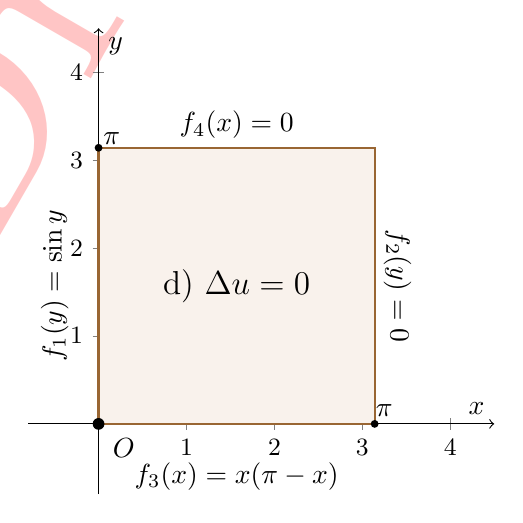
\begin{tikzpicture}[scale=1]
			
			\begin{axis}[
				axis lines=middle,
				xmin=-0.8, xmax=4.5,
				ymin=-0.8, ymax=4.5,
				width=7.5cm, height=7.5cm,
				xlabel={$x$}, ylabel={$y$},
				xtick={0,1,2,3,4},
				ytick={0,1,2,3,4},
				axis line style={->},
				tick label style={font=\small},
				enlargelimits=false,         % mũi tên trục
				]
				
				%--- Vẽ hình chữ nhật từ (0,0) đến (2,4) ---
				\addplot[
				draw=brown!80!black,
				fill=brown!10,
				thick
				] coordinates {(0,0) (3.14,0) (3.14,3.14) (0,3.14) (0,0)};
				
				%--- Viết phương trình biên ---
				\node[rotate=90] at (axis cs:-0.5,1.57) {$f_1(y)=\sin y$};
				\node[rotate=-90] at (axis cs:3.4,1.57) {$f_2(y)=0$};
				\node at (axis cs:1.57,3.4) {$f_4(x)=0$};
				\node at (axis cs:1.57,-0.6) {$f_3(x)=x(\pi -x)$};
				\node at (axis cs:0.15,3.25) {$\pi$};
				\node[circle,fill=black,inner sep=1pt] at (axis cs:0,3.14) {};
				\node at (axis cs:3.25,0.15) {$\pi$};
				\node[circle,fill=black,inner sep=1pt] at (axis cs:3.14,0) {};
				
				%--- Viết phương trình trong miền ---
				\node at (axis cs:1.57,1.57) {\large d) $\Delta u = 0$};
				
				\node[circle,fill=black,inner sep=1.5pt,label={-45:$O$}] at (axis cs:0,0) {};
				
			\end{axis}
			
		\end{tikzpicture}
	\end{minipage}\\\\\\
	\textbf{\color{red}\underline{Bài 4:}} Tìm nghiệm của các bài toán sau với điều kiện biên hỗn hợp. Cho biết giá trị lớn nhất và nhỏ nhất của $u$ trên miền đã cho.
	\begin{flushleft}
		\textbf{a) }$\begin{cases}
			\begin{array}{ll}
				\Delta u=u_{xx}+u_{yy}=0, & 0<x<2,~0<y<4,\\
				\noalign{\vskip5pt}
				u_x(0,y)=u(2,y)=0, & 0\le y\le 4,\\
				\noalign{\vskip4pt}
				u(x,0)=2\cos\dfrac{9\pi x}{4},~u(x,4)=0, & 0\le x\le2.
			\end{array}
		\end{cases}$\vskip7pt
		\textbf{b) }$\begin{cases}
			\begin{array}{ll}
				\Delta u=u_{xx}+u_{yy}=0, & 0<x<0.5\pi,~0<y<2,\\
				u(0,y)=u_x(0.5\pi,y)=0, & 0\le y\le 2,\\
				u(x,0)=0,~u(x,2)=\sin(7x), & 0\le x\le0.5\pi;
			\end{array}
		\end{cases}$\vskip7pt
		\textbf{c) }$\begin{cases}
			\begin{array}{ll}
				\Delta u=u_{xx}+u_{yy}=0, & 0<x<1,~0<y<3,\\
				\noalign{\vskip5pt}
				u(0,y)=0,\,u_x(1,y)=\dfrac{5\pi}6\sin\dfrac{5\pi y}{6}, & 0\le y\le 3,\\
				\noalign{\vskip4pt}
				u(x,0)=u_y(x,3)=0, & 0\le x\le1.
			\end{array}
		\end{cases}$
	\end{flushleft}
	\textbf{\color{red}\underline{Bài 5:}} Tìm nghiệm của các phương trình Poisson sau.
	\begin{flushleft}
		\textbf{a) }$\begin{cases}
			\begin{array}{ll}
				-\Delta u=-u_{xx}-u_{yy}=3x, & 0<x<3,~0<y<4,\\
				u(0,y)=u(3,y)=0, & 0\le y\le4,\\
				u(x,0)=u(x,4)=0, & 0\le x\le3.
			\end{array}
		\end{cases}$\vskip7pt
		\textbf{b) }$\begin{cases}
			\begin{array}{ll}
				-\Delta u=-u_{xx}-u_{yy}=\sin(\pi x)\sin(\pi y), & 0<x<1,~0<y<3,\\
				u(0,y)=u(1,y)=0, & 0\le y\le3,\\
				u(x,0)=u(x,3)=0, & 0\le x\le1;
			\end{array}
		\end{cases}$\vskip7pt
		\textbf{c) }$\begin{cases}
		\begin{array}{ll}
			-\Delta u=-u_{xx}-u_{yy}=\mathrm e^{x+y}, & 0<x<2,~0<y<5,\\
			u(0,y)=u(2,y)=0, & 0\le y\le5,\\
			u(x,0)=u(x,5)=0, & 0\le x\le2.
		\end{array}
		\end{cases}$
	\end{flushleft}
	\newpage
	\section{Phép biến đổi Laplace}
	\subsection{Định nghĩa}
	\quad\,\,\,Cho $f(t)$ là hàm số thực theo biến $t$ và xác định với mọi $t\ge0$. \textbf{\color{red}Biến đổi Laplace} của $f$ được định nghĩa là một hàm $F(s)$ với biến phức $s$, ký hiệu là $\mathcal L(f)$, và được cho bởi $$\boxed{\color{blue}F(s)=\mathcal L(f):=\displaystyle\int_{0^-}^\infty\mathrm e^{-st}f(t)\text{d}t.}$$
	
	Hàm $f(t)$ có thể là hàm mang giá trị phức của biến thực $t$, tức là $f(t)=f_1(t)+\mathrm if_2(t)$ với $f_1$ và $f_2$ là các hàm thực.\\
	
	Biến đổi Laplace là một \textbf{\color{red}biến đổi tích phân}. Điều này nghĩa là phép biến đổi này sẽ biến đổi một hàm từ không gian này sang không gian khác bởi một phép tích phân có \textbf{\color{red}nhân} (kernel), nghĩa là hàm gồm các biến trong hai không gian. Một cách cụ thể, biến đổi Laplace $$F(s)=\int_{0}^\infty K(s,t)f(t)\text{d}t$$
	có nhân là hàm $K(s,t)=\mathrm e^{-st}$.
	\subsection{Phép biến đổi Laplace ngược}
	\quad\,\,\,Hàm $f(t)$ cho trong định nghĩa ở mục 12.1 được gọi là \textbf{\color{red}biến đổi Laplace ngược} của $F(s)$, và được ký hiệu là $\mathcal L^{-1}(F)=:f(t)$. Với định nghĩa này, ta có $$\boxed{\color{blue}\mathcal L^{-1}\big(\mathcal L(f)\big)=f~~\text{và}~~\mathcal L\big(\mathcal L^{-1}(F)\big)=F.}$$
	\subsection{Sự tồn tại phép biến đổi Laplace}
	\quad\,\,\,Nếu $f(t)$ được xác định và là hàm liên tục từng khúc trên mỗi khoảng hữu hạn trong nửa trục số thực $t\ge0$, và thỏa điều kiện tăng trưởng mũ $$|f(t)|\le M\mathrm e^{Kt},~\forall t\ge0,$$
	với hằng số dương $M$ và $K$ nào đó, thì biến đổi Laplace của $f$ tồn tại trong nửa mặt phẳng phức với $\mathfrak R(s)>K$.\\
	
	Nếu $s\in\mathbb R$ thì biến đổi Laplace tồn tại với mọi $s>K$.
	\subsection{Tính duy nhất và tuyến tính}
	\quad~\,$\bullet~$Nếu phép biến đổi Laplace của một hàm tồn tại, thì hàm biến đổi này là \textit{duy nhất}.
	\vskip7pt
	$\bullet~$Nếu hai hàm \textit{liên tục} có cùng phép biến đổi Laplace, thì hai hàm đó bằng nhau.
	\vskip7pt
	$\bullet~$Nếu $f(t)$ và $g(t)$ là hai hàm có biến đổi Laplace và $a,b$ là các hằng số, thì ta có tính tuyến tính
	$$\boxed{\color{blue}\mathcal L[af(t)+bg(t)]=a\mathcal L[f(t)]+b\mathcal L[g(t)],}$$
	và phép biến đổi Laplace ngược cũng có tính tuyến tính như trên.\\
	
	\textbf{Ví dụ 1:} \textit{Tìm biến đổi Laplace của hàm $f(t)=1$ với mọi $t$ không âm.}\\
	
	\textit{Giải.} Vì $f(t)=1$ là hàm liên tục với mọi $t\ge0$ nên biến đổi Laplace của $f$ tồn tại. Khi đó $$\mathcal L(1)=\lim_{T\to\infty}\int_0^T\mathrm e^{-st}1\mathrm dt=\lim_{T\to\infty}\dfrac{-\mathrm e^{-st}}{s}\Bigg|_{t=0}^{t=T}=\lim_{T\to\infty}\left(\frac{1-\mathrm e^{-sT}}{s}\right)=\frac1s-0=\frac1s,$$
	nếu $s>0$. Vậy $\mathcal L(1)=\dfrac1s$ với $s>0$.\\
	
	\textbf{Ví dụ 2:} \textit{Tìm biến đổi Laplace của hàm $f(t)=\mathrm e^{3t}$ với mọi $t$ không âm.}\\
	
	\textit{Giải.} Vì $f(t)=\mathrm e^{3t}$ là hàm liên tục với mọi $t\ge0$ nên biến đổi Laplace của $f$ tồn tại. Khi đó $$\mathcal L(f)=\lim_{T\to\infty}\int_0^T\mathrm e^{(3-s)t}\mathrm dt=\lim_{T\to\infty}\dfrac{\mathrm e^{-(s-3)t}}{3-s}\Bigg|_{t=0}^{t=T}=\lim_{T\to\infty}\left(\frac{\mathrm e^{-(s-3)T}-1}{3-s}\right)=\frac1{s-3},$$
	nếu $s-3>0$. Vậy ta có $\mathcal L(\mathrm e^{3t})=\dfrac{1}{s-3}$ nếu $s>3$.\\
	
	\textbf{Ví dụ 3:} \textit{Tìm biến đổi Laplace của hai hàm hyperbolic} $$f(t)=\cosh(at)=\frac{\mathrm e^{at}+\mathrm e^{-at}}{2}~~\textit{và}~~g(t)=\sinh(at)=\frac{\mathrm e^{at}-\mathrm e^{-at}}{2}.$$
	
	\textit{Giải.} Vì $f(t)$ là hàm liên tục với mọi $t\ge0$ nên biến đổi Laplace của $f$ tồn tại. Khi đó, do tính tuyến tính của phép biến đổi Laplace, ta có $$\mathcal L[\cosh(at)]=\frac12\mathcal L(\mathrm e^{at})+\frac12\mathcal L(\mathrm e^{-at})=\frac{1}{2(s-a)}+\frac{1}{2(s+a)}=\frac{s}{s^2-a^2},$$
	nếu $s>|a|$. Tương tự với $g(t)$, ta cũng có $$\mathcal L[\sinh(at)]=\frac12\mathcal L(\mathrm e^{at})-\frac12\mathcal L(\mathrm e^{-at})=\frac{1}{2(s-a)}-\frac{1}{2(s+a)}=\frac{a}{s^2-a^2},$$
	nếu $s>|a|.$\\
	
	\textbf{Ví dụ 4:} \textit{Chứng minh rằng với $n=0,1,2,\ldots$ thì} $$\mathcal L(t^n)=\frac{n!}{s^{n+1}}.$$
	
	\textit{Giải.} Vì $f(t):=t^n$ là hàm liên tục với mọi $t\ge0$ nên tồn tại biến đổi Laplace của $f$. Bằng quy nạp, trước hết ta kiểm tra trường hợp $n=0$, tức là $$\mathcal L(t^0)=\mathcal L(1)=\frac1s.$$
	
	Điều này đúng theo Ví dụ 1 trên. Giả sử đẳng thức đúng với bất kỳ $n>0$, và ta cần chứng minh $$\mathcal L(t^{n+1})=\frac{(n+1)!}{s^{n+2}}.$$
	
	Thật vậy, sử dụng tích phân từng phần, ta có \begin{align*}
		\mathcal L(t^{n+1})&=\int_0^\infty\mathrm e^{-st}t^{n+1}\mathrm dt\\
		\noalign{\vskip3pt}
		&=-\frac1s\mathrm e^{-st}t^{n+1}\Bigg|_{t=0}^{t\to\infty}+\frac{n+1}{s}\int_0^\infty\mathrm e^{-st}t^n\mathrm dt\\
		\noalign{\vskip5pt}
		&=\frac{n+1}{s}\mathcal L(t^n)=\frac{n+1}{s}\frac{n!}{s^{n+1}}=\frac{(n+1)!}{s^{n+2}}.
	\end{align*}
	
	Vậy ta có điều phải chứng minh.\\
	
	$\bullet~$\textbf{Định lý $\mathbf s$--shifting}: Giả sử hàm $f(t)$ có biến đổi Laplace là $F(s)$ với $s>K$. Khi đó ta có phép biến đổi của $\mathrm e^{at}f(t)$ là $$\boxed{\color{blue}\mathcal L\left[\mathrm e^{at}f(t)\right]=F(s-a)~~\text{hay}~~\mathrm e^{at}f(t)=\mathcal L^{-1}[F(s-a)],~~s-a>K.}$$
	
	\textbf{Ví dụ 5:} \textit{Tìm biến đổi Laplace của hàm $f(t)=\mathrm e^{2t}\cosh(at)$ và hàm $g(t)=\mathrm e^{3t}\sinh(at)$.}\\
	
	\textit{Giải.} Ta đặt $F(s)=\mathcal L[\cosh(at)]=\dfrac{s}{s^2-a^2}$ và $G(s)=\mathcal L[\sinh(at)]=\dfrac{a}{s^2-a^2}$. Khi đó $$\mathcal L(f)=F(s-2)=\frac{s-2}{(s-2)^2-a^2};\hspace{0.5cm}\mathcal L(g)=G(s-3)=\dfrac{a}{(s-3)^2-a^2}.$$
	
	\textbf{Ví dụ 6:} \textit{Tìm biến đổi Laplace ngược của} $$\mathcal L(f)=\frac{2s+26}{s^2-4s-32}.$$
	
	\textit{Giải.} Ta có $$\frac{2s+26}{s^2-4s-32}=\frac{2s-4+30}{(s-2)^2-36}=2\frac{s-2}{(s-2)^2-6^2}+5\frac{6}{(s-2)^2-6^2}.$$
	
	Khi đó do tính tuyến tính của phép biến đổi Laplace ngược và nhờ vào Định lý $s$--shifting, ta có \begin{align*}
		f(t)&=\mathcal L^{-1}\left(\frac{2s+26}{s^2-4s-32}\right)\\
		\noalign{\vskip5pt}
		&=2\mathcal L^{-1}\left[\frac{s-2}{(s-2)^2-6^2}\right]+5\mathcal L^{-1}\left[\frac{6}{(s-2)^2-6^2}\right]\\
		\noalign{\vskip5pt}
		&=2\mathrm e^{2t}\cosh(6t)+5\mathrm e^{2t}\sinh(6t)\\
		&=\mathrm e^{2t}[2\cosh(6t)+5\sinh(6t)].
	\end{align*}
	\subsection{Biến đổi Laplace của đạo hàm}
	\quad\,\,\,$\bullet~$\textbf{Định lý:} Cho $f,f',\ldots,f^{(n-1)}$ là các hàm liên tục với mọi $t\ge0$ và thỏa điều kiện tăng ở mục 12.3. Giả sử đạo hàm $f^{(n)}$ liên tục từng khúc trên mỗi khoảng hữu hạn với $t\ge0$. Khi đó ta có biến đổi Laplace của đạo hàm bậc cao được định nghĩa là $$\boxed{\color{blue}\mathcal L\big[f^{(n)}\big]=s^n\mathcal L(f)-s^{n-1}f(0)-s^{n-2}f'(0)-\cdots-f^{(n-1)}(0).}$$
	
	\textbf{Ví dụ 1:} \textit{Tìm biến đổi Laplace của $f(t)=t\sinh(\omega t)$.}\\
	
	\textit{Giải.} Ta tính \begin{align*}
		&f(0)=0,\\
		&f'(t)=\sinh(\omega t)+\omega t\cosh(\omega t),~~f'(0)=0,\\
		&f''(t)=2\omega\cosh(\omega t)+\omega^2t\sinh(\omega t).
	\end{align*}
	
	Sử dụng định nghĩa của phép biến đổi Laplace, ta có $$\mathcal L(f'')=\int_0^\infty\mathrm e^{-st}\big[2\omega\cosh(\omega t)+\omega^2t\sinh(\omega t)\big]\mathrm dt=2\omega\frac{s}{s^2-\omega^2}+\omega^2\mathcal L(f).$$
	
	Mặt khác, công thức biến đổi Laplace của đạo hàm cho ta $$\mathcal L(f'')=s^2\mathcal L(f)-sf(0)-f'(0)=s^2\mathcal L(f).$$
	
	Kết hợp lại, ta được phương trình $$2\omega\frac{s}{s^2-\omega^2}+\omega^2\mathcal L(f)=s^2\mathcal L(f)\iff2\omega\frac{s}{s^2-\omega^2}=(s^2-\omega^2)\mathcal L(f)\iff\mathcal L(f)=\frac{2\omega s}{(s^2-\omega^2)^2}.$$
	
	Vậy $\mathcal L[t\sinh(\omega t)]=\dfrac{2\omega s}{(s^2-\omega^2)^2}$.\\
	
	\textbf{Ví dụ 2 (Ứng dụng giải ODE):} \textit{Giải bài toán Cauchy sau bằng phép biến đổi Laplace} $$\begin{cases}
		y''(t)-4y(t)=8t,\\
		y(0)=5,\\
		y'(0)=0.
	\end{cases}$$
	
	\textit{Giải.} Đặt $Y(s)=\mathcal L[y(t)]$ là biến đổi Laplace của $f(t)$. Áp dụng phép biến đổi Laplace vào hai vế của phương trình, ta có \begin{align*}
		&\mathcal L[y''(t)-4y(t)]=\mathcal L(8t)\\
		\Leftrightarrow~&s^2Y(s)-sy(0)-y'(0)-4Y(s)=\frac{8}{s^2}\\
		\Leftrightarrow~&(s^2-4)Y(s)-5s-0=\frac{8}{s^2}\\
		\Leftrightarrow~&(s^2-4)Y(s)=\frac{8}{s^2}+5s\\
		\Leftrightarrow~&Y(s)=\frac{8}{s^2(s^2-4)}+\frac{5s}{s^2-4}.
	\end{align*}
	
	Ta có $$\frac{8}{s^2(s^2-4)}+\frac{5s}{s^2-4}=\frac{2}{s^2-4}-\frac{2}{s^2}+\frac{5s}{s^2-4},$$
	nên biến đổi Laplace ngược cho ta \begin{align*}
		y(t)&=\mathcal L^{-1}\left(\frac{2}{s^2-4}\right)-2\mathcal L^{-1}\left(\frac{1}{s^2}\right)+5\mathcal L^{-1}\left(\frac{s}{s^2-4}\right)=\sinh(2t)-2t+5\cosh(2t)\\
		\noalign{\vskip5pt}
		&=\frac{\mathrm e^{2t}-\mathrm e^{-2t}}{2}-2t+\frac{5\mathrm e^{2t}+5\mathrm e^{-2t}}{2}=3\mathrm e^{2t}+2\mathrm e^{-2t}-2t.
	\end{align*}
	\subsection{Hàm bước Heaviside - Ứng dụng giải phương trình đạo hàm riêng}
	\quad\,\,\,$\bullet~$\textbf{Định nghĩa hàm bước Heaviside (hàm bước đơn vị):} là hàm $H(t-a)$ được định nghĩa như sau $$H(t-a)=\begin{cases}
		0,~~t<a,\\
		1,~~t>a,
	\end{cases}$$
	với $x=a$ là điểm mà tại đó hàm này gián đoạn (có thể nhận giá trị 1 hoặc không xác định). Dưới đây là đồ thị của hàm $H(t-a)$.
	\begin{center}
		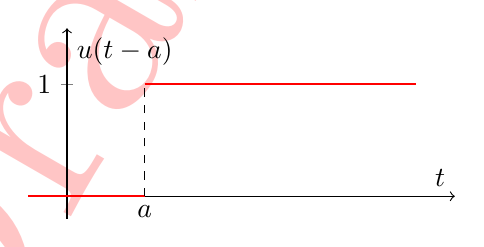
\begin{tikzpicture}
			\begin{axis}[
				axis lines=middle,
				xmin=-0.2, xmax=2,
				ymin=-0.2, ymax=1.5,
				width=7cm, height=4cm,
				xtick=\empty,
				ytick={0,1},
				yticklabels={0,1},
				xlabel={$t$}, ylabel={$u(t-a)$},
				enlargelimits=false,
				axis line style={->},
				]
				
				%--- Đặt vị trí a (số thực giữa 0 và 1) ---
				\def\a{0.4}
				
				%--- Đoạn từ 0 đến a: 0 ---
				\addplot[
				draw=red!100!black,
				thick
				] coordinates {(-0.2,0) (\a,0)};
				
				%--- Đoạn từ a đến 1.8: 1 ---
				\addplot[
				draw=red!100!black,
				thick
				] coordinates {(\a,1) (1.8,1)};
				
				%--- Đường nét đứt tại a ---
				\addplot[black,dashed] coordinates {(\a,0) (\a,1)};
				
				%--- Nhãn a ---
				\node[below] at (axis cs:\a,0) {$a$};
				
			\end{axis}
		\end{tikzpicture}
	\end{center}
	
	Biến đổi Laplace của hàm bước Heaviside với $a>0$ là $$\mathcal L[H(t-a)]=\int_a^\infty\mathrm e^{-st}\mathrm dt=\frac{-\mathrm e^{-st}}{s}\Bigg|_{t=a}^{t\to\infty}=\frac{\mathrm e^{-sa}}{s},~~s>0.$$
	
	Hàm bước đơn vị có ứng dụng trong kỹ thuật để biểu diễn những hàm có trạng thái ‘đóng’ hay ‘mở’. Một cách cụ thể, cho $f(t)=0$ với $t<0$. Khi đó $f(t-a)H(t-a)$ với $a>0$ chính là hàm $f(t)$ mà được \textbf{\color{red}dịch chuyển sang phải} $a$ đơn vị.\\
	
	$\bullet~$\textbf{Định lý $\mathbf t$--shifting:} Nếu $f(t)$ có biến đổi Laplace là $F(s)$, thì \textit{hàm dịch chuyển} $$\widetilde f(t)=f(t-a)H(t-a)=\begin{cases}
		\begin{array}{ll}
			0, & t<a, \\
			f(t-a), & t>a,
		\end{array}
	\end{cases}$$
	có biến đổi Laplace là $$\boxed{\color{blue}\mathcal L[f(t-a)H(t-a)]=\mathrm e^{-as}F(s).}$$
	
	Tương tự, ta cũng có công thức $$\boxed{\color{blue}\mathcal L[f(t)H(t-a)]=\mathrm e^{-as}\mathcal L[f(t+a)].}$$
	
	\textbf{Ví dụ 1:} \textit{Tìm biến đổi Laplace ngược của} $$F(s)=\frac{\mathrm e^{-s}}{s^2-4\pi^2}+\frac{s\mathrm e^{-3s}}{s^2-16}+\frac{\mathrm 4e^{-4s}}{(s-3)^3}.$$
	
	\textit{Giải.} Ta lưu ý rằng \begin{align*}
		&\mathcal L^{-1}\left(\frac{1}{s^2-4\pi^2}\right)=\frac{1}{2\pi}\sinh(2\pi t),\\
		\noalign{\vskip5pt}
		&\mathcal L^{-1}\left(\frac{s}{s^2-16}\right)=\cosh(4t),\\
		\noalign{\vskip5pt}
		&\mathcal L^{-1}\left[\frac{2}{(s-3)^3}\right]=t^2\mathrm e^{3t}.
	\end{align*}
	
	Ở đây, biến đổi Laplace thứ ba thu được bằng Định lý $s$--shifting cho $\mathcal L(t^2)=\dfrac{2}{s^3}=F(s)$, nghĩa là $$F(s-a)=\frac{2}{(s-a)^3}=\mathcal L[\mathrm e^{at}f(t)]~\text{với}~a=3.$$
	
	Do đó Định lý $t$--shifting cho ta \begin{align*}
		f(t)&=\mathcal L^{-1}\left(\mathrm e^{-s}\frac{1}{s^2-4\pi^2}\right)+\mathcal L^{-1}\left(\mathrm e^{-3s}\frac{s}{s^2-16}\right)+2\mathcal L^{-1}\left[\mathrm e^{-4s}\frac{2}{(s-3)^3}\right]\\
		\noalign{\vskip5pt}
		&=\frac{1}{2\pi}\sinh[2\pi(t-1)]H(t-1)+\cosh[4(t-3)]H(t-3)+2(t-4)^2\mathrm e^{3(t-4)}H(t-4)\\
		\noalign{\vskip5pt}
		&=\frac{1}{2\pi}\sinh[2\pi(t-1)]H(t-1)+\cosh(4t-12)H(t-3)+2(t-4)^2\mathrm e^{3t-12}H(t-4).
	\end{align*}
	
	\textbf{Ví dụ 2 (Ứng dụng giải PDE):} \textit{Tìm nghiệm của phương trình đạo hàm riêng} $$\begin{cases}
		u_t+u_x+3u=0,\\
		u(0,t)=\sinh(5t),\\
		u(x,0)=0.
	\end{cases}$$
	
	\textit{Giải.} Gọi $U(x,s)=\mathcal L[u(x,t)](s,t)=\displaystyle\int_0^\infty\mathrm e^{-st}u(x,t)\mathrm dt$ là biến đổi Laplace của $u(x,t)$ theo biến $t$.\\
	
	Lấy biến đổi Laplace hai vế của phương trình theo biến $t$, ta có \begin{align*}
		&\mathcal L[u_t(x,t)+u_x(x,t)+3u(x,t)]=0\\
		\Leftrightarrow~&sU(x,s)-u(x,0)+U_x(x,s)+3U(x,s)=0\\
		\Leftrightarrow~&U_x(x,s)+(s+3)U(x,s)=0,
	\end{align*}
	và ta cũng có $U(0,s)=\mathcal L[\sinh(5t)]=\dfrac{5}{s^2-25}$.\\
	
	Phương trình vi phân theo $U(x,s)$ vừa thu được có nghiệm $$U(x,s)=\frac{5\mathrm e^{-(s+3)x}}{s^2-25}=\mathrm e^{-3x}\frac{5\mathrm e^{-xs}}{s^2-25},$$
	nên theo Định lý $t$--shifting, nghiệm của PDE ban đầu là $$u(x,t)=\mathrm e^{-3x}\sinh[5(t-x)]H(t-x)=\frac{\mathrm e^{5t-8x}-\mathrm e^{2x-5t}}{2}H(t-x).$$
	\subsection{Bảng biến đổi Laplace của một số hàm thông dụng}
	\begin{multicols}{2}
		\begin{center}
			\renewcommand{\arraystretch}{2.0}
			\begin{tabular}{|c|c|}
				\hline
				\textbf{\color{red}Hàm số} & \textbf{\color{red}Biến đổi Laplace} \\ \hline 
				1 & $\dfrac1s$ \\[4pt] \hline 
				$\mathrm e^{at}$ & $\dfrac{1}{s-a}$ \\[4pt] \hline 
				$t^n$ & $\dfrac{n!}{s^{n+1}}$ \\[4pt] \hline
				$\sin(at)$ & $\dfrac{a}{s^2+a^2}$ \\[4pt] \hline 
				$\cos(at)$ & $\dfrac{s}{s^2+a^2}$ \\[4pt] \hline
				$\sinh(at)$ & $\dfrac{a}{s^2-a^2}$ \\[4pt] \hline 
				$\cosh(at)$ & $\dfrac{s}{s^2-a^2}$ \\[4pt] \hline
				$\mathrm e^{at}t^n$ & $\dfrac{n!}{(s-a)^{n+1}}$ \\[4pt] \hline
				$\mathrm e^{at}\sin(bt)$ & $\dfrac{b}{(s-a)^2+b^2}$ \\[4pt] \hline 
				$\mathrm e^{at}\cos(bt)$ & $\dfrac{s-a}{(s-a)^2+b^2}$ \\[4pt] \hline
			\end{tabular}
		\end{center}
		\columnbreak
		\begin{center}
			\renewcommand{\arraystretch}{2.0}
			\begin{tabular}{|c|c|}
				\hline
				\textbf{\color{red}Hàm số} & \textbf{\color{red}Biến đổi Laplace} \\ \hline 
				$\mathrm e^{at}\sinh(bt)$ & $\dfrac{b}{(s-a)^2-b^2}$ \\[4pt] \hline 
				$\mathrm e^{at}\cosh(bt)$ & $\dfrac{s-a}{(s-a)^2-b^2}$ \\[4pt] \hline
				$t\sin(at)$ & $\dfrac{2as}{(s^2+a^2)^2}$ \\[4pt] \hline 
				$t\cos(at)$ & $\dfrac{s^2-a^2}{(s^2+a^2)^2}$ \\[4pt] \hline
				$f'(t)$ & $sF(s)-f(0)$ \\[4pt] \hline 
				$f''(t)$ & $s^2F(s)-sf(0)-f'(0)$ \\[4pt] \hline
				$\displaystyle\int_0^tf(u)\text{d}u$ & $\dfrac1sF(s)$ \\[4pt] \hline 
				$t^nf(t)$ & $(-1)^n\dfrac{\text{d}^n}{\text{d}s^n}\big(F(s)\big)$ \\[4pt] \hline
				$\dfrac1tf(t)$ & $\displaystyle\int_s^\infty F(s)\text{d}s$ \\[4pt] \hline 
				$\delta(t)$ & 1 \\[4pt] \hline
			\end{tabular}
		\end{center}
	\end{multicols}
	\subsection{Bài tập tự luyện}
	\color{red}\textbf{\underline{Bài 1:}} \color{black} Tìm biến đổi Laplace của các hàm số sau với $t\ge0$. \begin{multicols}{2}
		\begin{flushleft}
			\textbf{a) }$f(t)=\begin{cases}
				\begin{array}{ll}
					2, & 0\le t<3, \\
					t^2-6t+9, & t\ge3;
				\end{array}
			\end{cases}$\\\vspace{3mm}
			\textbf{b) }$f(t)=t\mathrm e^{-3t}\cos2t;$
		\end{flushleft}
		\columnbreak
		\begin{flushleft}
			\textbf{c) }$f(t)=(t-2)^2H(t-2);$\\\vspace{3mm}
			\textbf{d) }$f(t)=\sinh6t\cosh t+\cosh6t\sinh t+2\cosh^24t-1$;\\\vspace{3mm}
			\textbf{e) }$f(t)=4\mathrm e^{4t}t^3+3\mathrm e^{4t}t^2.$
		\end{flushleft}
	\end{multicols}
	\begin{flushleft}
		\color{red}\textbf{\underline{Bài 2:}} \color{black} Tìm biến đổi Laplace ngược của các hàm số sau.
	\end{flushleft}
	\begin{multicols}{2}
		\begin{flushleft}
			\textbf{a) }$F(s)=\dfrac{s-2}{s^2-12s+52};$\\\vspace{3mm}
			\textbf{c) }$F(s)=\dfrac{s+1}{(s-2)^2(s+4)};$
		\end{flushleft}
		\columnbreak
		\begin{flushleft}
			\textbf{b) }$F(s)=\dfrac{3\mathrm e^{-2t}+1}{s^2-10s-9}.$\\\vspace{3mm}
			\textbf{d) }$F(s)=\dfrac{s^2+8s-3}{(s^2+2s+1)(s^2+1)}.$
		\end{flushleft}
	\end{multicols}
	\begin{flushleft}
		\color{red}\textbf{\underline{Bài 3:}} \color{black} Bằng phương pháp biến đổi Laplace, hãy tìm nghiệm $y(t)$ của các ODE sau đây.
	\end{flushleft}
	\begin{multicols}{2}
		\begin{flushleft}
			\textbf{a) }$\begin{cases}
				y''-2y'-y=0,\\
				y(0)=-1,\,y'(0)=1;
			\end{cases}$
		\end{flushleft}
		\begin{flushleft}
			\textbf{c) }$\begin{cases}
				y''+4y=\delta(t-1),\\
				y(0)=3,\,y'(0)=0;
			\end{cases}$
		\end{flushleft}
		\columnbreak
		\begin{flushleft}
			\textbf{b) }$\begin{cases}
				y''-y=t\mathrm e^{2t},\\
				y(0)=0,\,y'(0)=1;
			\end{cases}$
		\end{flushleft}
		\begin{flushleft}
		\textbf{d) }$\begin{cases}
			y''+6y'+18y=3H(\pi-t),\\
			y(0)=y'(0)=0.
		\end{cases}$
		\end{flushleft}
	\end{multicols}
	\color{red}\textbf{\underline{Bài 4:}} \color{black}Bằng phương pháp biến đổi Laplace, hãy tìm nghiệm $u(x,t)$ của các PDE sau đây.
	\begin{multicols}{2}
		\begin{flushleft}
			\textbf{a) }$\begin{cases}
				\begin{array}{ll}
					u_t+u_x=2x, & x>0,~t>0, \\
					u(0,t)=0, & t\ge0,\\
					u(x,0)=0, & x\ge0;
				\end{array}
			\end{cases}$
		\end{flushleft}
		\begin{flushleft}
			\textbf{c) }$\begin{cases}
				\begin{array}{ll}
					u_t+2u_x=x+t, & x>0,~t>0, \\
					u(0,t)=0, & t\ge0,\\
					u(x,0)=0, & x\ge0;
				\end{array}
			\end{cases}$
		\end{flushleft}
		\begin{flushleft}
			\textbf{e) }$\begin{cases}
				\begin{array}{ll}
					u_t=4u_{xx}, & 0<x<2,~t>0, \\
					u(0,t)=u(2,t)=0, & t\ge0,\\
					u(x,0)=2\sin(2\pi x), & x\ge0;
				\end{array}
			\end{cases}$
		\end{flushleft}
		\columnbreak
		\begin{flushleft}
			\textbf{b) }$\begin{cases}
				\begin{array}{ll}
					u_t+u_x+u=0, & x>0,~t>0, \\
					u(0,t)=0, & t\ge0,\\
					u(x,0)=\cos x, & x\ge0;
				\end{array}
			\end{cases}$
		\end{flushleft}
		\begin{flushleft}
			\textbf{d) }$\begin{cases}
				\begin{array}{ll}
					u_t=u_{xx}, & x>0,~t>0, \\
					u_x(0,t)=\mathrm e^{-t}, & t\ge0,\\
					u(x,0)=0, & x\ge0;
				\end{array}
			\end{cases}$
		\end{flushleft}
		\begin{flushleft}
			\textbf{f) }$\begin{cases}
				\begin{array}{ll}
					u_t=16u_{xx}, & 0<x<\pi,~t>0, \\
					u(0,t)=u(\pi,t)=0, & t\ge0,\\
					u(x,0)=4\sin(5x), & x\ge0.
				\end{array}
			\end{cases}$
		\end{flushleft}
	\end{multicols}
\newpage
\begin{thebibliography}{1}
\bibitem[1]{1} Nguyễn Thành Long, \textit{\href{https://drive.google.com/file/d/1RPRrqId9-08bfTKazocns1gklrmpyDrM/view?usp=drive_link}{Phương trình toán lý}}, Bộ môn Giải tích, Khoa Toán - Tin học, Trường Đại học Khoa học tự nhiên, ĐHQG-HCM, 2017.

\bibitem[2]{2} Peter V.O' Neil, \textit{\href{https://libgen.is/book/index.php?md5=D24358102866676081EED6FF319C84E6}{Beginning Partial Differential Equations}}, The University of Alabama and Birmingham, John Wiley \& Sons, Inc., 2008.

\bibitem[3]{3} Lawrence C. Evans, \textit{\href{https://libgen.is/book/index.php?md5=6D9DF85A10396346D4CD5261DEE06AC4}{Partial Differential Equations}}, Graduate Studies in Mathematics, vol. 19, American Mathematical Society, 1998.

\bibitem[4]{4} Russell Herman, \textit{\href{https://math.libretexts.org/Bookshelves/Differential_Equations/Introduction_to_Partial_Differential_Equations_(Herman)}{Introduction to Partial Differential Equations}}, University of North Carolina Wilmington, LibreTexts Mathematics, 2024.

\bibitem[5]{5} Slide bài giảng Phương trình toán lý của TS. Lê Đức Hưng, Bộ môn Giải tích, Khoa Toán - Tin học, Trường Đại học Khoa học tự nhiên, ĐHQG-HCM.
\end{thebibliography}
\end{document}